\documentclass[11pt,a4paper]{article}
\usepackage[T1]{fontenc}
\usepackage{lmodern}
\usepackage[margin=27mm]{geometry}
\usepackage{amsmath,amssymb,amsthm,mathtools}
\renewcommand{\qedsymbol}{\textnormal{\small Q.E.D.}}
\usepackage{graphicx,booktabs,longtable,array,tabularx,multirow}
\newcolumntype{P}[1]{>{\raggedright\arraybackslash}p{#1}}
\renewcommand{\tabularxcolumn}[1]{P{#1}}
\usepackage[table]{xcolor}
\usepackage{microtype}
\usepackage{enumitem}
\usepackage{caption,subcaption}
\usepackage[section]{placeins}
\usepackage[numbers,sort&compress]{natbib}
\usepackage{xurl}
\usepackage[colorlinks=true,linkcolor=blue!45!black,citecolor=blue!45!black,urlcolor=blue!45!black]{hyperref}
\hypersetup{pdftitle={Kobon Triangle Constructions: Uniform Lower Bounds, Structural Defect Bounds, and Formal Verification},pdfauthor={Alejandro Zarzuelo Urdiales},pdfsubject={Exact constructions, geometric successor rules, structural upper bounds, and Lean verification}}
\usepackage[nameinlink,noabbrev]{cleveref}
\usepackage{listings}
\usepackage{fancyhdr}
\setlength{\headheight}{14pt}
\pagestyle{fancy}
\fancyhf{}
\fancyhead[L]{\small Kobon triangle constructions and formal verification}
\fancyhead[R]{\small A. Zarzuelo Urdiales}
\fancyfoot[C]{\thepage}
\renewcommand{\headrulewidth}{0.25pt}
\setlength{\emergencystretch}{2em}
\makeatletter
\renewcommand{\l@subsection}{\@dottedtocline{2}{1.5em}{3.4em}}
\makeatother
\setlength{\parskip}{3pt}
\setlist{itemsep=2pt,topsep=4pt}
\captionsetup{font=small,labelfont=bf,margin=5mm}
\setcounter{topnumber}{3}
\setcounter{bottomnumber}{2}
\setcounter{totalnumber}{5}
\renewcommand{\topfraction}{0.92}
\renewcommand{\bottomfraction}{0.85}
\renewcommand{\textfraction}{0.07}
\renewcommand{\floatpagefraction}{0.7}
\graphicspath{{figures/}}
\newtheorem{theorem}{Theorem}[section]
\newtheorem{proposition}[theorem]{Proposition}
\newtheorem{lemma}[theorem]{Lemma}
\newtheorem{corollary}[theorem]{Corollary}
\theoremstyle{definition}
\newtheorem{definition}[theorem]{Definition}
\newtheorem{conjecture}[theorem]{Conjecture}
\theoremstyle{remark}
\newtheorem{remark}[theorem]{Remark}
\newcommand{\K}{K}
\newcommand{\Ks}{K_{\mathrm{s}}}
\newcommand{\G}{G}
\newcommand{\B}{B}
\newcommand{\N}{\mathbb{N}}
\newcommand{\R}{\mathbb{R}}
\newcommand{\Z}{\mathbb{Z}}
\newcommand{\U}{U}
\newcommand{\Lbound}{L}
\newcommand{\floor}[1]{\left\lfloor#1\right\rfloor}
\newcommand{\ceil}[1]{\left\lceil#1\right\rceil}
\newcommand{\lean}[1]{{\small\nolinkurl{#1}}}
\newcommand{\repo}{\url{https://github.com/alejandrozu/kobon-proof}}
\newcommand{\proofref}[3]{\href{https://github.com/alejandrozu/kobon-proof/blob/f44f23ee062a255f5cad7d39188fd55c0feb83a8/#1\#L#2}{#3}}
\newcommand{\sourcefile}[2]{\href{https://github.com/alejandrozu/kobon-proof/blob/f44f23ee062a255f5cad7d39188fd55c0feb83a8/#1}{#2}}
\newcommand{\status}[1]{\textsf{\small[#1]}}
\DeclareMathOperator{\sgn}{sgn}
\DeclareMathOperator{\conv}{conv}
\DeclareMathOperator{\intt}{int}
\lstset{basicstyle=\ttfamily\footnotesize,breaklines=true,columns=fullflexible,keepspaces=true,frame=single,framerule=0.3pt,rulecolor=\color{black!25},xleftmargin=4pt,xrightmargin=4pt}
\title{Kobon Triangle Constructions:\\Uniform Lower Bounds, Structural Defect Bounds,\\and Formal Verification}
\author{Alejandro Zarzuelo Urdiales}
\date{Comprehensive research edition, 7 October 2026}
\begin{document}
\maketitle
\begin{abstract}
The Kobon triangle problem asks for the largest number of bounded triangular cells determined by real affine lines. We consolidate a construction and verification program begun in March 2026, including the research of 5--6 October. An all-order simple construction gives $G(n)=\floor{n(n-3)/3}+1+(n\bmod2)$ for $n\ge4$. Compatible geometric seeds now instantiate the proved Bartholdi--Blanc--Loisel recursion at orders based on $32$, $36$, $48$, and $60$, alongside the earlier eleven-derived family. For $q=60\cdot2^t$, actual simple arrangements give $1200\cdot4^t-10$ triangles at $q+1$ and $1200\cdot4^t+30\cdot2^t-11$ at $q+2$, respectively nine and ten below the simple upper floors. Poola supplied the finite $61:1190$ count; the uniform compatible refit and its 29-pair visibility certificate are the developments here. An executable portfolio retains the earlier all-order envelope. The quantitative deficit-dependent successor stated in the previous edition now has a complete actual-geometric Lean proof and indefinite iteration for both parities. We also extract nonsimple core fans, matching and components from actual arrangements, proving degree-free mixed-multiplicity defect bounds and sharper all-triple bounds with positive local contributions. Exact translation germs yield birth/loss identities and interval counterexamples to a specific desingularization loss formula. The inherited numerical families, standard axioms, finite native checks, external classifications and bounded unsuccessful searches are distinguished throughout. The unrestricted Kobon problem and the arbitrary full half-order successor remain unresolved; no worldwide numerical-priority claim is made.
\end{abstract}
\vspace{0.4em}
\noindent\textbf{Keywords.} Line arrangements; triangular cells; Kobon problem; constructive lower bounds; projective transformations; exact computation; Lean formalization.
\clearpage
\tableofcontents
\clearpage
\section{Introduction and scope of the results}\label{sec:introduction}

An arrangement of $n$ straight lines divides the real plane into bounded and unbounded cells. The Kobon problem asks how many of the bounded cells can be triangles. The difficulty is not creating many triples of intersecting lines: there are $\binom n3$ candidate triples. The difficulty is ensuring that their triangles are not cut by any of the remaining lines and that their interiors do not overlap. The distinction between an attractive picture and a valid arrangement is therefore central to both construction and verification.

Let $\K(n)$ denote the classical maximum, allowing multiple intersections and parallel lines, and let $\Ks(n)$ denote the maximum over simple arrangements: no parallel pair and no three concurrent lines. All lower-bound witnesses constructed by the universal theorem below are simple, so they establish lower bounds for both quantities. Some of the strongest retained finite certificates are nonsimple. We never use an upper bound restricted to $\Ks$ as an upper bound for $\K$ without an additional argument.

This paper consolidates the author's March 2026 extension proposal and the subsequent program of exact construction, comparison with the literature, and formal proof. The purpose is both mathematical and documentary: to state the strongest completed results, to make their proofs and provenance inspectable, and to preserve the failed approaches that determine the next research questions. The original general extension claim is reported as an unresolved claim rather than silently promoted to a theorem.

\subsection{The main completed all-order theorem}

Define $\B(n)=\ceil{n(n-3)/3}$ for $n\ge3$, and set $\B(n)=0$ for $n<3$. The familiar F\"uredi--Pal\'asti construction supplies this affine baseline; the underlying construction and its historical priority belong to the earlier literature~\cite{furedipalasti1984,erickson1999}. The first completed all-order theorem is the following refinement; the recursive envelope below now strengthens its retained finite enhancement.

\begin{theorem}[Universal affine refinement]\label{thm:main}
For every $n\in\N$, there is a simple arrangement of $n$ real straight lines with at least $\G(n)$ bounded triangular cells, where
\begin{equation}\label{eq:G}
\G(n)=\begin{cases}
0,&0\le n<3,\\
1,&n=3,\\
\floor{n(n-3)/3}+1+(n\bmod2),&n\ge4.
\end{cases}
\end{equation}
Consequently $\K(n)\ge\Ks(n)\ge\G(n)$.
\end{theorem}

The proof, developed in Section~\ref{sec:universal}, combines a shifted trigonometric arrangement with one- and two-cap changes of affine chart. The Lean declaration \lean{Kobon.Universal.baseline_sound} proves the geometric existence statement for arbitrary $n$. It has no assumed extension theorem and no dependence on finite experimental verification. Its dependencies are the standard logical axioms used by Lean and Mathlib.

For $n\ge4$, the gains over $\B(n)$ are $1,1,0,2,0,1$ in residue classes $0,1,2,3,4,5$ modulo six. Thus the refinement is strict at every odd order at least five and every positive multiple of six. Both formulas have leading behavior $n^2/3-n+O(1)$: this is a constant-term refinement, not an improved quadratic or linear asymptotic coefficient. The original F\"uredi--Pal\'asti projective count table already contains related constants. The present source audit does not establish first numerical priority for the affine formula.

\begin{figure}[tbp]
\centering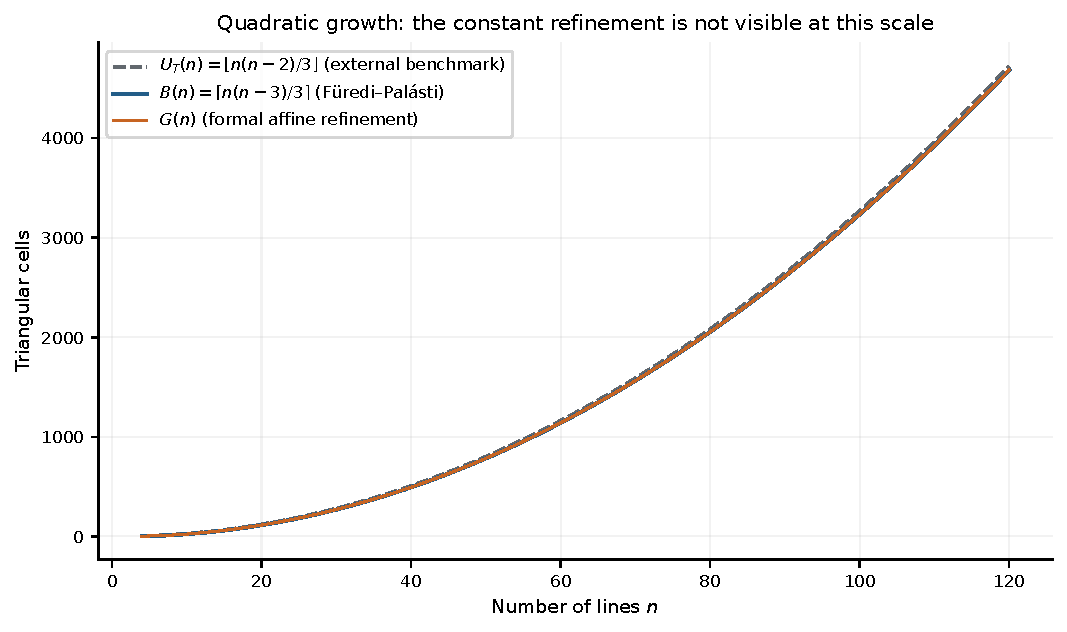
\includegraphics[width=0.94\linewidth]{bounds-growth.pdf}
\caption{Growth of the classical general baseline, the proved affine refinement, and the classical polynomial upper benchmark. The close overlap on a quadratic scale is mathematically meaningful: the new uniform gain is bounded. Residue and deficit plots below resolve the smaller differences. This figure is computed from the formulas, not copied from earlier publications.}\label{fig:growth}
\end{figure}

\subsection{Finite enhancements and other completed components}

The universal construction is supplemented by exact coordinates. Let $C(n)$ be the largest triangle count among the finite certificates in the release at order $n$, with $C(n)=0$ when no such certificate is saved. Then
\begin{equation}\label{eq:envelope}
\Lbound(n)=\max\{\G(n),C(n)\},\qquad \K(n)\ge\Lbound(n)
\end{equation}
is proved for all natural orders. This elementary maximum operation retains published constructions and the author's earlier values without altering their attribution. It is not a claim that $\Lbound$ is the largest lower bound obtainable from all published constructions by every possible interpolation or extension.

The finite catalog contains 138 distinct coordinate certificates, including 104 simple witnesses. A separate generated table has 64 orders at which a saved finite certificate strictly improves the older baseline $\B$; some of these improvements are already supplied by $\G$. The catalog includes weaker checkpoints and independent reproductions. Its size is not a count of original discoveries.

The 2 October release added a recursively closed geometric family. Put
$q_t=10\cdot2^t$ and $A_t=(q_t^2-4)/3$. For every $t\ge0$, simple
arrangements realize at least $A_t$ triangles at $q_t+1$ lines and
$A_t+q_t/2$ at $q_t+2$ lines. Every next seed retains the sorted grid,
saturation, positive central apex and visible-boundary data. Taking
the maximum of these candidates and $\Lbound$ gives the earlier total
bound $H$ of Theorem~\ref{fam:all-n-envelope}. It strictly improves
the previous repository envelope at every family pair from 321/322
onward, without claiming a new literature record for the inherited
numerical family.

The research of 5--6 October completes the compatible 33- and 49-line
seed proofs, adds the known 37-line orbit, and realizes a further
60-dyadic orbit from Poola's 61-line point input. Its strongest even
branch uses 29 visible pairs. The resulting portfolio $J$ retains $H$
pointwise (Theorem~\ref{fam:portfolio}). These are actual straight-line
witnesses at every finite depth; their historical attributions and
simple-model gaps appear in Table~\ref{fam:orbit-table}.

The earlier manuscript's quantitative boundary-defect successor now has
an end-to-end Lean proof, including terminal-ray extraction and averaging,
and it iterates through both parities. The original full half-order
recurrence remains unproved. On the upper side, actual cyclic fans,
side matching, graph components and geometric escape are now extracted
from the arrangement. The strongest all-triple global estimate is
\[
 2\delta+B_{15}\ge2U+3(E_3+P_{21})+N_{12}+M_{22},
\]
with the local counts defined in Section~\ref{upper:degree-free}.
Mixed-multiplicity and component estimates retain explicit corrections;
they do not yield an unrestricted numerical bound depending only on $n$.
The translation analysis of Section~\ref{sec:surgery} proves exact
birth/loss accounting and counterexamples to a specified loss formula.
Table~\ref{tab:claims} separates these claims from the still open problem.

\begin{table}[tbp]
\centering\small
\begin{tabularx}{\linewidth}{@{}P{0.28\linewidth}XP{0.21\linewidth}@{}}
\toprule
Result & Mathematical content & Release status\\
\midrule
Universal $\G$ & Simple real-line witnesses at every order & General Lean proof\\
Envelope $\Lbound$ & Maximum with all saved finite witnesses & Lean; finite native checks\\
28:238, 30:275, 34:357 & Earlier attributed finite inequalities & Exact Lean certificates\\
Exterior extension & New line and gain from a visible-pair list & General Lean proof\\
Full successor recurrence & $\K(n+1)\ge\K(n)+\floor{n/2}$ & Unproved\\
49-seed numerical target & Lower function obtained by summing the proposed recurrence & Independently proved\\
One-step BBL doubling & $(q+1,T)\mapsto(2q+1,T+q^2)$ for compatible seeds & General Lean proof\\
Infinite hybrid iteration & Odd and full-gain even geometric families & Complete Lean; native seed\\
33/37/49 orbits & Known numerical families, compatible real seeds and simple optimality & Complete Lean; native seeds\\
61 orbit & Uniform $1190/29$ seed; constant simple gaps 9 and 10 & Complete Lean; native seed\\
Quantitative successor & Deficit-dependent actual rule, both parities, indefinite iteration & General Lean proof\\
Local fan structure & Incidence, antipodal and run-length restrictions & General Lean proofs\\
Simple upper windows & Actual odd/even upper bounds and family existence & Complete Lean\\
Actual clean-line charging & Charge existence and finite fiber bounds & General Lean proof\\
Global multiplicity consequences & Actual fans, matching, mixed and triple defect estimates & General Lean proofs; class scope\\
Local surgery & Exact translation germs, retention, births and losses & General Lean proofs\\
Loss-rule counterexamples & Four- and six-line real parameter intervals & General Lean proofs\\
Tangent-grid obstruction & Explicit ten-sign algebraic impossibility & General Lean proof\\
\bottomrule
\end{tabularx}
\caption{Claim status in the 7 October edition. ``General Lean proof'' does not imply that every proposed application has been formalized. Published construction inputs retain their original authorship.}\label{tab:claims}
\end{table}

\subsection{History, attribution, and the structure of the paper}

The March archive records a proposed extension from odd to even orders, associated finite bounds, and an incomplete Lean file. That file contains eight proof placeholders, including its central extension step. Later exact certificates establish the finite inequalities independently, while the current all-order proof uses a different construction. Accordingly, a corrected account must separate the survival of numerical conclusions from the validity of the original proof strategy.

The September work broadened the program to both parities, exterior visibility, boundary-defect estimates, compatible doubling seeds, exact rational realization, and multiplicity-sensitive upper arguments. Several plausible routes failed: direct repetition of exterior gains lost the necessary boundary resources; small perturbations of nonsimple records sometimes reduced the triangle count; and large local searches failed to improve their chosen seeds. These negative findings retain their finite scope. The 2 October work closed the recursive and clean-line interfaces and added grid obstructions. The 5--6 October work closes the quantitative successor and actual nonsimple fan extraction, strengthens structural component bounds, and isolates exact surgery losses. The unrestricted full-gain successor and unrestricted numerical upper problem remain open.

Section~\ref{sec:geometry} states the geometric definitions and the certificate-to-cell bridge. Section~\ref{sec:universal} proves the uniform refinement; Section~\ref{sec:finite} records finite cases and provenance. The following sections develop extension and family results, local upper-bound ingredients, and computational searches. The final sections describe the formal trust boundary and future obligations. The appendices contain the complete finite tables and a map from mathematical claims to proof sources. The code and evidence are available at \repo~\cite{zarzueloRepository}.

\section{Literature, provenance, and the scope of comparison}
\label{lit:review}

\subsection{Four distinctions that affect every comparison}

The literature studies several related extremal functions. Their numerical tables cannot be combined without retaining their hypotheses. Throughout this paper, $\K(n)$ concerns straight lines in the real affine plane and permits multiple intersections and parallel pairs, whereas $\Ks(n)$ restricts to pairwise nonparallel lines with no three concurrent. Only bounded triangular cells are counted. A pseudoline arrangement is a topological relaxation; a lower bound obtained there becomes a straight-line lower bound only after realizability has been established. Finally, projective triangular faces need not remain bounded after an affine chart is chosen.

\begin{table}[htbp]
\centering\small
\begin{tabularx}{\textwidth}{@{}lXX@{}}
\toprule
Distinction & What transfers immediately & What requires another argument\\
\midrule
Simple / unrestricted & A simple example is an unrestricted example. & A simple upper bound need not bound a configuration with concurrent lines.\\
Straight / pseudoline & Every straight arrangement is a pseudoline arrangement. & A pseudoline construction requires a straight realization.\\
Affine / projective & Projective transformations preserve incidence and projective faces. & Boundedness depends on the line chosen as infinity.\\
Finite / infinite & A certified configuration proves its individual lower bound. & Iteration requires the next configuration to satisfy every input invariant.\\
\bottomrule
\end{tabularx}
\caption{Logical distinctions used throughout the source audit.}
\label{lit:scope-table}
\end{table}

There are also two different projective-to-affine operations. Choosing a new line at infinity outside an $n$-line arrangement keeps $n$ lines, but may lose triangular faces to infinity. Making one of the arrangement's own lines the line at infinity and removing it produces an $(n-1)$-line affine arrangement. The latter operation underlies several optimal subsequences; the former is central to the uniform construction formalized here.

\subsection{From the puzzle to arrangement theory}

Fujimura's puzzle reached English readers through \emph{The Tokyo Puzzles}, edited by Gardner and translated by Adachi~\citep{fujimura1978}; Gardner also discussed it in his collected mathematical recreations~\citep{gardner1983}. The broader theory of line and pseudoline arrangements is developed in Gr\"unbaum's monograph~\citep{grunbaum1972}. The papers of Strommer and Purdy document an established extremal-triangle literature preceding the construction used in this paper~\citep{strommer1977,purdy1979,purdy1980}. We cite those early papers as historical context rather than silently identifying all their projective or non-simple questions with the affine function $\K$.

The familiar comparison polynomial is
\begin{equation}
 U_{\mathrm T}(n)=\left\lfloor\frac{n(n-2)}3\right\rfloor.
 \label{lit:tamura}
\end{equation}
The attribution to Saburo Tamura is transmitted in the Cl\'ement--Bader draft~\citep{clementbader2007}; an original publication by Tamura was not located in this audit. We therefore do not manufacture an independent bibliographic item for that attribution. Cl\'ement and Bader report the stronger classical envelope $U_{\mathrm T}(n)-1$ for $n\equiv0,2\pmod6$. Section~\ref{upper:scope} explains both the scope of this reported result and a local proof-reading issue. A source-reported upper bound and an upper bound proved in our Lean development are different kinds of evidence.

\subsection{The F\"uredi--Pal\'asti all-order construction}

F\"uredi and Pal\'asti gave highly triangular straight-line arrangements using trigonometric coordinates~\citep{furedipalasti1984}. Their projective Table~1 has a residue-dependent constant term. The familiar affine consequence is commonly written
\begin{equation}
 \B(n)=\left\lceil\frac{n(n-3)}3\right\rceil\qquad(n\ge3).
 \label{lit:baseline}
\end{equation}
Erickson states this formula explicitly in Section~7.2 while using arrangements in a computational-geometric lower-bound argument~\citep{erickson1999}. Felsner and Kriegel place the construction in the study of Euclidean triangular cells~\citep{felsnerkriegel1999}. A later discussion by Dam\'asdi, Mart\'inez-Sandoval, Nagy and Nagy quotes the slightly weaker floor version while studying triangle areas~\citep{damasdi2020}. Thus a general lower bound valid at every order existed well before the present work.

Our completed formula is
\begin{equation}
 \G(n)=\left\lfloor\frac{n(n-3)}3\right\rfloor+1+(n\bmod2),
 \qquad n\ge4.
 \label{lit:our-formula}
\end{equation}
The constructions in later sections prove this for actual simple affine lines. Table~\ref{lit:residue-comparison} separates its arithmetic improvement over~\eqref{lit:baseline} from the projective count in the original paper. Here $P_{\mathrm{FP}}(n)$ denotes the latter construction's projective count, not the projective maximum.

\begin{table}[htbp]
\centering\small
\begin{tabular}{@{}cclc@{}}
\toprule
$n\bmod6$ & $\G-\B$ & $P_{\mathrm{FP}}(n)$, $n\ge5$ & $P_{\mathrm{FP}}-\G$\\
\midrule
0 & 1 & $n(n-3)/3$ & $-1$\\
1 & 1 & $(n^2-3n+5)/3$ & $0$\\
2 & 0 & $(n^2-3n+8)/3$ & $2$\\
3 & 2 & $(n^2-3n+9)/3$ & $1$\\
4 & 0 & $(n^2-3n+8)/3$ & $2$\\
5 & 1 & $(n^2-3n+5)/3$ & $0$\\
\bottomrule
\end{tabular}
\caption{Exact comparison with the quoted affine baseline and with the original projective construction's face counts. A projective surplus does not itself supply additional bounded affine triangles.}
\label{lit:residue-comparison}
\end{table}

The numerical gain is bounded by two. In particular, the quadratic coefficient $1/3$ and linear coefficient $-1$ remain unchanged. What the completed proof adds is a phase refinement, a controlled choice of affine chart for odd orders, and an end-to-end geometric formalization. The audited sources do not provide an explicit statement of~\eqref{lit:our-formula} with this affine proof. That observation is not an exhaustive numerical-priority theorem: old projective constructions contain related counts, and an unnoticed affine-chart argument could have been available earlier. The defensible claim is the proved improvement over the explicitly quoted formula~\eqref{lit:baseline}, together with the formal construction; a claim of first numerical discovery is withheld.

\subsection{Optimal subsequences and the straightening problem}

Harborth and Roudneff developed constructions and extremal results for pseudolines~\citep{harborth1985,roudneff1996}. Their scope matters because topological realizability does not imply straight realizability. Forge and Ram\'irez Alfons\'in constructed a projective straight-line family at orders $2\cdot2^t+2$\citep{forge1998}. Removing a distinguished line at infinity gives optimal affine orders $2\cdot2^t+1$; in particular, this is the relevant older source for the $33$-line order.

Bartholdi, Blanc and Loisel's preprint appeared in 2007 and its proceedings publication in 2008~\citep{bbl2008}. Their compatible doubling step takes $q+1$ lines to $2q+1$ and adds $q^2$ triangles. It requires a prescribed tangent grid and a fully used distinguished line. Their straight-line optimal series include $14\cdot2^t+1$ and $6\cdot2^t+1$; their $18\cdot2^t+1$ series was then a pseudoline result. The general numerical recurrence is therefore prior work, not a new theorem of this project. Our contribution is the verified real-coordinate specialization, a closed recursive seed invariant and its boundary-visibility refinement. The actual odd and adjacent-even induction is complete in this release; it does not transfer authorship of the published doubling gain.

Parpalak and Utkin supplied a compatible straight $19$-line seed and established the straight-line series $n=18\cdot2^t+1$\citep{parpalakutkin2026}. Its triangle count is $108\cdot4^t-1$. Substitution into our formula gives the exact comparison
\begin{equation}
 \bigl(108\cdot4^t-1\bigr)-\G(18\cdot2^t+1)=6\cdot2^t-2.
 \label{lit:pu-gap}
\end{equation}
Thus their series is stronger at these orders: the comparisons begin $107>103$ at $19$, $431>421$ at $37$, and $1727>1705$ at $73$. Their separate even-series draft is also relevant prior construction evidence~\citep{parpalakutkinEven2026}. Its numerical families are not replaced by a weaker universal formula.

It would consequently be misleading to call $\G$ the strongest numerical lower bound for every $n$, or an unqualified state of the art among all possible all-order formulas. Taking a maximum with known special constructions already improves it. Padding a configuration by lines sufficiently far away preserves its bounded triangles and extends each special construction to later orders. The retained function in the repository likewise takes a maximum with its finite certificate catalogue. The purpose of $\G$ is a compact uniform guarantee with a complete formal proof, not the suppression of stronger special cases.

\subsection{Upper-bound refinements retain their simplicity assumptions}

The even-order bound
\[
 \left\lfloor\frac{n(n-7/3)}3\right\rfloor
\]
in Bartholdi--Blanc--Loisel applies to \emph{simple affine pseudoline} arrangements. Blanc subsequently proved the sharper common even-order polynomial
\begin{equation}
 \Ks(n)\le\left\lfloor\frac{n(n-5/2)}3\right\rfloor,
 \qquad n\text{ even},
 \label{lit:blanc-even}
\end{equation}
also in the simple pseudoline setting~\citep{blanc2011}. The latter work was posted in 2008 and published in 2011. Its parity argument is the starting point for our clean-line accounting outside a multiple-point core.

The distinction is concrete. Formula~\eqref{lit:blanc-even} equals $53$ at $n=14$, whereas a nonsimple configuration with $54$ triangles exists. Applying a simple upper theorem to that configuration would be invalid. Our upper-bound work therefore counts shared sides and multiple incidences explicitly rather than treating a small perturbation to general position as automatically harmless.

\subsection{Recent computational constructions and versioned claims}

Savchuk's 2025 work combines arrangement tables, SAT search, and heuristic straightening~\citep{savchuk2025}. It reports optimal $23$- and $27$-line configurations and an exclusion of a perfect $33$-triangle arrangement at order $11$. Its Appendix~A.4 records the earlier Honma-based $11$-line construction. For our purposes, an arrangement table, a floating-point fit, an exact straight-line certificate, and an exhaustive upper-bound exclusion are four different outputs. The present work independently verifies the coordinate lower bounds it imports; it does not thereby replay the external SAT exclusions.

Maiorana released fifteen exact $14$-line, $54$-triangle configurations~\citep{maiorana2026}. We preserve their attribution and the source's CC BY 4.0 license. The current Parpalak--Utkin gallery supplies further exact constructions, including nonsimple even-order examples~\citep{parpalakutkinGallery2026}. The $8$-line construction has earlier provenance; citing its current host does not transfer its invention to the host authors. Each retained dataset is tied to a source revision, checked independently, and distinguished from any stronger optimality language used in its original repository.

Versioning also matters for exclusions. The fourth version of Liang, Liu and Zhang's preprint concerns symmetry restrictions for simple $28$-line configurations~\citep{liangliuZhang2026}. It is not treated here as a proof of an unrestricted exact value, and its displayed numerical comparison is not substituted for Blanc's simple upper theorem. The ProofAtlas research page similarly reports restricted upper results while keeping the unrestricted problem open~\citep{proofatlas2026}. We record these as current research sources, not as independently reproduced proofs.

\subsection{The 2026 enumeration and its use as external input}

Parpalak and Utkin's July 2026 preprint gives a reduced-word enumeration
and classification of triangle-maximal pseudoline arrangements, with
Euclidean and projective equivalence kept distinct
\cite{parpalakutkinEnumeration2026}. Its larger first-hit examples are
pseudoline constructions; straight realizability is a separate problem.
The present tangent-grid obstruction uses their supplied 21-line
classification as an external completeness input. Our exact replay
checks the algebraic contradiction certificates and all supplied
affine-class/support cases, not their full enumeration algorithm inside
Lean. Keeping the infinity support and every Euclidean class is
essential: a smaller list of projective representatives did not suffice
for the affine exclusion.

The compatible 49-line branch also requires careful comparison. Its
completed odd family at $n=48\cdot2^t+1$ is the tail of BBL's older
$n=6\cdot2^s+1$ series, with $s=t+3$. The counts cannot be presented as
new lower-bound records. The uniform explicit slopes, whole-interval
sign certificate, boundary data and completed formal seed interface are
the contributions here. The completed 33-line branch likewise verifies
the inherited Forge--Ram\'irez Alfons\'in orbit. The new 37-line seed
verifies the $q=36$ tail of the known Parpalak--Utkin/Blanc numerical
orbit. Formal coverage of these families is not numerical priority.

\subsection{OpenMath inputs and the 5--6 October developments}

The source audit pins Poola's and Srirangam's OpenMath submissions and
the competition judging archive by immutable repository revisions
\cite{poola2026,srirangam2026,openmathJudging2026}. Judging summaries
may precede later compilation receipts; they are evidence of the
competition record, not mathematical authority. Poola's 61-line point
count of 1190 is retained with that attribution. The compatible
reciprocal-slope refit, whole true-tangent interval, and 29-visible-pair
certificate support the 60-dyadic orbit in Section~\ref{fam:seed61}.
The inspected primary sources did not locate this particular straight
orbit, but that bounded comparison does not prove worldwide priority.

Srirangam's local shared-apex, wrong-ray, cap-block and clean-line
arguments informed the upper investigation. Unfinished global transfer
or Hall-capacity arguments from a source packet are not imported as
theorems. Section~\ref{upper:actual-global} instead proves actual fan
and matching extraction and quantifies its component and multiplicity
consequences. Cl\'ement--Bader's earlier perfect-implies-simple claim
keeps its attribution even where its auxiliary shared-side accounting
cannot supply our proof.

Section~\ref{surgery:four} gives a four-line real-parameter counterexample
to the half-plane yield formula in Liu's versioned 2026 desingularization
preprint~\cite{liuDesingularization2026}. Its scope is that formula,
rather than unrelated results or the entire numerical Kobon problem.
The replacement is a global exact germ loss set, with retention requiring
a separate geometric argument.

\subsection{The March result, later verification, and attribution}

The author's March manuscript proposed an even-order extension and recorded the values $238$, $275$, and $357$ at orders $28$, $30$, and $34$\citep{zarzuelo2026}. These values are now supported in this project by exact simple-line certificates. The associated original Lean file, however, contained placeholders, including the general extension lemma. The later successful formalizations do not retroactively turn that unfinished universal argument into a proof.

OEIS A006066 indexes numerical data, references, and named contributions~\citep{oeisA006066}. It is not a complete priority database. In particular, the 2007 Bartholdi--Blanc--Loisel table already contains a bold, hence straight-realizable, $30{:}275$ entry. The $34{:}357$ value follows from the older perfect $33$-line family and its exterior extension. At $28$ lines, Savchuk describes the analogous extension of the $27$-line solution. These overlaps require a distinction between an independently supplied construction, a new exact or formal certificate, and the first known numerical lower bound. We retain the author's recorded contribution without claiming first numerical priority solely from the OEIS attribution.

The recurrence reproduced by HandWiki~\citep{handwiki2026} is likewise a record of the proposed claim rather than a substitute for its proof. The unrestricted statement
\[
 \K(n+1)\ge\K(n)+\left\lfloor n/2\right\rfloor
\]
has not been established by the work reported here. What has been established includes a geometric exterior extension under explicit visibility hypotheses, finite successful successor steps, and a separate unconditional all-order construction. Their logical roles remain distinct.

\subsection{What formal verification contributes}

The proof infrastructure uses Lean~4~\citep{lean4} and mathlib~\citep{mathlib}. For the universal result, it connects analytic line equations, determinant signs, triangular cells, affine-chart control, and finite counting, rather than checking the final arithmetic formula in isolation. For finite results, it turns attributed coordinates into explicit certificates. The upper development now proves actual segment incidence, clean-line charging, classical simple bounds, cyclic-fan and matching extraction, and global structural component inequalities. The remaining numerical upper problem lies in residual local profiles and ordinary-end trade-offs, rather than an assumed extraction bridge.

The accompanying repository~\citep{zarzueloRepository} records source revisions, negative searches, axiom reports, and the boundary between proved statements and proposed research. This separation is part of the result: a complete formal proof of a modest uniform improvement is stronger evidence than an ambitious recurrence with an unproved geometric step. It does not by itself confer numerical priority or solve the unrestricted Kobon problem.

\section{Real-line geometry and exact certificates}\label{sec:geometry}

\subsection{The two extremal problems}
\begin{definition}
An affine line is a set $\{(x,y)\in\R^2:ax+by=c\}$ with $(a,b)\ne(0,0)$. An arrangement is a finite set of distinct lines. A triangular cell is a bounded connected component of the complement whose closure is a nondegenerate triangle. The maximum number of such cells among arrangements of $n$ lines is $\K(n)$. The maximum among simple arrangements, with neither parallel lines nor triple concurrence, is $\Ks(n)$.
\end{definition}

The classical problem permits degeneracies that the simple problem excludes. Consequently $\Ks(n)\le\K(n)$, and a simple lower-bound construction is valid for both problems. The reverse use of an upper bound is invalid without a separate reduction. Our coordinate validator permits several lines through a triangular vertex, but excludes every line that cuts the triangle's interior.

The main formal lower-bound predicate uses witnesses with no parallel
pairs. A finite projective chart theorem now transports an arbitrary
distinct-line witness and its selected actual triangles to that model
while preserving boundedness (Section~\ref{upper:tokens}). The arbitrary
input checks nonparallelism of each triangle's supporting pairs rather
than using the polynomial predicate unmodified on parallel supports.
This is a reduction for a chosen finite witness, not a claim that every
original maximizer is already nonparallel. For nontrivial orders,
pairwise nonzero determinants imply valid distinct lines. Orders with
fewer than three lines are handled separately.

\subsection{A polynomial sign certificate}

Represent a line $\ell$ by $(a_\ell,b_\ell,c_\ell)$, with affine evaluation $f_\ell(x,y)=a_\ell x+b_\ell y-c_\ell$. For two lines set
\begin{align}
D(\ell,m)&=a_\ell b_m-b_\ell a_m,\label{eq:det}\\
V(\ell,m)&=(X_{\ell m},Y_{\ell m},D(\ell,m))\\
&=(c_\ell b_m-b_\ell c_m,\ a_\ell c_m-c_\ell a_m,\ D(\ell,m)).\notag
\end{align}
When $D(\ell,m)\ne0$, their actual affine intersection is
$p_{\ell m}=(X_{\ell m}/D(\ell,m),Y_{\ell m}/D(\ell,m))$. For a third line $r$ define
\begin{align}
E(r;\ell,m)&=a_rX_{\ell m}+b_rY_{\ell m}-c_rD(\ell,m),\\
O(r;\ell,m)&=E(r;\ell,m)D(\ell,m).
\end{align}
The useful identity is
\begin{equation}\label{eq:oriented-affine}
O(r;\ell,m)=f_r(p_{\ell m})D(\ell,m)^2.
\end{equation}
Thus $O$ has the sign of the affine evaluation without requiring division in the certificate. All operations are polynomial over integer or rational coordinates.

\begin{definition}[Certified supporting triple]\label{def:certificate}
For a pairwise nonparallel arrangement $(\ell_0,\ldots,\ell_{n-1})$, an increasing triple $i<j<k<n$ is certified if
\begin{enumerate}
\item $E(\ell_k;\ell_i,\ell_j)\ne0$;
\item for each line $r$ of the arrangement, the three numbers
\[
O(r;\ell_i,\ell_j),\quad O(r;\ell_i,\ell_k),\quad O(r;\ell_j,\ell_k)
\]
are either all nonnegative or all nonpositive.
\end{enumerate}
The first condition excludes concurrence of the three supports; the second permits zeros at vertices but forbids a strict sign change.
\end{definition}

\begin{theorem}[From a sign certificate to a triangular cell]\label{thm:certificate-cell}
Every certified supporting triple determines a nondegenerate bounded triangular cell. Its interior is nonempty. Two distinct increasing certified triples determine disjoint interiors.
\end{theorem}
\begin{proof}
The three pair intersections exist because their denominators in~\eqref{eq:det} are nonzero. The nonvanishing evaluation excludes concurrence and gives three noncollinear points. Their positive barycentric combinations form a nonempty open triangle $\Delta$.

By~\eqref{eq:oriented-affine}, each arrangement line has a common weak sign at the three vertices. Affine linearity gives the same sign throughout the closed triangle. It is strict in $\Delta$: otherwise all three vertex evaluations would be zero, forcing a valid line to contain three noncollinear points. Hence no arrangement line enters $\Delta$.

Fix an interior point $z$. Its strict sign cell is
\[
S_z=\{x\in\R^2:f_r(x)f_r(z)>0\text{ for every arrangement line }r\}.
\]
The preceding argument gives $\Delta\subseteq S_z$. Conversely, the three support inequalities alone force all three barycentric coordinates of $x$ to be positive, so $S_z\subseteq\Delta$. The sign cell is an intersection of open half-planes and is convex; it is exactly a component of the complement. It is bounded by the three finite segments of the triangle.

If two certified interiors meet, they have the same strict sign vector and hence the same sign cell. Its three supporting lines are determined by its three open sides. Since distinct arrangement lines cannot share an open side, the sets of supports agree, and sorting their indices makes the triples equal. The contrapositive proves disjointness.
\end{proof}

The modules \lean{Kobon.Euclidean} and \lean{Kobon.Cells} prove the sign-cell and nonoverlap content through \lean{interior_nonempty}, \lean{interior_eq_signCell}, and \lean{distinct_interiors_disjoint}. The connected-component interpretation is the elementary convexity argument above; it is not separately encoded through a topological component API. Thus the certificates have an explicit interpretation as actual Kobon cells.

\subsection{What a finite lower-bound certificate establishes}

\begin{proposition}[Soundness of exact finite validation]\label{prop:finite-sound}
Let $A$ be an array of $n$ integer line coefficients, and let $\mathcal T$ be a list of at least $T$ certified increasing triples with no duplicates. If all pair determinants are nonzero, then $\K(n)\ge T$. If all increasing triples of lines additionally have nonzero concurrence determinant, then $\Ks(n)\ge T$.
\end{proposition}
\begin{proof}
The coefficient inclusion $\Z\hookrightarrow\R$ preserves polynomial equalities, strict inequalities, and weak signs. The resulting real arrangement therefore satisfies Definition~\ref{def:certificate}. Apply Theorem~\ref{thm:certificate-cell} to the distinct triples. The additional concurrence test is exactly the simplicity condition.
\end{proof}

Rational coordinates are cleared of denominators line by line before the integer check. The mathematical lower bound needs only a list of $T$ valid triangles; it need not prove that no further triangle exists in the same arrangement. For the catalog, however, two independent exact counters also enumerate the triangle count. One works from consecutive intersections along each line, while the other directly tests triples against the arrangement. Agreement is an independent check on extraction and counting, not a substitute for the general soundness theorem.

These distinctions explain the three evidential levels used later. A proved symbolic theorem applies at arbitrary order. A finite Lean certificate establishes its listed order. An exact experimental count outside the catalog remains a computationally verified witness until promoted through the same formal pipeline. No finite list, however large, proves an infinite family.

\section{A parity-sensitive all-order construction}\label{sec:universal}

This section gives the mathematical ingredients of Theorem~\ref{thm:main}. The underlying trigonometric family is a version of the classical F\"uredi--Pal\'asti family. Its attribution is independent of the present formalization and choice of affine chart.

\subsection{Trigonometric geometry and the classical count}

For $0<\theta<\pi$, define
\begin{equation}\label{eq:trig-line}
\ell(\theta):\quad \sin\theta\,x+\cos\theta\,y=\sin(3\theta).
\end{equation}
The normal has length one. Direct trigonometric expansion gives
\begin{align}
D(\ell(x),\ell(y))&=\sin(x-y),\label{eq:trig-det}\\
E(\ell(z);\ell(x),\ell(y))
&=4\sin(x-y)\sin(z-y)\sin(z-x)\sin(x+y+z).\label{eq:trig-eval}
\end{align}
In particular, distinct angles in $(0,\pi)$ give nonparallel lines. Multiplying~\eqref{eq:trig-eval} by~\eqref{eq:trig-det} yields
\begin{equation}\label{eq:trig-oriented}
O(\ell(z);\ell(x),\ell(y))=
4\sin^2(x-y)\sin(z-y)\sin(z-x)\sin(x+y+z).
\end{equation}
Only three factors determine the sign on the right.

For the half-phase choice $\theta_i=(i+1/2)\pi/n$, select increasing triples with
\begin{equation}\label{eq:halfphase-triples}
i+j+k\equiv n-1\ \text{or}\ n-2\pmod n.
\end{equation}
For the shifted choice $\theta_i=(i+1/6)\pi/n$, select instead
\begin{equation}\label{eq:shifted-triples}
i+j+k\equiv0\ \text{or}\ n-1\pmod n.
\end{equation}

\begin{lemma}[Triangle selection]\label{lem:trig-triangles}
For $n\ge3$, the triples in~\eqref{eq:halfphase-triples} certify triangles of the half-phase arrangement. The triples in~\eqref{eq:shifted-triples} certify triangles of the shifted arrangement. Both arrangements are simple.
\end{lemma}
\begin{proof}[Sign proof]
The angle sum of any three lines is $(i+j+k+3/2)\pi/n$ in the first arrangement and $(i+j+k+1/2)\pi/n$ in the second. It is never an integer multiple of $\pi$, which, together with~\eqref{eq:trig-eval}, excludes triple concurrence.

For a selected $i<j<k$, fix a fourth index $r$. The factors $\sin(\theta_r-\theta_j)$ and $\sin(\theta_r-\theta_i)$ change sign only when $r$ passes the corresponding support index. For each of the pairs $(i,j),(i,k),(j,k)$, the remaining factor is
$\sin((i+j+r+3a)\pi/n)$ with $a=1/2$ or $1/6$. Substituting the selected residue of $i+j+k$ fixes on which side of the next multiple of $\pi$ this sum lies when $r<k$ and when $r>k$. Splitting the index range at $i,j,k$ shows that the three expressions in~\eqref{eq:trig-oriented} have one weak sign in each range. At a support index the appropriate evaluations are zero. Their common sign need not be the same for different $r$; that is precisely the permitted sign choice in Definition~\ref{def:certificate}.

Equivalently, this check uses only the sign of $\sin t$ on consecutive intervals $(s\pi,(s+1)\pi)$ and the inequalities $0\le r<n$. No numerical trigonometric approximation is used. The complete index splits are proved in \lean{FurediPalasti.lean} and \lean{ShiftedFurediPalasti.lean}. Definition~\ref{def:certificate} and Theorem~\ref{thm:certificate-cell} then give the claimed cells.
\end{proof}

For any residue $b\in\Z/n\Z$, the equation $i+j+k=b$ has exactly $n^2$ ordered solutions. At most $3n$ have a repeated index, because each of $i=j$, $j=k$ and $i=k$ leaves at most $n$ choices. Two distinct residue classes therefore give at least $2n^2-6n$ ordered distinct-index triples. Each increasing triple accounts for six permutations, so the half-phase arrangement has at least
\begin{equation}\label{eq:classical-count}
\ceil{\frac{2n^2-6n}{6}}=\B(n)
\end{equation}
certified triangles. This is the classical all-order estimate, now proved directly in the real-coordinate formalization.

\subsection{The repeated-index correction}

\begin{lemma}[Shifted count]\label{lem:shifted-count}
For every $n\ge3$, the shifted arrangement has at least
\[
\floor{\frac{n(n-3)}3}+1
\]
certified triangular cells.
\end{lemma}
\begin{proof}
Use the two residues $0$ and $n-1$ in~\eqref{eq:shifted-triples}. In the zero residue, the three repeated-index sets all contain $(0,0,0)$. Their union therefore has at most $3n-2$ members, not merely $3n$. In the other residue retain the bound $3n$. The number of ordered distinct-index solutions is at least $2n^2-6n+2$. If $T$ is the number of increasing selected triples, then
\[
6T\ge2n^2-6n+2,
\qquad
T\ge\ceil{\frac{n(n-3)+1}{3}}
=\floor{\frac{n(n-3)}3}+1.
\]
Lemma~\ref{lem:trig-triangles} supplies their actual geometry. This argument uses the overlap of bad-index sets, not a numerical rounding conjecture.
\end{proof}

\begin{figure}[tbp]
\centering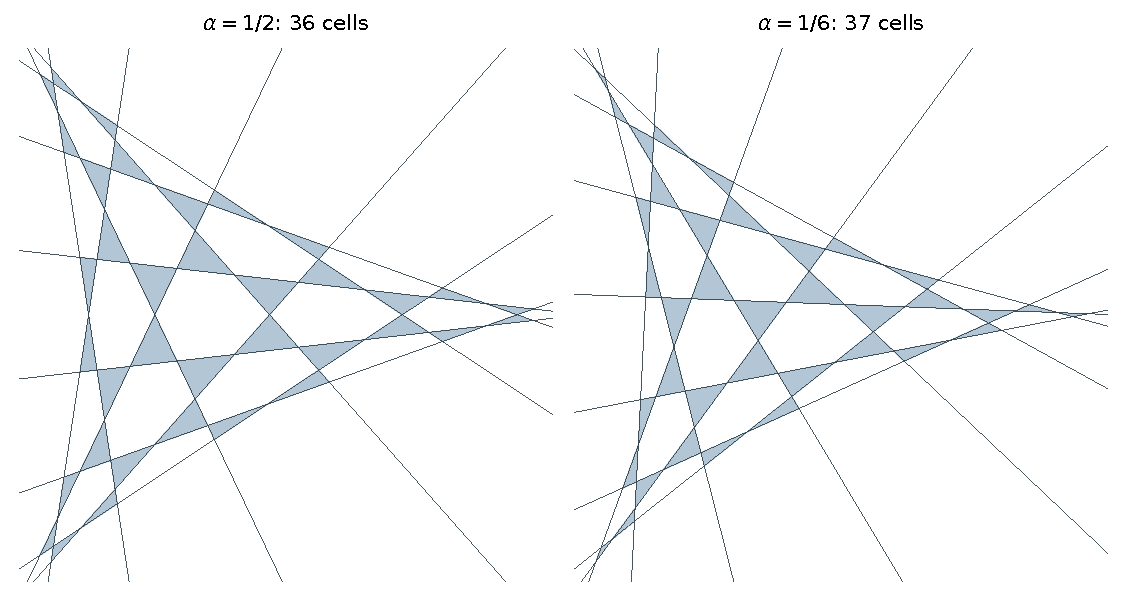
\includegraphics[width=0.9\linewidth]{phase-family.pdf}
\caption{New rational-coordinate illustrations at $n=12$, obtained from the half-phase and shifted trigonometric families. Two independent exact counters certify 36 and 37 triangles in these rational proxies. The axes of each panel are rescaled independently. The real-coordinate universal theorem follows from the symbolic sign and modular arguments, independently of this illustration. The underlying family is attributed to F\"uredi and Pal\'asti.}\label{fig:phase}
\end{figure}

\subsection{Projective changes of affine chart}

The shifted count is enough for the even part of~\eqref{eq:G}. To obtain the additional odd-order gain we use exposed vertices of the half-phase arrangement. The exact coordinate map is
\begin{equation}\label{eq:projective-map}
(x,y)\longmapsto \left(\frac{x}{h-x},\frac{y}{h-x}\right),\qquad h\ne0.
\end{equation}
It replaces the line $x=h$ by the line at infinity. The transformed coefficients of $ax+by=c$ are
\begin{equation}\label{eq:line-transform}
\Phi_h(a,b,c)=(ha-c,hb,c).
\end{equation}
Unlike an affine transformation, this change can alter which projective triangular faces appear bounded. Thus counting triangles before and after the change requires an explicit sign argument.

\begin{lemma}[Exact covariance]\label{lem:projective-covariance}
If $D(\ell,m)\ne0$, then
\begin{align}
D(\Phi_h\ell,\Phi_hm)&=hD(\ell,m)(h-x_{\ell m}),\\
E(\Phi_hr;\Phi_h\ell,\Phi_hm)&=h^2E(r;\ell,m),\\
O(\Phi_hr;\Phi_h\ell,\Phi_hm)&=h^3(h-x_{\ell m})O(r;\ell,m),\label{eq:projective-sign}
\end{align}
where $x_{\ell m}$ is the abscissa of the old intersection. If the cut avoids every old vertex, the transformed arrangement has no parallel pairs. Triple nonconcurrence is preserved.
\end{lemma}
\begin{proof}
Substitute~\eqref{eq:line-transform} into the polynomial expressions in Section~\ref{sec:geometry}, expand, and cancel. Nonzero $h$ and avoidance of all $x_{\ell m}$ give the pair determinant claim, while multiplication by $h^2$ preserves a nonzero triple evaluation.
\end{proof}

The sign multiplier in~\eqref{eq:projective-sign} also gives a direct triangle-preservation rule. If $h>0$ and all vertices of a certified triangle lie to the left of $x=h$, all three multipliers are positive. If $h<0$ and its vertices lie to the right, they are again positive. At selected exposed vertices on the opposite side, the sign reverses. Carefully choosing which vertices are separated by the cut creates the extra triangles.

\begin{lemma}[One exposed vertex]\label{lem:one-cap}
For odd $n=2m+1\ge3$, a change of affine chart of the half-phase arrangement has at least $\B(n)+1$ bounded triangles.
\end{lemma}
\begin{proof}
The intersection of $\ell(x)$ and $\ell(y)$ has abscissa
\begin{equation}\label{eq:vertex-x}
X(x,y)=\cos(2x)+\cos(2y)+\cos(2x+2y).
\end{equation}
For the half-phase angles, the vertex of lines $0,n-1$ is uniquely rightmost, with abscissa $c_n=1+2\cos(\pi/n)>0$. Indeed, each of the first two cosine terms in~\eqref{eq:vertex-x} is at most $\cos(\pi/n)$ and the last is at most one; if the pair is not $(0,n-1)$, at least one necessary inequality is strict. Choose $h>0$ between all other abscissae and $c_n$.

No selected triangle of~\eqref{eq:halfphase-triples} uses the pair $(0,n-1)$: such a triple would require its middle index to be $0$ or $n-1$ modulo $n$. Hence all counted triangles are preserved by the positive multiplier rule. The additional triple $(0,m,2m)$ has, for each test line, nonnegative evaluation at the exposed vertex and nonpositive evaluations at its other two vertices before the transformation. The cut reverses exactly the exposed-vertex sign, so the transformed triple satisfies the certificate. These signs follow from~\eqref{eq:trig-oriented} by splitting the test index at $m$. The triple is absent from the old selected list, and Lemma~\ref{lem:projective-covariance} preserves simplicity. This gives one additional bounded triangle.
\end{proof}

\begin{lemma}[Two exposed vertices]\label{lem:two-caps}
For $n=6k+3$ with $k\ge1$, a change of affine chart of the half-phase arrangement has at least $\B(n)+2$ bounded triangles.
\end{lemma}
\begin{proof}
Write $n=3m$, where $m=2k+1$. The two intersections supported by $(m-1,m)$ and $(2m-1,2m)$ have common abscissa $-c_n/2$. Every other intersection has strictly larger abscissa. To verify the latter assertion, rewrite~\eqref{eq:vertex-x} as
\[
X(u,v)=2zw+2z^2-1,
\qquad z=\cos(u+v),\quad w=\cos(u-v).
\]
For nonadjacent angle indices, the cosine bounds on the discrete grid, together with completing the square in $z$, give $X>-c_n/2$. For adjacent indices, $w=\cos(\pi/n)$ and the same quadratic attains equality precisely at $u+v=2\pi/3$ or $4\pi/3$, giving the two listed pairs. The exceptional wrapping pair $(0,n-1)$ is the rightmost vertex. These exposure inequalities are proved uniformly in \lean{FurediPalastiCaps.lean}.

Choose $h<0$ strictly above $-c_n/2$ and below all other abscissae. The modular conditions~\eqref{eq:halfphase-triples} show that no counted triangle uses either exposed pair. Its vertices are therefore all to the right of the cut and its signs are preserved. The two additional support triples are
\[
(2k,2k+1,5k+2),\qquad (k,4k+1,4k+2).
\]
For each test index, substitution into~\eqref{eq:trig-oriented} gives one sign at the exposed pair and its opposite weak sign at the other two vertices. The negative cut reverses exactly the exposed-vertex multiplier in each case, establishing the transformed certificates. The two triples are distinct and neither satisfies the old selection residues. Simplicity follows from Lemma~\ref{lem:projective-covariance}. Appending both triples to the retained list proves the claim.
\end{proof}

\begin{figure}[tbp]
\centering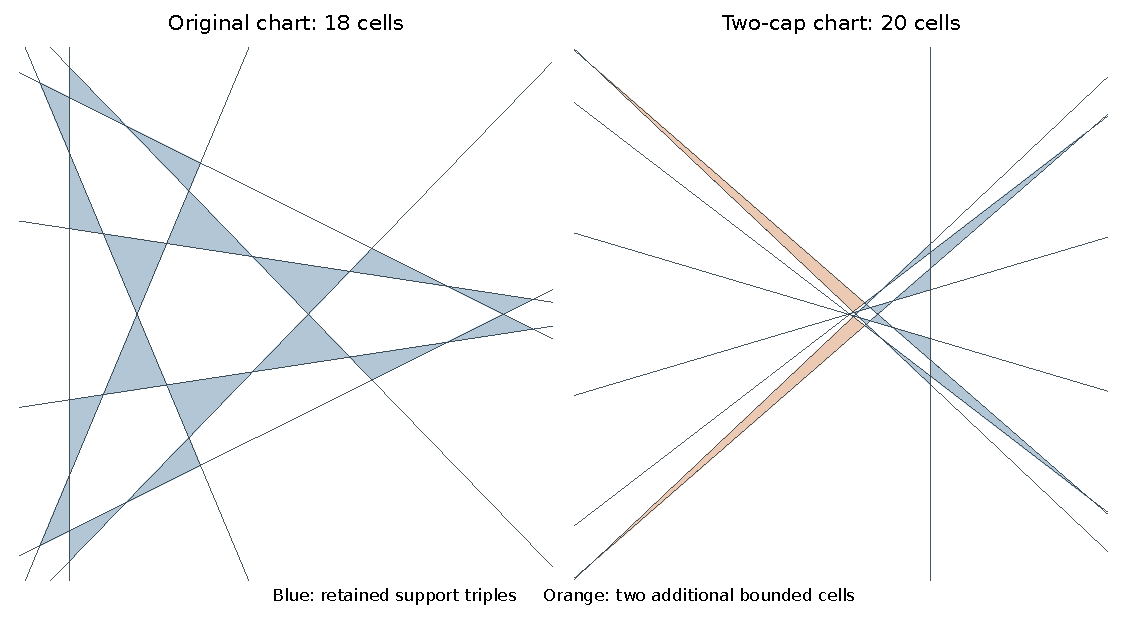
\includegraphics[width=0.95\linewidth]{affine-chart.pdf}
\caption{New exact rational illustration at $n=9$: the change of affine chart retains all 18 old triangular cells and creates two more. The resulting 20 is below the known optimum 21; this figure illustrates the uniform mechanism. Panels are rescaled independently. Both counts are checked exactly. The general proof tracks the determinant multiplier at every vertex, independently of the drawing.}\label{fig:chart}
\end{figure}

\subsection{Assembly, exact gain, and asymptotic scale}

\begin{proof}[Proof of Theorem~\ref{thm:main}]
Use Lemma~\ref{lem:shifted-count} for even $n\ge4$. For odd $n$ not divisible by three, $n(n-3)\equiv1\pmod3$, so
$\B(n)+1=\floor{n(n-3)/3}+2$; apply Lemma~\ref{lem:one-cap}. For odd multiples of three at least nine, $\B(n)=n(n-3)/3$ and Lemma~\ref{lem:two-caps} gives the same target. Three nonconcurrent lines give $\G(3)=1$, while the smaller cases have zero triangles. Each construction used is simple.
\end{proof}

\begin{corollary}[Exact improvement over the quoted baseline]\label{cor:gain}
For $n\ge4$,
\[
\G(n)-\B(n)=
\begin{cases}
1+(n\bmod2),&3\mid n,\\
n\bmod2,&3\nmid n.
\end{cases}
\]
The gains in classes $0,1,2,3,4,5\pmod6$ are respectively $1,1,0,2,0,1$.
\end{corollary}
\begin{proof}
The product $n(n-3)$ is zero modulo three when $3\mid n$, and one modulo three otherwise. Substitute these remainders in the floor and ceiling formulas.
\end{proof}

\begin{figure}[tbp]
\centering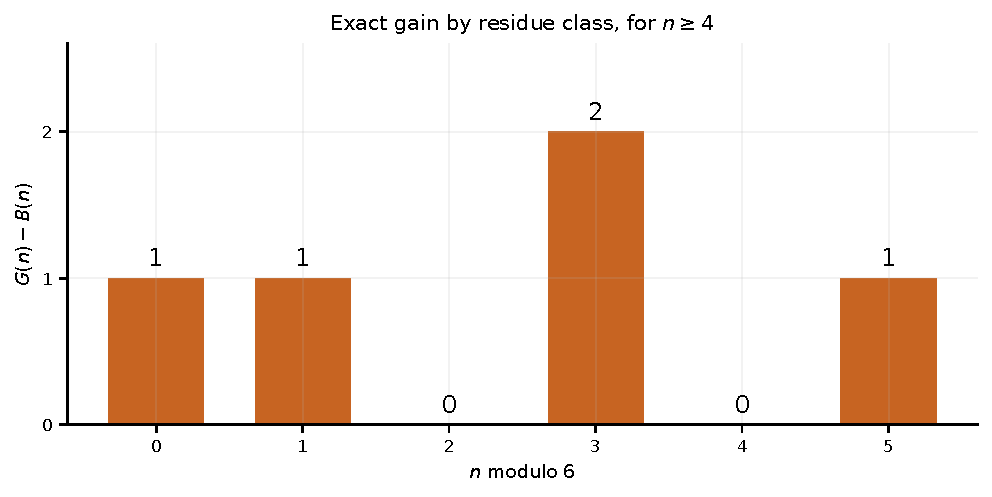
\includegraphics[width=0.88\linewidth]{residue-gains.pdf}
\caption{The exact proved gain $\G-\B$, resolved by residue class modulo six. The gain is strict on four classes; the universal statement includes arbitrarily large orders in each class.}\label{fig:residue}
\end{figure}

For comparison with the classical polynomial benchmark $\U(n)=\floor{n(n-2)/3}$, direct integer arithmetic gives, for $n\ge4$,
\begin{equation}\label{eq:gap}
\U(n)-\G(n)=\floor{\frac n3}+\mathbf1_{n\equiv2\ (3)}-1-(n\bmod2).
\end{equation}
This comparison is arithmetic. Section~\ref{upper:simple-actual} now formalizes the classical simple upper theorem; unrestricted attribution remains external. The deficit is still of order $n$, and sharper bounds or special constructions apply at some orders.

\begin{figure}[tbp]
\centering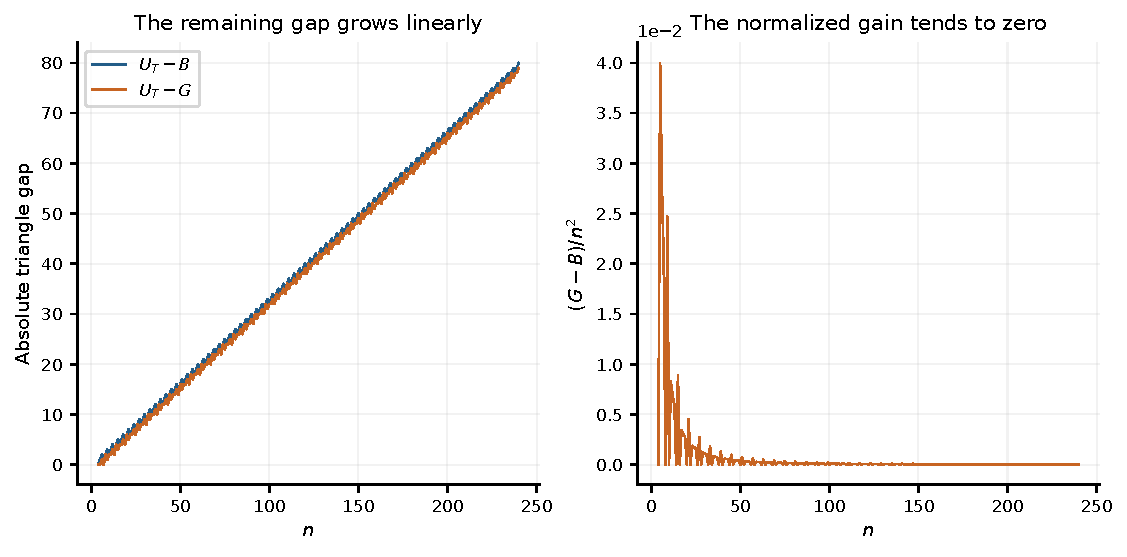
\includegraphics[width=0.94\linewidth]{normalized-gap.pdf}
\caption{Deficit and normalized growth computed from the proved formulas. The constant improvement is visible in the deficit, while both general lower formulas have the same leading quadratic and linear terms. The polynomial is the classical benchmark, now also formalized for simple arrangements; its numerical upper bound is not new.}\label{fig:normalized}
\end{figure}

The outcome is an unconditional affine theorem, stronger than the quoted baseline at infinitely many orders. Its numerical first priority remains a separate literature question. The construction gives a witness for each $n$; it does not provide an operation that adds one line to every preceding optimal witness.

\section{Individual cases, finite enhancements, and provenance}\label{sec:finite}

\subsection{The March values and their present verification}

The three finite inequalities associated with the author's early extension work are
\begin{equation}\label{eq:march-three}
\K(28)\ge238,\qquad \K(30)\ge275,\qquad \K(34)\ge357.
\end{equation}
Each now has an exact simple-arrangement certificate, so the same inequalities hold for $\Ks$. Their present validity is independent of the unproved recurrence in the original March manuscript. The certificates give actual lines and complete checked triangle lists, not only numerical consequences of an extension hypothesis.

The current OEIS table associates the name Zarzuelo with these entries~\cite{oeisA006066,zarzuelo2026}. Attribution in an index and first discovery are different questions. The earlier literature already contains matching constructions or consequences for some of these counts; the literature review records these overlaps. The claims made here are the documented attribution trail, the independently verified witnesses, and their place in the author's extension program. No new priority claim is inferred from the absence of a value from a particular online table.

\begin{figure}[tbp]
\centering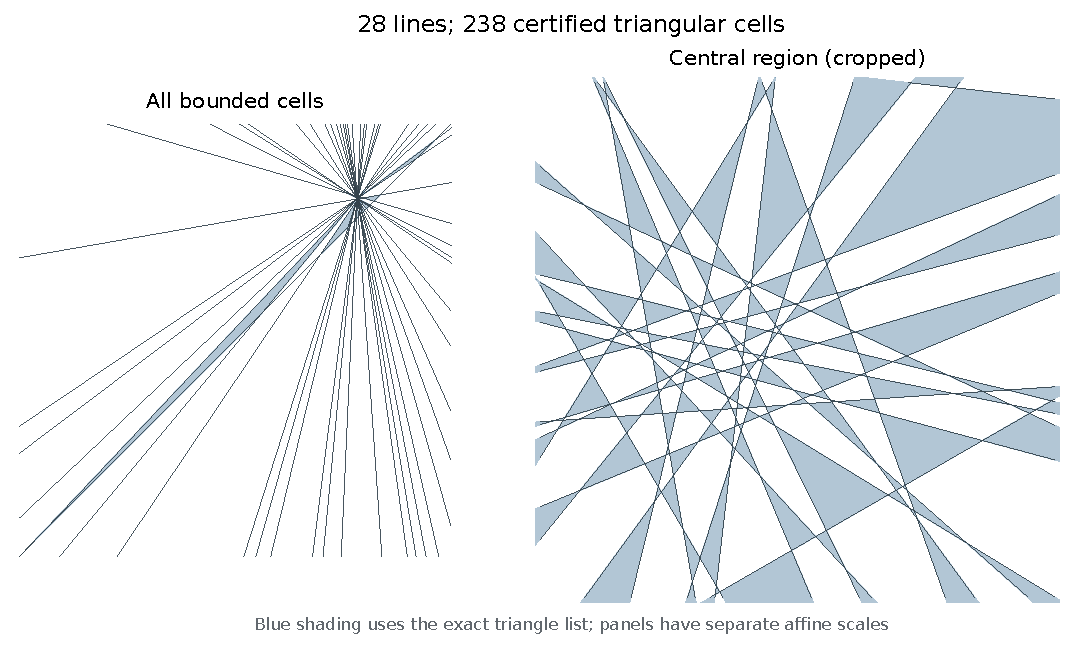
\includegraphics[width=0.96\linewidth]{historical-28.pdf}
\caption{The retained exact 28-line witness with 238 certified triangles. This is a new rendering of the saved coordinates associated with the earlier extension program. The marked zoom, where present, is an enlargement of the same arrangement; it does not add or remove lines from the certificate. The picture illustrates a lower bound, while the exact sign tests establish it.}\label{fig:historical28}
\end{figure}
\begin{figure}[tbp]
\centering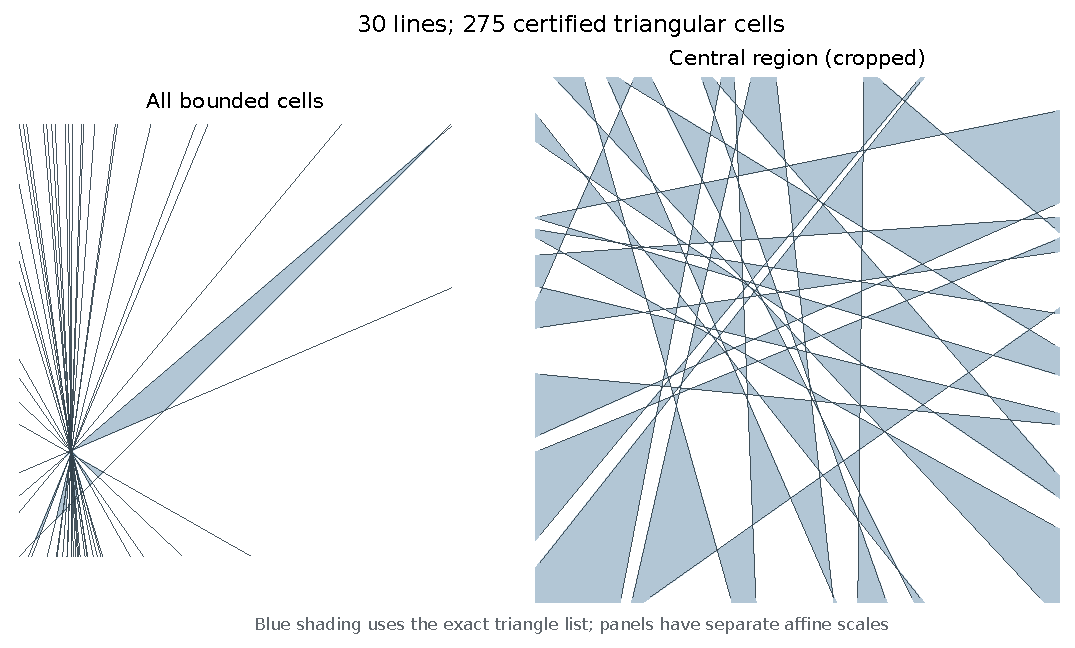
\includegraphics[width=0.96\linewidth]{historical-30.pdf}
\caption{The retained 30-line witness with 275 certified triangles, rendered from its exact coordinates. The count has prior literature overlap and is not asserted to be a new numerical record. The complete witness remains in the catalog even though the historical general extension proof was incomplete.}\label{fig:historical30}
\end{figure}
\begin{figure}[tbp]
\centering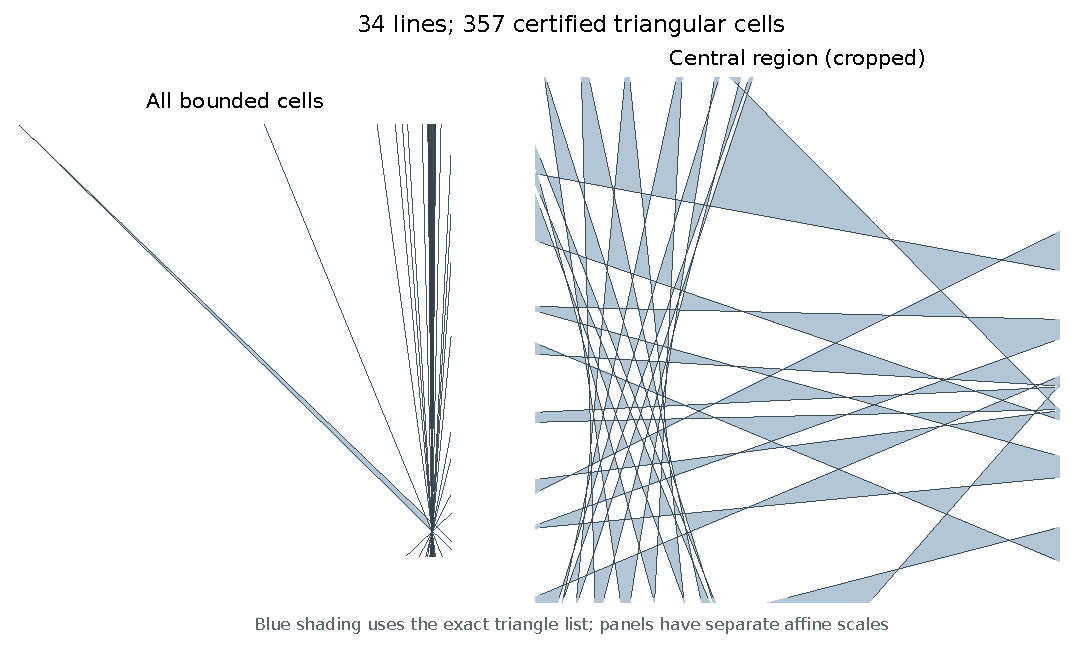
\includegraphics[width=0.96\linewidth]{historical-34.pdf}
\caption{The retained 34-line witness with 357 certified triangles. Original plotting of the certificate makes the finite conclusion inspectable independently of the claimed universal extension. The construction input and earlier matching literature are credited separately.}\label{fig:historical34}
\end{figure}

The original inventory also listed outputs for every order from 3 through 60, together with larger cases at 99 and 195. Some were direct certificates, some were numerical consequences of a boundary-defect argument, and many were weaker than an already available construction. Appendix~\ref{app:historical} preserves that inventory as history. The current certificate aliases independently retain its numerical inequalities; a label inherited from the old table is not used as a present formal-proof status.

\subsection{Materialized improvements from the phase and chart construction}

Table~\ref{tab:finite-refinement} records simple rational witnesses promoted during the last construction phase. Each listed new count is supplied by the universal theorem and also realized by an independently checked finite coordinate file. This double presentation is useful: the theorem proves all orders, while the coordinates support visualization and further exact searches.

\begin{table}[tbp]
\centering
\begin{tabular}{@{}rrrr@{}}
\toprule
$n$ & Earlier retained count & Current simple count & Increase\\
\midrule
39&469&470&1\\
47&690&691&1\\
48&720&721&1\\
51&817&818&1\\
53&884&885&1\\
54&918&919&1\\
55&954&955&1\\
59&1102&1103&1\\
60&1140&1141&1\\
99&3169&3170&1\\
195&12481&12482&1\\
\bottomrule
\end{tabular}
\caption{Changes relative to this project's previous retained witnesses, not a table of first discoveries or global record improvements. ``Simple'' is certified for every current coordinate witness in this table.}\label{tab:finite-refinement}
\end{table}

In particular, the earlier additional-line values $39:469$, $51:817$, $99:3169$ and $195:12481$ are now exceeded by $\G$ itself. Their finite correctness survives, but those numbers are not distinctive of the additional-line family. Historical evidence is retained rather than deleted when a stronger construction is found.

\subsection{The 44-line simple case}

The exact exterior extension of the retained 43-line arrangement creates 21 triangles while preserving its 587 old triangles. Both exact counters and the Lean certificate give a simple 44-line arrangement with 608 triangles. Blanc's classical simple upper bound at this order is also 608~\cite{blanc2011}. Both inequalities are now formally supported, giving
\begin{equation}\label{eq:44-simple}
\Ks(44)=608.
\end{equation}
The finite Lean certificate supplies the lower inequality, and
\sourcefile{Kobon/UpperEvenSimpleOptimality.lean}{\lean{UpperEvenSimpleOptimality}}
supplies the simple upper inequality. Equation~\eqref{eq:44-simple} is
their immediate numerical corollary, not a separate maximality wrapper.
It neither establishes $\K(44)=608$ for unrestricted arrangements nor
claims first discovery of this numerical value.

This example shows why upper-bound scope belongs next to the numerical statement. A simple witness can establish a classical lower bound, but a simple upper theorem cannot by itself close the classical problem.

\subsection{External records and independently checked inputs}

The updated catalog incorporates exact gallery witnesses from Parpalak and Utkin at
\[
8:15,\ 14:54,\ 20:117,\ 26:204,\ 32:315,\ 36:402,\ 38:450,\ 42:553,\ 46:667,\ 50:792.
\]
These are constructions or coordinate sources of the cited researchers, not newly discovered values in this project. The eight-line value has older priority; the modern gallery is the source of the checked coordinates. The public source snapshot and the formal certificate index preserve the provenance~\cite{parpalakutkin2026,oeisA006066}.

All fifteen of Maiorana's supplied 14-line arrangements with 54 triangles were independently checked and promoted as finite certificates~\cite{maiorana2026}. Fourteen have two triple points and one has four. Their source license and immutable commit are retained. These witnesses are a particularly useful warning against conflating simple and nonsimple arrangements: removing a multiple intersection by a small perturbation need not preserve the full triangle count. Section~\ref{exp:section} reports the exact resolution experiments.

The two source snapshots used for these imports are Maiorana commit
\nolinkurl{e47c7cfd9661e54d29befb83118bf83d5f804028} and gallery commit
\nolinkurl{feae4f5571a988a3ed45bd26a36259ebb7d7d3d2}. Their mathematical attribution is attached to each source record even when a new Lean wrapper or new figure is generated here.

\subsection{The finite envelope and the complete tables}

\begin{proposition}[Retained all-order envelope]\label{prop:envelope}
Let $C(n)$ be the maximum count in the finite catalog at order $n$, or zero if that order is absent. Then $\K(n)\ge\Lbound(n)=\max\{\G(n),C(n)\}$ for every $n$. In the frozen release, $\Lbound(n)=\G(n)$ for every $n>195$.
\end{proposition}
\begin{proof}
When $C(n)\le\G(n)$, use Theorem~\ref{thm:main}. Otherwise choose a certificate attaining the finite maximum and apply Proposition~\ref{prop:finite-sound}. No coordinate certificate in this release has order greater than 195. Larger computational witnesses discussed later have not been silently added to the Lean catalog.
\end{proof}

The formal definition is {\small\texttt{Universal.bound = max Universal.baseline AllN.bound}}. Since $\G\ge\B$, it equals the expression in Proposition~\ref{prop:envelope}; the older \lean{AllN} layer preserves the previous finite-envelope theorem. This makes comparisons reproducible without rewriting the historical construction history.

\begin{figure}[tbp]
\centering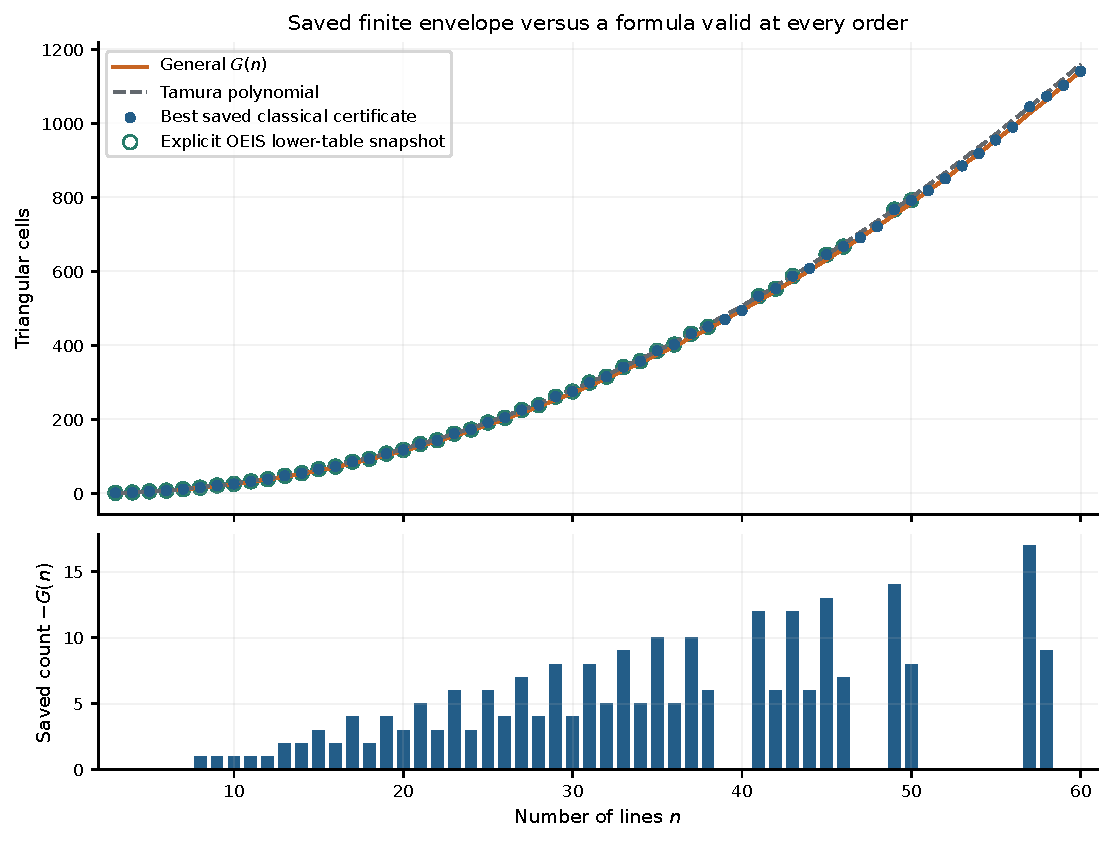
\includegraphics[width=0.96\linewidth]{finite-envelope.pdf}
\caption{The strongest saved simple and classical coordinate counts, compared with the uniform formula and the polynomial upper benchmark. External witnesses retain their attribution. A marker above $\G$ is a finite enhancement of the general formula, not automatically an original record.}\label{fig:finite-envelope}
\end{figure}

Appendix~\ref{app:finite-table} gives the best saved simple and classical values from 3 through 60. Appendix~\ref{app:catalog} lists all 138 certificate identities, including repeated orders and weaker checkpoints. Appendix~\ref{app:historical} gives the older author-output inventory. Together these tables prevent three common confusions: a retained output is not necessarily the best available value; a missing OEIS row is not proof of novelty; and an exact count for one arrangement is not automatically the extremal value $\K(n)$.

\section{Exterior extensions: the March proposal and its precise replacement}
\label{ext:section}

The starting point of this project was the March 2026 proposal that an odd
Kobon arrangement could always be extended with the gain
\begin{equation}
  \K(2m+2)\geq \K(2m+1)+m.
  \label{ext:march}
\end{equation}
The proposal was presented in \cite{zarzuelo2026} and subsequently described
as an iterative rule in \cite{handwiki2026}.  The preserved March source is
important evidence of the development of the idea, but is not a completed
proof of \eqref{ext:march}: its Lean file contains eight proof placeholders,
including the extension assertion.  The present work replaces the informal
alternating-segment argument by an actual geometric extension theorem and
identifies exactly which additional counting hypothesis yields the desired
gain.  Independently verified finite bounds are retained regardless of the
status of that original argument.

The later OEIS attribution at orders 28, 30, and 34 is evidence of the
proposal's reception, rather than a proof of numerical
priority~\cite{oeisA006066}.  In particular, the BBL table already records
the straight-line value $30:275$.  The perfect 33-line input belongs to
the family of Forge and Ram\'irez Alfons\'in~\cite{forge1998}; applying the
exterior extension stated by BBL gives $34:357$~\cite{bbl2008}.
The historical attribution, the validity of a finite count, and the
novelty of a general extension theorem are therefore assessed separately.

Two distinctions are essential.  A recurrence for maxima need not extend
\emph{every} arrangement attaining a given count, and a construction for one
odd-to-even step need not admit repeated full-gain extensions.  Throughout
this section the geometric hypotheses concern simple affine arrangements;
consequently their conclusions give lower bounds for both $\Ks$ and $\K$,
but nonsimple witnesses for $\K$ cannot automatically be substituted into
the hypotheses.

\subsection{A geometric theorem from explicitly visible pairs}

Write an old line as $L_i=\{p:\ell_i(p)=0\}$, with $\ell_i$ affine, and let
$A=\{L_0,\ldots,L_{n-1}\}$ be simple.  A linear functional $w$ is
\emph{admissible} if it is nonzero on every old line direction.  At
$p_{ij}=L_i\cap L_j$, choose the direction vectors $u_i,u_j$ on the two
supports so that $w(u_i)=w(u_j)=1$.  The following criterion uses only the
old arrangement.

\begin{definition}[Visible pair]
\label{ext:visible}
The pair $\{i,j\}$ is visible from $w$ if, for every old affine equation
$\ell_k$, the three real numbers
\[
  \ell_k(p_{ij}),\qquad D\ell_k(u_i),\qquad D\ell_k(u_j)
\]
have one common weak sign: either all are nonnegative or all are
nonpositive.  Here $D\ell_k$ denotes the linear part of $\ell_k$.
\end{definition}

Geometrically, the two increasing-$w$ rays bound an unbounded empty wedge.
The algebraic definition is convenient because it gives the required
half-plane inequalities directly, without assuming that a future triangle
already exists.

\begin{theorem}[Verified exterior realization]
\label{ext:realization}
Let $A$ be a simple arrangement of $n$ real affine lines, let $\mathcal T$
be a set of $T$ distinct triangular cells of $A$, and let $\mathcal V$ be
a set of $c$ distinct pairs visible from an admissible $w$.  If
\[
  H>\max_{i<j}w(p_{ij}),
\]
then adjoining $L=\{p:w(p)=H\}$ produces a simple arrangement containing
all triangles in $\mathcal T$ and at least $c$ further triangles.  In
particular, $\Ks(n+1)\geq T+c$.
\end{theorem}

\begin{proof}
Admissibility excludes a parallel old line, and the strict height
inequality excludes every old vertex from $L$.  Thus simplicity is
preserved.  Every old triangle lies in the convex hull of its vertices,
strictly below the level $H$, and survives unchanged.

For a visible pair, the new vertices on its two supports are
\[
 p_{ij}+(H-w(p_{ij}))u_i,
 \qquad p_{ij}+(H-w(p_{ij}))u_j.
\]
At either vertex an old affine equation has the form
\[
 \ell_k(p_{ij})+(H-w(p_{ij}))D\ell_k(u).
\]
The second coefficient is positive.  Definition~\ref{ext:visible}
therefore puts all three vertices in one closed half-plane of each old
line.  The new line is itself a supporting side, and the triangle is
nondegenerate because the old intersection lies strictly below it.  No
arrangement line cuts its interior.  Different old pairs give different
support triples, and every new triple uses $L$, whereas no old one does.
The two lists are consequently disjoint.
\end{proof}

This is the geometric content of \texttt{Exterior.extension}.  The theorem
is proved for arbitrary real coefficients and either parity, with no
assumption about a future triangle count.  An explicit formal height is
\[
  H=1+\sum_{\substack{i,j<n\\i\ne j}}|w(p_{ij})|,
\]
so existence of a sufficiently distant line is part of the construction.
The proof uses the standard Lean logical axioms and no finite native
evaluation.  What it does \emph{not} supply is a universal lower bound of
$\lfloor n/2\rfloor$ on the number of visible pairs.

\subsection{Defect, boundary wedges, and a rule for both parities}

Let $t(A)=T$ and define the bounded-segment defect
\begin{equation}
 d(A)=n(n-2)-3T.
 \label{ext:defect}
\end{equation}
There are $n(n-2)$ elementary bounded segments.  A segment can support at
most one triangular cell: its endpoints determine the two other supports,
and their intersection lies on at most one side of the segment.  Thus
$d(A)$ counts the unused bounded segments.  Let $b(A)$ count the unbounded
two-sided cells, called wedges below.

\begin{lemma}[Boundary charging]
\label{ext:charging}
For a simple arrangement of $n\geq3$ lines,
\[
  3\leq b(A)\leq n,\qquad b(A)+d(A)\geq n.
\]
\end{lemma}

\begin{proof}
The arrangement has $2n$ free rays.  A wedge pairs two such rays at their
common endpoint, and each free ray belongs to at most one wedge.  An
unpaired ray on $L$, ending at $p=L\cap M$, meets an interior vertex of
$M$.  The two bounded elementary segments of $M$ incident to $p$ cannot
both support triangles: both triangles would also use the unique bounded
segment of $L$ starting at $p$.  Charge the unpaired ray to an unused
segment of $M$ at $p$.  Each unused segment receives at most two charges,
one at each endpoint.  Hence $2n-2b\leq2d$.  This also proves $b\leq n$.
Finally, the convex hull of all finite vertices has at least three
vertices.  Both supports at a hull vertex have free outgoing rays, which
give a wedge.  Distinct hull vertices give distinct wedges.
\end{proof}

Order the $2n$ oriented line directions cyclically.  The two directions
of a wedge are consecutive: a line direction strictly inside that sector
would force a line to enter the wedge and cross a free boundary ray.
Write $B\subset\mathbb Z/(2n)$ for the wedge-start indices.  Define
\begin{equation}
 c_j=\bigl|B\cap\{j,j+1,\ldots,j+n-2\}\bigr|,
 \qquad C(A)=\max_j c_j.
 \label{ext:profile}
\end{equation}
The $n$ directions on which an admissible $w$ is positive form one
consecutive block, and every such block occurs for some normal sector.
An exterior line closes precisely the wedges whose two rays lie in this
block.  Consequently $C(A)$ is the exact largest exterior gain and
\begin{equation}
 \sum_{j=0}^{2n-1}c_j=(n-1)b(A),\qquad
 \left\lceil\frac{(n-1)b(A)}{2n}\right\rceil
 \leq C(A)\leq\left\lfloor\frac n2\right\rfloor.
 \label{ext:average}
\end{equation}
The sum follows by counting the $n-1$ blocks containing a fixed wedge.
The upper bound follows because complete wedge pairs use disjoint rays
in a block of $n$ rays.

\begin{theorem}[Boundary-defect extension]
\label{ext:defect-theorem}
For a simple $n$-line arrangement with $n\geq3$ and $T$ triangles, an
exterior line preserves the old triangles and gives at least
\begin{equation}
 T+g(n,T),\qquad
 g(n,T)=\left\lceil\frac{n-1}{2n}
       \max\{3,\,3T-n(n-3)\}\right\rceil
 \label{ext:g}
\end{equation}
triangles.  Thus, for either parity,
\[
 \Ks(n)\geq T\quad\Longrightarrow\quad
 \Ks(n+1)\geq T+g(n,T).
\]
\end{theorem}

\begin{proof}
Lemma~\ref{ext:charging} gives
$b(A)\geq\max\{3,n-d(A)\}$.  Substitute into
\eqref{ext:average} and apply Theorem~\ref{ext:realization}.  If $T$ is
only a lower bound, the witness has some count $T'\geq T$; the right side
of \eqref{ext:g} is nondecreasing in $T$, which gives the stated
maximum-function implication.
\end{proof}

\begin{remark}[Formal scope and attribution]
\label{ext:defect-scope}
Theorem~\ref{ext:defect-theorem} and its formula were already stated with
a manuscript proof in the 3 October edition. The 5--6 October development
completes the actual geometric Lean proof. For any finite injective
certified triangle family, \lean{OpenMathSimpleBoundary} extracts each
line's first and last real intersections. If $A$ counts vertices terminal
on exactly one line and $b$ those terminal on both, then
$A+2b=2n$, $A\le2U$, and $d=U$. A single-terminal vertex has three
bounded incident segments. The incident used degree is even, so at
least one is unused; its endpoint charge proves the budget. These are
\proofref{Kobon/OpenMathSimpleBoundary.lean}{454}{\lean{certificate_double_terminal_budget}}
and \proofref{Kobon/OpenMathSimpleBoundary.lean}{467}{\lean{certificate_boundary_defect}}.

Actual outward tangents have constant affine signs against every old
transverse line. Their positive normal projections imply the original
\lean{Exterior.VisiblePair} predicate. Normal charts, critical-root
ordering, sector samples and a finite double count prove that each
double-terminal vertex is selected by exactly $n-1$ of $2n$ normal
choices. A maximum projected vertex in each normal direction supplies
the minimum resource $b\ge3$. The endpoint
\proofref{Kobon/OpenMathEveryOrderExtension.lean}{45}{\lean{successor}}
therefore has no ray-order, visibility or charging oracle as a premise.
It uses only the standard logical axioms.

Exterior successors from perfect odd arrangements are already described
by BBL, and Blanc supplies individual deficit-two examples
\cite{bbl2008,blanc2011}. The general deficit-dependent scope and its
formal extraction are distinguished from those known cases. This
edition's advance over the preceding paper is completed formal linkage
and iteration, rather than first appearance of formula~\eqref{ext:g}.
Priority of the broader quantitative statement remains subject to review.
\end{remark}

\begin{proposition}[Closed gain formula and indefinite iteration]
\label{ext:actual-iteration}
For $n\ge3$ and a supplied simple lower count $T$, write
$\delta=n(n-2)-3T$. The gain in \eqref{ext:g} equals
\begin{equation}
 g(n,T)=\min\left\{\floor{n/2},
       \ceil{\frac{\max\{3,\max\{0,n-\delta\}\}}2}\right\}.
 \label{ext:closed-gain}
\end{equation}
Set $T_0=T$ and $T_{k+1}=T_k+g(n+k,T_k)$. Then for every $k\ge0$
there is a simple real arrangement of $n+k$ lines with at least $T_k$
triangles. If $n\ge4$, then $T_k\ge T+2k$.
\end{proposition}
\begin{proof}
The integer ceiling in \eqref{ext:g} simplifies to
\eqref{ext:closed-gain}; the minimum accounts for the maximum possible
number of disjoint ray pairs in a normal block. This exact arithmetic
identity is proved in
\proofref{Kobon/OpenMathExtensionFormula.lean}{56}{\lean{closed_form_successor}}.
Apply the actual successor repeatedly: each output is again simple and
has the larger order required by the next application. Induction gives
the stated sequence, in
\proofref{Kobon/OpenMathEveryOrderExtension.lean}{82}{\lean{infinite_quantitative_extension}}.
For $n\ge4$, \eqref{ext:closed-gain} is at least two; summing yields the
last inequality. This is an existence theorem for every finite iteration
length and does not require a fixed normal direction throughout the chain.
\end{proof}

\begin{corollary}[Full gain for an odd saturated input]
\label{ext:odd-full}
If a simple arrangement of $2m+1$ lines has defect at most two, an exterior
line creates exactly $m$ additional triangles.  In particular, this
applies to every simple odd arrangement attaining
$\lfloor n(n-2)/3\rfloor$.
\end{corollary}

\begin{proof}
The wedge count is at least $2m-1$.  If all $4m+2$ direction sectors had
gain at most $m-1$, then
\[
 2m(2m-1)\leq 2m b(A)=\sum_jc_j
 \leq(4m+2)(m-1)=2m(2m-1)-2,
\]
a contradiction.  Equation~\eqref{ext:average} bounds the gain above by
$m$.  The segment-count upper bound at odd $n$ leaves defect zero or two.
\end{proof}

For an even input $n=2m$, the sufficient condition $b(A)\geq2m-1$ likewise
forces gain $m$, because $(2m-1)^2>4m(m-1)$.  In either parity the exact
criterion is the finite condition $C(A)=\lfloor n/2\rfloor$.
There is no claim that every even or odd maximum has this boundary
profile. Iterating \eqref{ext:g} is now fully formalized and supplies a
weaker lower-bound rule from any simple seed. The full-gain corollary and
its simple optimality consequence are also completed in
\sourcefile{Kobon/OpenMathOptimalSuccessor.lean}{\lean{OpenMathOptimalSuccessor}}.

\subsection{What fails in indefinite full-gain exterior iteration}

The March argument made the number of new triangles follow from an
alternation assertion after placing a line far from all old vertices.
Distance proves preservation; it does not prove emptiness for half the
new segments.  For example, the five lines $y=ix+i^2$, $i=0,\ldots,4$,
have three triangles, and adding $y=x/2+100$ creates only one further
triangle.  These counts are checked by exact certificates.  This refutes
that unqualified step of the argument, without refuting a better choice
of line or an inequality about maxima.

A stronger obstruction concerns every chain of exterior additions.
Write $b_r$ for its wedge count and $c_r$ for the gain at step $r$.
Closing $c_r$ wedges consumes those wedges.  No new free ray can appear
at an old vertex, and a wedge at a new vertex must use one of the two
free rays of the newly added line.  Therefore
\begin{equation}
 b_{r+1}+c_r\leq b_r+2,
 \qquad
 \sum_{j<r}c_j\leq b_0+2r-b_r\leq b_0+2r-3.
 \label{ext:budget}
\end{equation}
The accumulated exterior gain is at most linear in the number of steps.
The accumulated gains $\lfloor n/2\rfloor$ are quadratic, so an infinite
chain of such full-gain exterior steps is impossible.  The numerical
contradiction is formalized in
\texttt{Iteration.no\_infinite\_full\_gain\_budget}. The universal
interpretation of the consumed-wedge budget is a manuscript geometric
argument; the completed quantitative successor does not assume that
full gains or one fixed boundary profile persist.

\begin{table}[tb]
\centering
\small
\begin{tabular}{rrrrr}
\hline
Input order & Triangles & Wedges & Best exterior gain & Requested gain\\
\hline
49&767&47&24&24\\
50&791&24&23&25\\
51&814&3&2&25\\
52&816&3&2&26\\
53&818&3&2&26\\
\hline
\end{tabular}
\caption{One exact greedy exterior chain from the attributed 49-line
input.  Every direction sector was counted with rational arithmetic.
These are capacities of the displayed arrangements, not upper bounds
for $\K$ or $\Ks$ at the corresponding orders.}
\label{ext:49-table}
\end{table}

Table~\ref{ext:49-table} records the motivating test from $49:767$.
The obstruction is independent of the greedy tie break: two exterior
gains $24$ and $25$ from this seed would imply
\[
 b_2\leq47+4-24-25=2,
\]
contrary to $b_2\geq3$.  The five finite profile maxima have a checked
Lean arithmetic certificate; their identification with the saved
coordinates is supplied by the exact geometry program.  A reconstruction
between steps or an interior insertion could evade this boundary budget,
so it does not disprove the proposed recurrence for maxima.

\begin{figure}[tb]
\centering
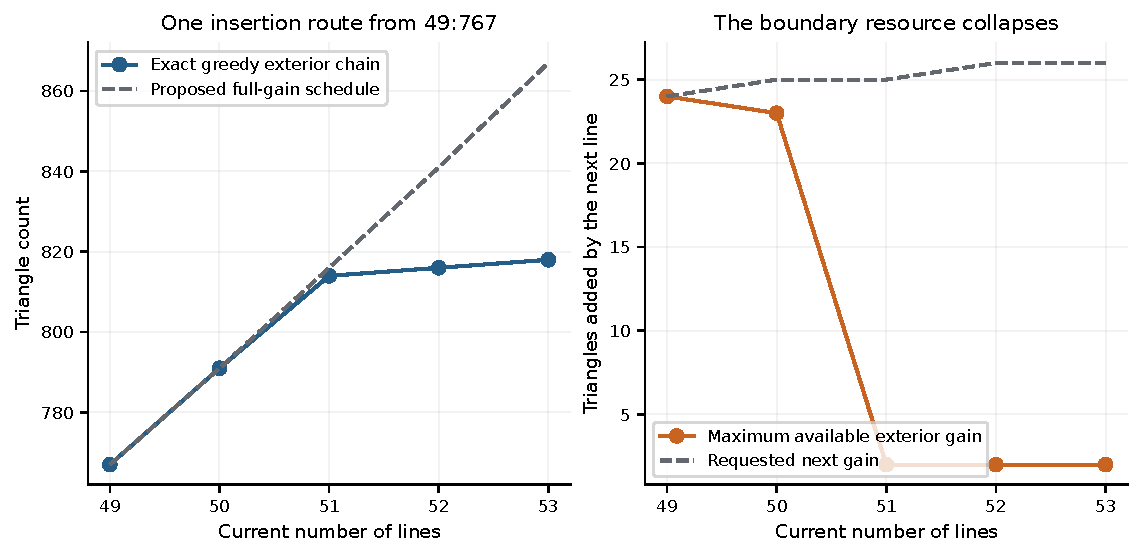
\includegraphics[width=0.88\linewidth]{figures/successor-49-resource.pdf}
\caption{The boundary resource in the particular exact 49-line chain.
The sharp drop in available wedges explains why its first full-gain
extension cannot be repeated with the requested next gain.  The plotted
capacities concern this chain only.}
\label{fig:successor}
\end{figure}

\subsection{A conditional recurrence and an unconditional numerical bound}

For any integer-valued function $F$, assume
\begin{equation}
 F(n+1)\geq F(n)+\lfloor n/2\rfloor\qquad(n\geq s).
 \label{ext:full-step}
\end{equation}
Summation, including both parity cases, gives the fully checked arithmetic
implication
\begin{equation}
 F(n)\geq F(s)+
 \left\lfloor\frac{(n-1)^2}{4}\right\rfloor-
 \left\lfloor\frac{(s-1)^2}{4}\right\rfloor
 \qquad(n\geq s).
 \label{ext:conditional-closed}
\end{equation}
The hypothesis \eqref{ext:full-step} remains explicit in the formal
theorem.  Substituting $s=49$ and $F(49)=767$ yields the numerical target
\begin{equation}
 Q_{49}(n)=\left\lfloor\frac{(n-1)^2}{4}\right\rfloor+191.
 \label{ext:49-target}
\end{equation}

There is now a separate unconditional Lean theorem
\begin{equation}
 \K(n)\geq Q_{49}(n)\qquad(n\geq49),
 \label{ext:49-unconditional}
\end{equation}
proved using the saved witnesses at 49 and 50 and the classical all-order
baseline thereafter.  Indeed, for $n\geq51$,
\[
 \frac{n(n-3)}3-\frac{(n-1)^2}4-191
 =\frac{n^2-6n-2295}{12}\geq0,
\]
with equality at $n=51$ and an increasing numerator beyond it.  Rounding
gives $\B(n)\geq Q_{49}(n)$.  This proves the desired numerical formula
without constructing a nested full-gain chain.  The stronger all-order
bound $\G$ and the finite envelope elsewhere in this paper also dominate
it.

For comparison, direct iteration of the defect rule
$T_{n+1}=T_n+g(n,T_n)$ from $49:767$ guarantees
$50:791$, $51:803$, $52:805$, and $60:821$.
The stronger target \eqref{ext:49-target} gives $51:816$, $52:841$, and
$60:1061$.  These are different constructions and different assertions.
The completed numerical theorem does not retrospectively prove the
March extension claim, and the failure of its proposed exterior
iteration does not invalidate the completed numerical theorem.

\section{Compatible seeds, geometric doubling, and sparse families}
\label{fam:section}

The second extension mechanism inserts a whole collection of lines near
a distinguished support.  It belongs to Bartholdi, Blanc, and Loisel
(BBL)~\cite{bbl2008}; it is fundamentally different from the one-line
exterior operation of Section~\ref{ext:section}.  The present work supplies
explicit compatible seeds, a recursively closed geometric Lean proof, and
finite certificates at considerably larger orders. The 2 October release
completed both the odd iteration and the stronger adjacent-even family;
the 5--6 October work discharges further compatible seed interfaces.
The numerical doubling gain retains its published attribution.

\subsection{The exact one-step theorem}

Let $q=4r$ with $r\geq5$, put $\alpha=\pi/q$, and take
\begin{equation}
  0<\varepsilon<\tan(\alpha/2).
  \label{fam:epsilon}
\end{equation}
Define $q$ ordered intercepts, indexed from zero, by
\begin{equation}
 a_j=
 \begin{cases}
 \tan((j-q/2+1)\alpha),&0\leq j<q/2-1,\\
 -\varepsilon,&j=q/2-1,\\
 \varepsilon,&j=q/2,\\
 \tan((j-q/2)\alpha),&q/2<j<q.
 \end{cases}
 \label{fam:old-grid}
\end{equation}
In particular, the extreme intercepts are $-\cot\alpha$ and
$\cot\alpha$.  The two central intercepts replace the repeated zero that
would otherwise occur in this grid.

\begin{definition}[Compatible tangent-grid seed]
\label{fam:compatible}
A seed at $(q,\varepsilon)$ consists of $Y_0:y=0$ and the $q$ lines
$L_j:y=m_j(x-a_j)$, with the following properties: the arrangement is
simple; every interval $[a_j,a_{j+1}]$ on $Y_0$ supports the triangular
cell with supports $Y_0,L_j,L_{j+1}$; and the central apex
$L_{q/2-1}\cap L_{q/2}$ lies above $Y_0$.  A counted seed additionally
carries a list of distinct actual triangular cells whose length is at
least $T$.
\end{definition}

Simplicity already requires all $m_j$ to be nonzero and pairwise distinct.
The distinguished-line condition is a substantial geometric restriction,
not a consequence of having a large total count.  It is precisely why
an arbitrary optimal arrangement cannot simply be used as a repeatable
BBL seed.

\begin{theorem}[Fully verified geometric doubling]
\label{fam:doubling}
Suppose $q=4r\geq20$ and \eqref{fam:epsilon} holds.  A compatible
tangent-grid seed with at least $T$ certified triangles gives a simple
real straight-line arrangement of $2q+1$ lines with at least
\begin{equation}
  T+q^2
  \label{fam:gain}
\end{equation}
triangles.
\end{theorem}

The precise formal theorem is \texttt{BBLDoubling.doubling}.  It assumes
the actual old line equations, simplicity, each distinguished triangle,
the positive central height, and a duplicate-free triangle list.  It
does not assume a future crossing order, a list of future empty
triangles, or a triangle-count recurrence.  Its conclusion is an actual
\texttt{SimpleLowerBound}; the generic proof uses only the standard Lean
logical axioms.  The numerical doubling principle is BBL's.  The
contribution here is its completed geometric proof for these explicit
hypotheses, using the following two-parameter realization.

\begin{proof}[Geometric proof and its formal decomposition]
For $0\leq i<q$ set
\[
 \beta_i=-\frac\pi2+(i+\tfrac12)\alpha,
 \qquad b_i=\tan\beta_i.
\]
Adjoin the lines
\begin{equation}
 M_i:\quad y=\kappa g_i(\delta)(x-b_i),\qquad
 g_i(\delta)=\frac{2b_i}{1+b_i^2}+\frac\delta{b_i}
            =\sin(2\beta_i)+\delta\cot\beta_i.
 \label{fam:pencil}
\end{equation}
Choose $\delta>0$ sufficiently small and then $\kappa>0$ sufficiently
small relative to the fixed $\delta$ and the seed.  This order of choices
is part of the proof.  BBL's published construction uses explicit scales;
the qualitative two-scale statement here is established independently
by the formal crossing analysis, rather than inferred from those fixed
scales.

For two new lines put $t=b_i$ and $u=b_k$.  Their intersection has
$x$-coordinate independent of $\kappa$:
\begin{equation}
 X_{ik}(\delta)=
 \frac{2tu(t+u)}{2tu(1-tu)-\delta(1+t^2)(1+u^2)}.
 \label{fam:crossing}
\end{equation}
When $tu\ne1$, its limit is the reduced tangent
$(t+u)/(1-tu)=\tan(\beta_i+\beta_k)$, and the exact displacement is
\begin{equation}
 X_{ik}(\delta)-\frac{t+u}{1-tu}
 =\frac{\delta(t+u)(1+t^2)(1+u^2)}
 {[2tu(1-tu)-\delta(1+t^2)(1+u^2)](1-tu)}.
 \label{fam:displacement}
\end{equation}
For sufficiently small positive $\delta$ its nonzero sign is that of
$(t+u)tu$.  If $tu=1$, the crossing diverges along the specified exterior
ray as $\delta\downarrow0$; if $t+u=0$, its coordinate is exactly zero.
Thus neither exceptional case is hidden inside a continuity argument
with a vanishing denominator.

The reduced tangents, the old intercepts, the new half-grid intercepts,
and $-\varepsilon,0,\varepsilon$ determine a strictly ordered finite
system of cuts.  Equations~\eqref{fam:crossing}--\eqref{fam:displacement}
place every new--new crossing in its prescribed cut interval.  Taking
$\delta$ in the intersection of the finitely many resulting positive
neighborhoods also makes the new slope factors nonzero and distinct.
For fixed such $\delta$, each old--new intersection tends to the
corresponding old intercept as $\kappa\to0$.  Finite continuity then
realizes all the prescribed strict crossing comparisons simultaneously.
Small $\kappa$ separates old and new slopes.  Injectivity along each new
crossing row excludes new triple intersections; old simplicity excludes
the remaining ones.  This proves actual simplicity and crossing order.

The count can now be separated from trigonometry.  Treat the $q$ new lines
and $Y_0$ as $q+1$ auxiliary supports.  The integer row model places old
support $j$ at key $4j+2$.  A pair of auxiliary supports with crossing key
$z$ yields a mixed triangle with old support $j$ when
\begin{equation}
  |z-(4j+2)|<4.
  \label{fam:neighbors}
\end{equation}
Every auxiliary pair has two such old neighbors, except for at most $q$
exterior pairs, each of which has one.  Hence the number is at least
\begin{equation}
 2\binom{q+1}{2}-q=q^2.
 \label{fam:mixed-count}
\end{equation}
The row inequalities make two sides consecutive on their supports.
The two-side emptiness lemma proves that the corresponding triangle is
an actual empty cell.  The supporting triples are distinct.  Thus
\eqref{fam:mixed-count} counts genuine triangles, not merely local
crossing patterns.

It remains to preserve the seed's contribution.  An old triangle not
using $Y_0$ has a strict half-plane sign against $Y_0$; all new lines
converge to $Y_0$, so its three vertex signs persist for sufficiently
small $\kappa$.  The old triangles with a side on $Y_0$ require a different
argument.  Saturation forces consecutive old apices to have opposite
heights.  The positive central apex fixes the alternating parity.
The crossing order identifies a new cap support for each noncentral
distinguished triangle.  On both cap endpoints, every new line has the
parity-correct weak sign; strict signs against other old supports
persist by continuity.  This replaces each such old triangle by one
empty triangle with the same two old supports.  The central triangle
itself is retained.  The finite cap and noncap requirements can again
be satisfied by one common positive $\kappa$.

Finally, these $T$ retained or replaced triangles have at least two old
nonhorizontal supports, while the $q^2$ mixed triangles have two
auxiliary supports.  The supporting triples cannot coincide.  Their
union is a duplicate-free witness of length at least $T+q^2$.
\end{proof}

The recurrence preserves the certified segment deficit:
\begin{equation}
 \Delta(q,T)=q^2-1-3T,\qquad
 \Delta(2q,T+q^2)=\Delta(q,T).
 \label{fam:deficit-preserved}
\end{equation}
Here the equality concerns the transported lower count; if the output
has additional uncounted triangles, its actual defect can be smaller.
Thus doubling amplifies a compatible seed to larger orders while
preserving its certified constant deficit.  A smaller-defect seed or a
new source of additional triangles is needed to improve that deficit.

\subsection{The compatible eleven-line realization}

The useful eleven-line count is $32$, an existing result; the search
started from the Honma-based construction displayed by
Savchuk~\cite{savchuk2025}.  The additional work here is an explicit
realization compatible with the BBL grid for arbitrarily small positive
central separation.  Take $Y_0:y=0$ and
\begin{equation}
 x-v_jy=a_j,\qquad
 (v_0,\ldots,v_9)=\tfrac1{10}(15,-2,14,1,4,-4,5,-3,12,-5),
 \label{fam:seed11-slopes}
\end{equation}
where
\begin{equation}
 (a_0,\ldots,a_9)=
 (-\tan\tfrac{4\pi}{10},-\tan\tfrac{3\pi}{10},
 -\tan\tfrac{2\pi}{10},-\tan\tfrac{\pi}{10},
 -\varepsilon,\varepsilon,
 \tan\tfrac{\pi}{10},\tan\tfrac{2\pi}{10},
 \tan\tfrac{3\pi}{10},\tan\tfrac{4\pi}{10}).
 \label{fam:seed11-grid}
\end{equation}
For every $0<\varepsilon\leq10^{-5}$ the seed is simple, has at least
32 certified triangles, and has all nine distinguished triangles.
Its central slopes are $5/2$ and $-5/2$ and its central height is
$5\varepsilon/2>0$.

The stability check is finite but uniform in $\varepsilon$.  The
determinant for a triple of nonhorizontal lines is affine in the
intercepts and therefore affine in $\varepsilon$:
\[
 D_{ijk}=(a_j-a_k)v_i+(a_k-a_i)v_j+(a_i-a_j)v_k.
\]
Exact rational enclosures for the four tangent values and endpoint
sign checks certify the whole interval.  The first certificate used
outward rational interval arithmetic; the subsequent Lean theorem uses
proved trigonometric enclosures and the parametric certificate soundness
theorem.  The limit $\varepsilon=0$ is used only to bound expressions;
it is not presented as a simple arrangement.  Five visible pairs for
$w=(10,-13)$ are also proved uniformly, giving the actual exterior bound
$12:37$ by Theorem~\ref{ext:realization}.

\begin{figure}[tb]
\centering
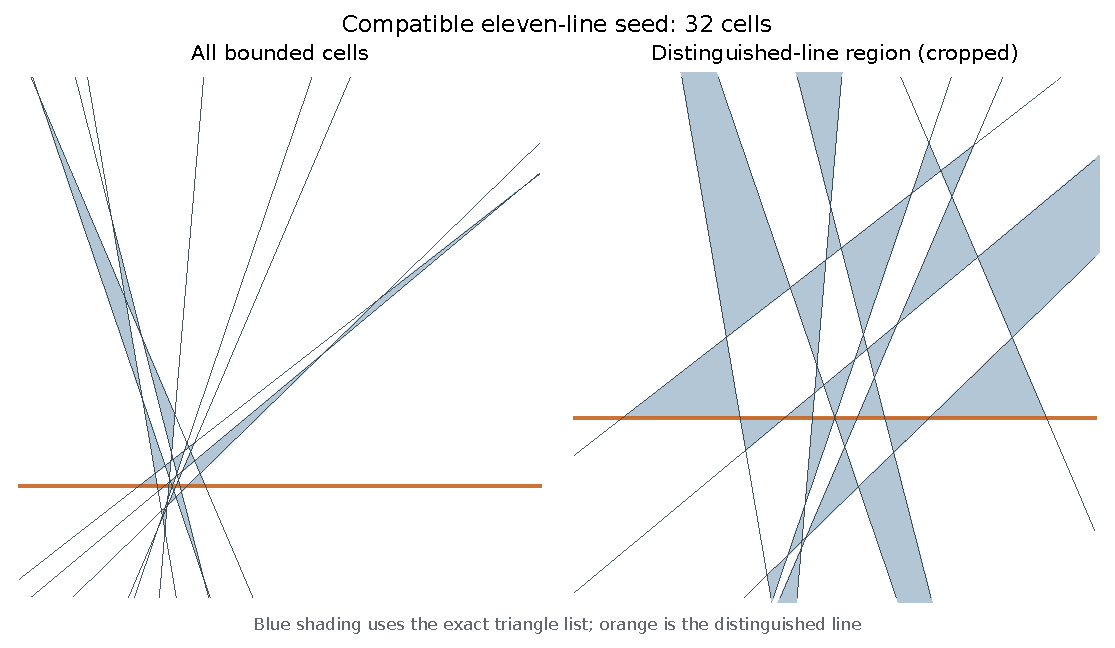
\includegraphics[width=0.88\linewidth]{figures/seed-11.pdf}
\caption{A finite rational realization of the compatible eleven-line
seed, with global and distinguished-line views.  The figure illustrates
the arrangement; the all-small-parameter
claim is certified by exact determinant and half-plane inequalities,
not by the rendering.  The count $32$ is inherited from earlier work;
the compatible realization and parameter certificate are the contribution
recorded here.}
\label{fig:seed11}
\end{figure}

\subsection{Closing the geometric invariant}

A numerical inequality after one step is insufficient for induction. The
output must again satisfy every geometric hypothesis in
Definition~\ref{fam:compatible}. The October construction returns precisely
that information. The \proofref{Kobon/BBLRecursiveSeed.lean}{11}{seed record}
contains actual slopes, a duplicate-free valid triangle list, simplicity,
every consecutive distinguished triangle, and the positive central apex.
The line labels are normalized by explicit inverse permutations; the
transport theorem preserves actual support triples and their triangle
predicates, rather than merely transporting a count.

\begin{theorem}[Closed geometric iteration]\label{fam:closed-iteration}
Fix $r\ge5$ and a counted seed size $T$. Suppose that for every sufficiently
small positive $\varepsilon$ a compatible tangent-grid seed with $4r+1$
lines and at least $T$ triangles exists. Then for every integer $t\ge0$
there is a simple arrangement of $4r\,2^t+1$ lines with at least $T_t$
triangles, where
\begin{equation}
 T_0=T,\qquad T_{t+1}=T_t+(4r\,2^t)^2,
 \qquad 3T_t+(4r)^2=3T+(4r\,2^t)^2.
 \label{fam:closed-count}
\end{equation}
At every finite depth the full seed invariant is available on some
nonempty positive parameter interval.
\end{theorem}

\begin{proof}
The geometric construction in Theorem~\ref{fam:doubling} is performed
while retaining the next distinguished triangles and the positive central
triangle. Its output intercepts, after the proved reindexing, are exactly
the tangent grid for $2r$. Simplicity and the counted list are carried in
the same witness. This is
\proofref{Kobon/BBLRecursiveSeed.lean}{61}{\lean{seed_step}}; its
coefficient identities are proved in \lean{BBLRecursiveGrid} and its
unreindexed geometric witness in \lean{BBLRecursiveWitness}.

More explicitly, let $\eta>0$ be a valid input threshold. The next seed
exists for every
\[
 0<\varepsilon<\min\{\eta,\tan(\pi/(8r))\}.
\]
The minimum is positive. For each such $\varepsilon$, the small pencil
parameters are chosen as in the one-step proof. No uniform lower bound
on these auxiliary parameters is needed. Thus the whole seed property,
including its nonempty interval, is preserved by $r\mapsto2r$.
Induction proves the first assertion and the recurrence. Multiplying
the recurrence by three and using $(2q)^2=q^2+3q^2$ proves the displayed
identity by induction. The formal results are
\proofref{Kobon/BBLInfinite.lean}{32}{\lean{uniform_iterate}},
\proofref{Kobon/BBLInfinite.lean}{46}{\lean{infinite_family}}, and
\proofref{Kobon/BBLInfinite.lean}{52}{\lean{triangleCount_identity}}.
\end{proof}

The quantifier is $\forall t\,\exists\eta_t>0\,\forall\varepsilon
\in(0,\eta_t)$, with a seed witness for each such parameter. It is not
$\exists\varepsilon>0\,\forall t$. In particular, the theorem does not
claim that a fixed drawn arrangement can be iterated with one fixed
positive gap forever. This distinction closes the earlier proof gap
without inserting an unproved compactness assertion.

The normalized 21-line seed supplies $r=5$, $T=132$ throughout
$0<\varepsilon\le10^{-5}$. Its nineteen distinguished triangles, actual
coefficient identity, and central height $5\varepsilon/2$ are proved in
\lean{BBLSeed21Normalized}. The generic theorem starts at $r\ge5$;
the separately verified eleven-line seed supplies the initial term in
the following family.

\begin{theorem}[Verified odd family]\label{fam:odd-verified}
For every integer $t\ge0$, set $q_t=10\cdot2^t$. Then
\begin{equation}
 \Ks(q_t+1)\ge T_t=\frac{100\cdot4^t-4}{3}
                    =\frac{q_t^2-4}{3}.
 \label{fam:eleven-family}
\end{equation}
\end{theorem}
\begin{proof}
For $t=0$ use the eleven-line certificate. For $t\ge1$ apply
Theorem~\ref{fam:closed-iteration} to the normalized 21-line seed at depth
$t-1$. Equation~\eqref{fam:closed-count} gives $3T_t+4=q_t^2$.
The exact formal declaration is
\proofref{Kobon/BBLVerifiedFamilies.lean}{24}{\lean{eleven_odd_family}}.
\end{proof}

The generic iteration uses only standard logical axioms. The concrete
family additionally inherits four existing native certificate checks
from its 21-line base. This is an unconditional geometric existence
theorem with an explicitly reported computation trust boundary, not a
conditional recurrence on unknown arrangements.

\subsection{Even companions and the retained boundary invariant}

The defect argument of Theorem~\ref{ext:defect-theorem} gives the weaker
ordinary mathematical consequence
\begin{equation}
 \Ks(q+2)\ge\frac{q^2-4}{3}+\frac q2-1,
 \qquad q=10\cdot2^t.
 \label{fam:even-defect}
\end{equation}
Indeed its gain is
$\lceil q(q-2)/(2(q+1))\rceil=q/2-1$. The October proof establishes the
additional visible pair at every depth, rather than extrapolating from
finite checkpoints.

A visible seed extends the preceding seed record by an admissible normal
$w=(w_x,w_y)$, a duplicate-free list of at least $V$ visible pairs, and a
rightmost old line $R$ satisfying
\[
 m_R>0,\qquad w_x+w_y m_R>0,
 \qquad x(R\cap L_i)\le a_R \quad(L_i\ne R).
\]
These are concrete line-intersection conditions. The record is
\proofref{Kobon/BBLVisibleSeed.lean}{7}{\lean{VisibleSeed}}. The generic
iteration additionally assumes $w_x>0$.

\begin{theorem}[Closed visible-boundary iteration]\label{fam:visible-iteration}
Under these uniform visible-seed hypotheses with $r\ge5$, doubling
preserves the normal and the whole visible-seed record, with
\begin{equation}
 (r,T,V)\longmapsto(2r,T+(4r)^2,V+2r).
 \label{fam:visible-step}
\end{equation}
Consequently, at depth $t$ the visible count satisfies
$V_t+2r=V+2r\,2^t$. If $V=2r$, the exterior extension yields at least
$T_t+2r\,2^t$ triangles at order $4r\,2^t+2$.
\end{theorem}

\begin{proof}
Old visible pairs avoiding $Y_0$ persist under a sufficiently small
pencil; at most one visible old pair uses $Y_0$. The new construction
supplies $r$ negative complementary pairs, $r-1$ positive
almost-complementary pairs, the pair of $Y_0$ and the rightmost new
support, and the pair of $R$ with the support at
$\beta_* =\pi/4-\alpha/2$. This supplies $2r+1$ pairs, compensating for
the possible old loss and leaving a gain of $2r$. Pair supports and
new/old tags prove that the retained list has no duplicates.

The last pair is controlled by
\[
 \cot\alpha\sin(2\beta)+\cos(2\beta)-1
   =\frac{\sin(2\beta+\alpha)}{\sin\alpha}-1.
\]
On the half-grid its unique maximum occurs at $\beta_*$, with a gap
at least $2\sin\alpha$. First shrink $\delta$ to preserve this strict
maximum, then shrink $\kappa$ to compare the actual new crossing with
all old vertices on $R$. The positivity of projected graph directions
transfers horizontal crossing order to $w$-order. The corresponding
rightmost clean ray is then established on the next grid. The finite
requirements are intersected with the eventual one-step witness, so the
same output has the old seed invariant and the new boundary invariant.

This is the geometric content of
\proofref{Kobon/BBLEvenStep.lean}{34}{\lean{canonical_visible_step}}
and \lean{BBLEvenRecursive.visible_seed_step};
\lean{BBLProjection}, \lean{BBLRightmost} and
\lean{BBLNextBoundary} supply the actual order and intersection lemmas.
Reindexing transports visibility and admissibility. The positive
parameter-interval induction is the same as for odd seeds. Summing
$V_{t+1}-V_t=2r\,2^t$ gives $V_t=V+2r(2^t-1)$. Finally apply the
proved exterior theorem to this actual visible-pair list.
\end{proof}

\begin{theorem}[Verified full-gain even family]
\label{fam:even-conditional}
For every integer $t\ge0$ and $q=10\cdot2^t$,
\begin{equation}
 \Ks(q+2)\ge\frac{q^2-4}{3}+\frac q2.
 \label{fam:even-strong}
\end{equation}
\end{theorem}
\begin{proof}
The normalized 21-line visible seed has $r=5$, $T=132$, $V=10$ and
$w=(10,-13)$. Its full rightmost-boundary and visibility hypotheses
hold uniformly for $0<\varepsilon\le10^{-5}$. Apply
Theorem~\ref{fam:visible-iteration}; the independently verified
$12:37$ witness supplies $t=0$. The unconditional declaration is
\proofref{Kobon/BBLVerifiedFamilies.lean}{51}{\lean{eleven_even_family}}.
Its dependencies include the four odd-seed native checks and two further
finite admissibility/visibility checks. No unresolved visibility
hypothesis remains in this concrete theorem.
\end{proof}

\begin{table}[tb]
\centering\small
\begin{tabular}{rrrrrl}
\toprule
$q$ & Odd order & Odd count & Even order & Even count & Family proof\\
\midrule
10&11&32&12&37&Lean existence\\
20&21&132&22&142&Lean existence\\
40&41&532&42&552&Lean existence\\
80&81&2132&82&2172&Lean existence\\
160&161&8532&162&8612&Lean existence\\
320&321&34132&322&34292&Lean existence\\
640&641&136532&642&136852&Lean existence\\
\bottomrule
\end{tabular}
\caption{The completed odd and even family. Every displayed existential
bound now follows from one general Lean theorem. This does not change
the separate verification status of previously exported coordinate files,
nor assert that these numbers exceed all literature constructions.}
\label{fam:finite-table}
\end{table}

\begin{figure}[tb]
\centering
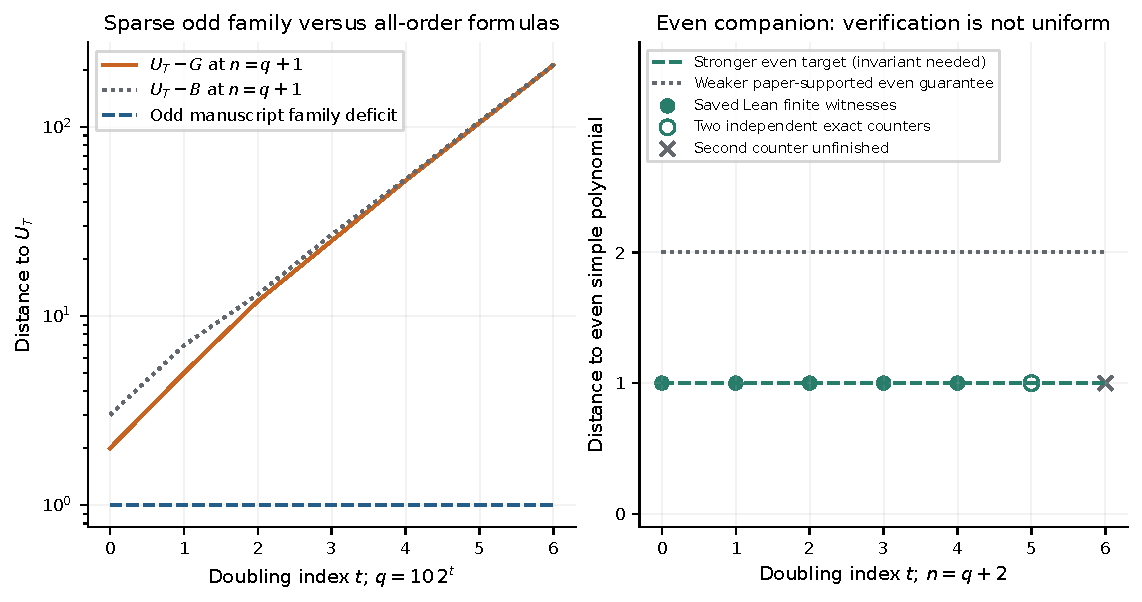
\includegraphics[width=0.88\linewidth]{figures/family-deficits.pdf}
\caption{The original sparse-family deficit plot, retained as a historical
numerical figure. Its arithmetic is unchanged. The family formulas now
have completed Lean existence proofs; any finite-check status encoded
in the original plot describes the September coordinate artifacts. The
new figure below compares the completed envelope.}
\label{fig:family-deficits}
\end{figure}

The independent adjacency and half-plane counters agree on the archived
321-, 322- and 641-line coordinate files, with $34132$, $34292$ and
$136532$ triangles. Their largest rational components have 916, 985 and
1103 decimal digits. The 642-line file passed adjacency and simplicity
checks but its separate direct recount was interrupted. That coordinate
artifact still has partial computational status. In contrast, existence
of some 642-line simple arrangement with at least $136852$ triangles is
now proved by Theorem~\ref{fam:even-conditional}. An existential proof
does not retrospectively certify the exact bytes of a saved coordinate
file.

\subsection{The first recursive envelope at every natural order}

Recall the previous retained bound $\Lbound(n)=\max\{G(n),C(n)\}$ in
\eqref{eq:envelope}. Define the sparse family contribution
\begin{equation}
 R(n)=\begin{cases}
 (q_t^2-4)/3,& n=q_t+1,\\
 (q_t^2-4)/3+q_t/2,& n=q_t+2,\\
 0,&\text{otherwise},
 \end{cases}
 \qquad q_t=10\cdot2^t,
 \label{fam:sparse-bound}
\end{equation}
and put
\begin{equation}
 H(n)=\max\{\Lbound(n),R(n)\}.
 \label{fam:new-envelope}
\end{equation}
The two cases have different parity and each determines $t$ uniquely.
The executable Lean definition uses the maximum of the candidates for
$0\le t\le n$, rather than an infinite search.

\begin{theorem}[Total retained and recursive envelope]\label{fam:all-n-envelope}
For every $n\in\N$, $\K(n)\ge H(n)\ge\Lbound(n)$. For every $t\ge5$,
\begin{align}
 H(q_t+1)-\Lbound(q_t+1)&=\floor{q_t/3}-2,\\
 H(q_t+2)-\Lbound(q_t+2)&=q_t/2-\floor{q_t/3}-2,
 \label{fam:exact-gains}
\end{align}
and both differences are positive.
\end{theorem}
\begin{proof}
Each nonzero candidate in \eqref{fam:sparse-bound} has a simple witness
by the preceding two theorems, hence an unrestricted witness. The
finite maximum chooses one such witness or a retained finite/baseline
witness; it is not an addition of incompatible triangle counts. If a
candidate occurs at order $n$, then $t<2^t\le n$, so the executable
finite maximum includes it. This is
\proofref{Kobon/RecursiveEnvelope.lean}{51}{\lean{all_n}}.

Since $q_t^2\equiv1\pmod3$ and $q_t$ is even, substitution in $G$ gives
\[
 T_t-G(q_t+1)=\floor{q_t/3}-2,\qquad
 T_t+q_t/2-G(q_t+2)=q_t/2-\floor{q_t/3}-2.
\]
All saved finite enhancements end at order 195. Thus
$\Lbound(n)=G(n)$ for $n>195$, as proved by
\lean{BBLFamilyBenchmarks.previous_envelope}. For $t\ge5$,
$q_t\ge320$ and both differences are positive. The formal strict-tail
statement is \lean{RecursiveEnvelope.strict_previous_tail}; uniqueness
of the sparse candidate identifies $H$ with that candidate here.
\end{proof}

At 321 and 322 lines the gains over the old verified envelope are
respectively 104 and 52; at 641 and 642 they are 211 and 105. The first
members do not displace stronger retained certificates: $21:133$,
$22:143$, $41:533$ and $42:553$ remain in $H$. All 138 coordinate
identities and their published attribution are retained. This theorem
improves the previous verified repository envelope at infinitely many
orders. It does not prove a numerical record against all published
families, and its off-family values retain the preceding all-order
linear deficit.

\begin{figure}[tb]
\centering
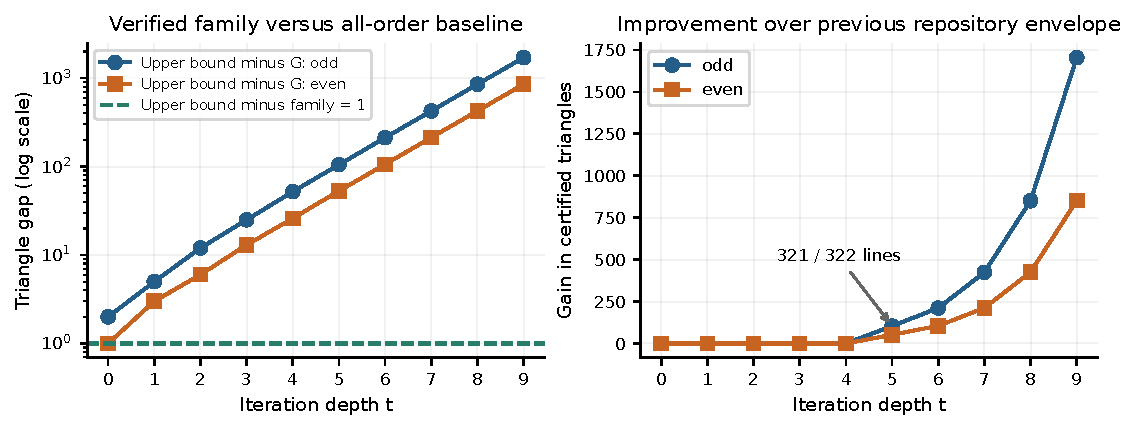
\includegraphics[width=0.95\linewidth]{figures/recursive-envelope.pdf}
\caption{The completed recursive family and the retained all-order bound.
The improvement is over the previous repository envelope; it is not a
numerical-priority comparison against all published constructions. The
upper comparisons refer to simple arrangements. Formula values are
proved in Lean; the plot is newly generated from those formulas.}
\label{fig:recursive-envelope}
\end{figure}

\subsection{Actual one-triangle optimality windows}

The October release also closes the geometric upper-bound bridge for
simple arrangements, as proved in Section~\ref{upper:simple-actual}.
This upgrades a comparison with a polynomial to a statement about the
actual extremal quantity.

\begin{corollary}[Simple optimality windows]\label{fam:optimality-windows}
For $q=10\cdot2^t$ and $t\ge0$, write $A=(q^2-4)/3$. Then
\begin{equation}
 A\le\Ks(q+1)\le A+1,\qquad
 A+q/2\le\Ks(q+2)\le A+q/2+1.
 \label{fam:windows}
\end{equation}
\end{corollary}
\begin{proof}
The lower halves are the constructed witnesses. For every simple
arrangement, the geometric upper results give
$3T\le n(n-2)$ and, for even $n\ge4$, $6T\le n(2n-5)$.
Substitution gives respectively
\[
 \floor{(q+1)(q-1)/3}=A+1,
 \qquad \floor{(q+2)(2q-1)/6}=A+q/2+1.
\]
The exact combined declarations are
\proofref{Kobon/BBLFamilyOptimality.lean}{29}{\lean{odd_window}} and
\proofref{Kobon/BBLFamilyOptimality.lean}{35}{\lean{even_window}}.
\end{proof}

The upper halves use standard logical axioms only; the lower halves
retain their seed's native dependencies. This one-triangle interval
need not be sharp at the smaller orders: the literature settles some
of them more precisely. In particular it is not an upper theorem for
arrangements with multiple concurrence, and it does not close the
unrestricted Kobon problem.

\subsection{Known optimal families and independent reproduction}

The classical dyadic five-line family must be kept separate from the
new compatible eleven-line realization.  A convenient normalized seed
uses intercepts $(-1,-\varepsilon,\varepsilon,1)$ and
\[
 x-v_jy=a_j,\qquad (v_0,v_1,v_2,v_3)=(-15,10,-10,30),
\]
together with $Y_0$.  The complete interval
$0<\varepsilon\leq10^{-5}$ has five certified triangles, all three
distinguished triangles, and two visible pairs.  Its central slopes
are $1/10$ and $-1/10$; the rightmost slope is $1/30$.
The normalization is deliberate: an earlier affine-equivalent numerical
realization had both central slopes negative, which was inadequate as
an unchecked premise for the sign convention in the published iterative
proof.  The corrected whole-parameter seed is verified in
\texttt{TamuraSeed5}.

The known optimal odd family and its simple even companions have
\begin{equation}
 q=4\cdot2^t,\qquad
 \Ks(q+1)\geq\frac{q^2-1}{3},\qquad
 \Ks(q+2)\geq\frac{q^2-1}{3}+\frac q2.
 \label{fam:tamura}
\end{equation}
The current finite certificates include
$5:5$, $6:7$, $9:21$, $10:25$, $17:85$, $18:93$, $33:341$,
$34:357$, $65:1365$, $66:1397$, $129:5461$, and $130:5525$.
These reproduce known numerical consequences of the affine family of
Forge and Ram\'irez Alfons\'in and BBL's odd-to-even discussion
\cite{forge1998,bbl2008}; they are not claimed as newly discovered
bounds. Theorem~\ref{fam:doubling} does not cover the small bases
$q=4,8,16$. The now completed uniform 33-line seed starts its formal
infinite tail at $q=32$, while retained finite certificates supply the
small cases.

Parpalak and Utkin supply a different straight-line family at
$q=18\cdot2^t$~\cite{parpalakutkin2026}.  Its odd count is
\begin{equation}
 \Ks(q+1)\geq\frac{q^2}{3}-1,
 \label{fam:pu}
\end{equation}
including $19:107$ and $37:431$.  The present work independently checked
their compatible 19-line seed on $0<\varepsilon\leq10^{-3}$ with 1632
exact endpoint determinant checks, a rational 107-triangle witness,
and all 17 distinguished triangles. The interval reproduction at 19
is separate from the now completed 37-line compatible tail below.
Both the seed and the family retain Parpalak--Utkin attribution.
The earlier BBL statement at $18\cdot2^t+1$ concerned pseudolines;
it cannot be used as a straight-line result without a realization
argument.  Applying Corollary~\ref{ext:odd-full} to the published
straight-line family gives the attributed simple even corollary
\[
 \Ks(q+2)\geq\frac{q^2}{3}+\frac q2-1,
\]
with $20:116$, $38:449$, $74:1763$, and $146:6983$.  Stronger nonsimple
published values at some of these orders concern $\K$, and do not
invalidate this simple-arrangement distinction.

\subsection{The closed integration interfaces and the Forge tail}

The verified 21-line base has the true tangent intercepts
\eqref{fam:old-grid} with $q=20$, fixed rational slopes, 132 triangles,
19 distinguished triangles, ten visible pairs, and the required
rightmost-line property for every $0<\varepsilon\le10^{-5}$.
Its finite interval checks use native evaluation; their analytic and
geometric soundness proofs are proved separately.

\begin{figure}[tb]
\centering
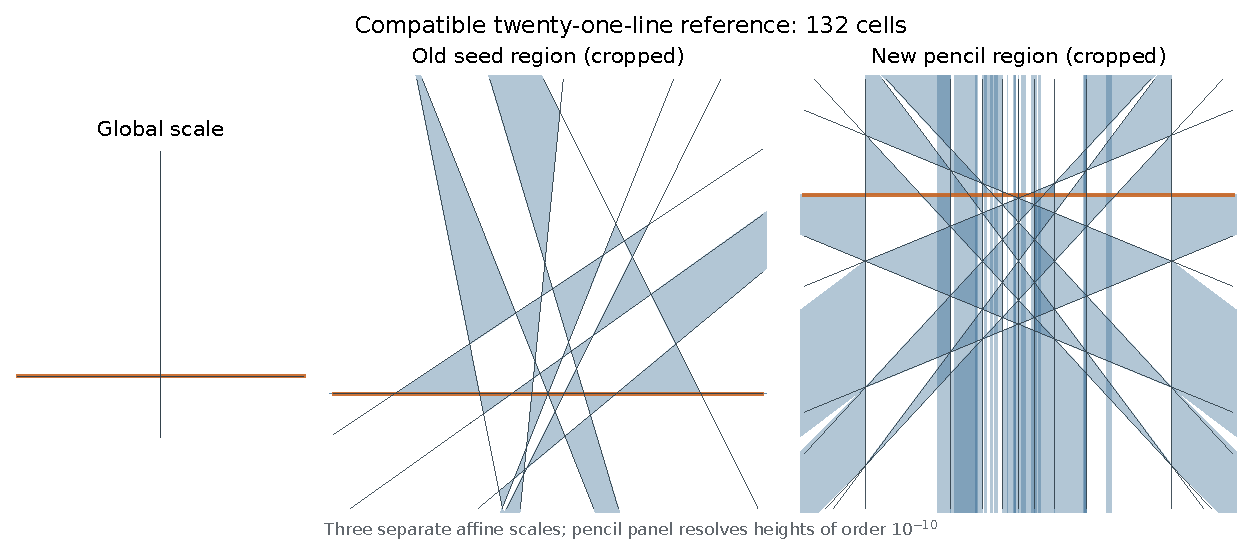
\includegraphics[width=0.88\linewidth]{figures/seed-21.pdf}
\caption{A 21-line hybrid checkpoint with 132 triangles. The global,
core and thin-pencil views illustrate scale separation. The finite
rendering is distinct from the true-tangent-grid parametric theorem in
\lean{BBLSeed21}. The normalized seed now starts the fully verified
recursion; the picture is not used as its proof.}
\label{fig:seed21}
\end{figure}

The September manuscript correctly identified four missing interfaces:
retained geometric data, whole-list transport under the next-grid
permutation, normalization of the 21-line grouped labels, and induction
on a positive parameter interval. All four are now complete. The
central source labels 5 and 6 have apex height $5\varepsilon/2$;
normalization preserves that actual point. The next central triangle
is retained independently of whether it appears in the counted list.
The invariant used in the successful induction is
\begin{equation}
 \exists\eta>0\quad\forall\varepsilon\in(0,\eta)\quad
 \exists\text{ a compatible counted seed at }(q,\varepsilon).
 \label{fam:recursive-quantifier}
\end{equation}
The former target
\begin{equation}
 q_t=20\cdot2^t,\qquad
 \Ks(q_t+1)\ge\frac{q_t^2-4}{3}
 \label{fam:21-target}
\end{equation}
is therefore a theorem, the tail of \eqref{fam:eleven-family}. The
visible-boundary interfaces are also closed by the same release.

The generic Forge--Ram\'irez Alfons\'in branch initially retained its
uniform seed premises. They are now discharged by the independent
\lean{OpenMathConstructionSeed33} modules. For every $t\ge0$,
\[
 \Ks(32\cdot2^t+1)\ge\frac{1024\cdot4^t-1}{3},\qquad
 \Ks(32\cdot2^t+2)\ge\frac{1024\cdot4^t-1}{3}+16\cdot2^t
\]
are actual simple real-line witnesses. The same rational reciprocal
slopes and finite statements preserved in the earlier stopped draft
are checked on $0<\varepsilon\le10^{-5}$. The sound Boolean certificate
engine completes the checks without changing their mathematical predicates.
\proofref{Kobon/OpenMathConstructionForgeFamily.lean}{25}{\lean{odd_family}}
and \proofref{Kobon/OpenMathConstructionForgeFamily.lean}{28}{\lean{even_family}}
instantiate the proved recursion; the same file proves both simple
optimality statements. These are formal completions of inherited
numerical formulas, not new construction records.

\subsection{A uniform 49-line compatibility certificate}
\label{fam:seed49}

The October search found a stronger compatible seed at order 49 using
fixed rational reciprocal slopes of denominator $10^{10}$. Its 48
intercepts are
\[
 -\tan\frac{23\pi}{48},\ldots,-\tan\frac\pi{48},
 -\varepsilon,\varepsilon,
 \tan\frac\pi{48},\ldots,\tan\frac{23\pi}{48}.
\]
Exact rational interval arithmetic verifies, throughout
$0<\varepsilon\le1/100$, a simple arrangement with 767 certified
triangles, all 47 distinguished-line caps and a positive central apex.
The fixed normal $(1,-2)$ has 24 visible pairs, including rightmost
pair $(0,48,49)$; the last slope is $1/3$ and the required boundary
inequalities hold uniformly. The full finite Lean base and its
normalization and visible-boundary bridges are now completed.

The analytic part is now inside Lean:
\sourcefile{Kobon/BBLTangent48Bounds.lean}{\lean{BBLTangent48Bounds}}
proves rational enclosures for each of the 23 positive tangent values,
using half-angle and reciprocal identities beginning with
$\tan(\pi/3)=\sqrt3$. The endpoint widths are at most
$5\cdot10^{-36}$. The exported finite predicates were independently
replayed: 1,176 direction checks, 18,424 simplicity checks, 37,583
triangle/support checks and 1,176 visibility/support checks passed.
Two independent exact cell counters also find 767 triangles at the
rational midpoint witness. The finite predicates and analytic-to-geometric
bridges now link the released data to the actual infinite theorem.

\begin{figure}[tb]
\centering
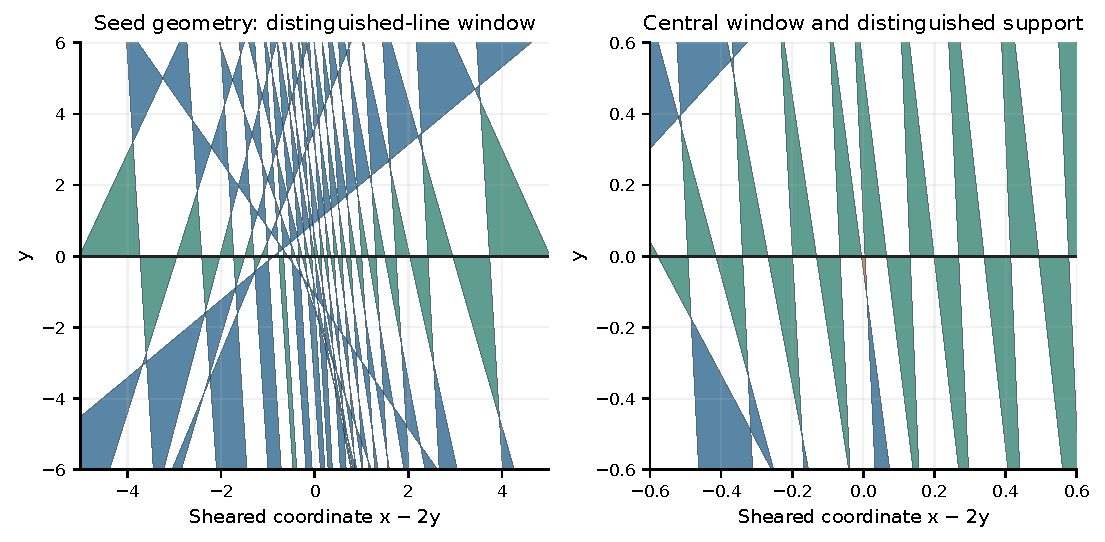
\includegraphics[width=0.98\linewidth]{figures/uniform49.pdf}
\caption{Two clipped windows of the rational midpoint witness for the
uniform 49-line seed, with $\varepsilon=1/200$. The invertible shear
$x'=x-2y$ makes the distinguished structure easier to see. The left
window has $x'\in[-5,5]$, $y\in[-6,6]$; the right has both coordinates
in $[-0.6,0.6]$. Ordinary certified cells are blue, distinguished caps
teal and the central cell orange. Distant cells lie outside these
windows: the panels do not display all 767 triangles. This finite view
illustrates the fully completed true-tangent uniform seed theorem.}
\label{fig:uniform49}
\end{figure}

The completed recursive instantiation gives
\begin{equation}
 q=48\cdot2^t,\qquad T_{\rm odd}=768\cdot4^t-1,
 \qquad T_{\rm even}=768\cdot4^t+24\cdot2^t-1
 \label{fam:49-conditional}
\end{equation}
at orders $q+1$ and $q+2$. The odd formula is exactly the tail $s=t+3$
of BBL's Theorem~1.3 for $n=6\cdot2^s+1$~\cite{bbl2008}; these are
not new numerical records. The contribution of this branch is an
explicit, well-conditioned uniform compatibility certificate and its
completed actual formal linkage. The declarations
\proofref{Kobon/BBL49VerifiedFamilies.lean}{36}{\lean{odd_family}} and
\proofref{Kobon/BBL49VerifiedFamilies.lean}{48}{\lean{even_family}}
have all seed hypotheses discharged. Combining these witnesses with the
classical simple upper bounds proves exactness in the simple model.
The known $50:792$ unrestricted witness is stronger than this orbit's
$50:791$ simple witness, so simple exactness is not unrestricted exactness.

Earlier positive-margin fits had moved triangles across infinity.
The successful fit additionally preserves the original affine sign
system. This illustrates why incidence or a projective order type alone
cannot certify the desired affine cell count.

A preceding search for a perfect compatible 21-line seed tested
11,547,910 floating proposals and 3,234 linear-feasibility programs
without improving 132. Those bounded failures were not impossibility
proofs. The exact obstruction in Section~\ref{exp:grid-obstruction}
now proves a much more precise limitation for a prescribed grid and
supplied classification; it still does not exclude other compatible
families or a different geometric construction.

\subsection{The compatible 37-line tail of the known 18-dyadic orbit}
\label{fam:seed37}

An independent refit of Poola's 37-line input retains 431 triangles and
35 distinguished-line caps on the actual tangent36 box
$0<\varepsilon\le10^{-8}$~\cite{poola2026}. The 17 positive tangent
enclosures are proved by analytic lemmas and rational kernel checks in
\lean{BBLTangent36Bounds}. The independent finite seed certificate and
normalization supply the complete input to the existing recursion.

\begin{theorem}[Completed 37-line orbit]\label{fam:37-complete}
For every $t\ge0$, put $q=36\cdot2^t$. Then
\begin{equation}
 \Ks(q+1)=432\cdot4^t-1,\qquad
 \Ks(q+2)=432\cdot4^t-1+18\cdot2^t.
 \label{fam:37-formula}
\end{equation}
\end{theorem}
\begin{proof}
The uniform compatible seed gives the first lower bound by closed
doubling. Its odd certified count has defect two. The completed
universal successor of Corollary~\ref{ext:odd-full} gives the second
lower bound at every depth, without an additional visible-pair finite
certificate. Substitution in the odd and even simple upper floors
gives matching upper bounds. These are
\proofref{Kobon/OpenMathConstructionFamily37.lean}{54}{\lean{odd_family}}
and \proofref{Kobon/OpenMathConstructionFamily37.lean}{58}{\lean{even_family}},
with simple exactness proved in the same module.
\end{proof}

Numerically this is the $q=18\cdot2^s$ straight-line series of
Parpalak--Utkin, starting at $s=t+1$, and its known even companions
\cite{parpalakutkin2026,parpalakutkinEven2026,blanc2011}.
The compatible exact certificate and formal linkage are the additions.
They raise the previous formal portfolio at $73,74$ from $1705,1752$
to $1727,1763$, and at $145,146$ from $6865,6960$ to $6911,6983$.
At 38 the retained unrestricted 450-cell witness remains stronger than
the simple optimum 449.

\subsection{A compatible 61-line seed and the visibility refinement}
\label{fam:seed61}

Poola's OpenMath submission supplies a 61-line point arrangement with
1190 triangles~\cite{poola2026}. Its original fixed slopes lose eight
cells as the two central tangent intercepts approach zero, so the point
count did not supply the uniform premise of the recursion. We refit
reciprocal slopes while preserving its affine orientation type, including
the chosen infinity support, at the limiting value $\varepsilon=0$.
A floating positive LP margin proposed the rational data; exact checks
then verified the whole true-tangent box $0<\varepsilon\le10^{-8}$.
The independent checker tests 35,990 simplicity conditions and 72,590
triangle/support conditions, retaining all 1190 triangles and all 59
axis caps. \lean{BBLTangent60Bounds} proves the actual 29 positive
tangent enclosures used by this box.

The first compatible refit has 28 visible pairs and normal
$(1,-20025598529/10^{10})$. A nonlocal feasible cap-cone ray mutation,
scored by the combined resource $T+V$, produces a second compatible
seed with 1190 triangles and \emph{29} visible pairs. Reflection and
shear restore the canonical rightmost boundary. Its fixed normal is
$(1,-8000441397/4000000000)$ and its central apex height is
$(20000000000/8777037)\varepsilon>0$. The sparse and original dense exact
checkers independently verify its triangle/cap box; every Lean finite
decision was replayed on the modified data. The original 28-pair seed
is retained separately.

\begin{theorem}[Actual 60-dyadic family]\label{fam:61-complete}
For every $t\ge0$, let $q=60\cdot2^t$. Then
\begin{align}
 \Ks(q+1)&\ge1200\cdot4^t-10,\label{fam:61-odd}\\
 \Ks(q+2)&\ge1200\cdot4^t+30\cdot2^t-11.\label{fam:61-even}
\end{align}
The counts are nine and ten below the corresponding simple upper floors.
\end{theorem}
\begin{proof}
The released uniform seed has $(r,T,V)=(15,1190,29)$ and supplies all
geometric and boundary premises of Theorems~\ref{fam:closed-iteration}
and~\ref{fam:visible-iteration}. Their recurrences give
\[
 T_t=1200\cdot4^t-10,\qquad V_t=30\cdot2^t-1.
\]
Exterior addition gives $T_t+V_t$. The simple upper floors at these
orders are $1200\cdot4^t-1$ and
$1200\cdot4^t+30\cdot2^t-1$, respectively. The actual declarations are
\proofref{Kobon/OpenMathConstructionParetoFamily61.lean}{48}{\lean{odd_family}}
and \proofref{Kobon/OpenMathConstructionParetoFamily61.lean}{51}{\lean{even_family}}.
The seed inherits seven explicit finite native Boolean roots; rescaling,
tangent analysis, normalization, boundary transport and iteration use
only standard logical axioms.
\end{proof}

The constant-gap calculation is a special case of the proved
\lean{BBLDeficitTransport}: the seed's odd triangle loss and visible-pair
loss are separately conserved by doubling. The allowable positive
parameter interval may shrink with depth. Neither a single fixed
positive $\varepsilon$ for all depths nor an optimum for the whole
60-dyadic class is asserted.

Relative to $G$, the gains are $20\cdot2^t-11$ in the odd branch and
$10\cdot2^t-11$ in the even branch. The odd examples are
$61:1190$, $121:4790$, $241:19190$, and $481:76790$.
The even examples are $62:1219$, $122:4849$, $242:19309$, and
$482:77029$. At 62 the retained $G(62)=1220$ is stronger.
The 29-pair improvement adds one triangle to the initial 28-pair even
formula at every depth; at $122,242,482$ this increases the newly
verified retained maxima from $4848,19308,77028$ to $4849,19309,77029$.

The finite 1190 count remains Poola's; doubling remains BBL's. A bounded
comparison of the BBL, Forge--Ram\'irez Alfons\'in, Parpalak--Utkin and
Savchuk sources did not locate this 60-dyadic straight-line orbit.
This supports treating the compatible orbit as a candidate new family,
but does not establish absolute numerical priority. No improved individual
Kobon optimum is inferred from this source search.

\begin{figure}[tb]
\centering
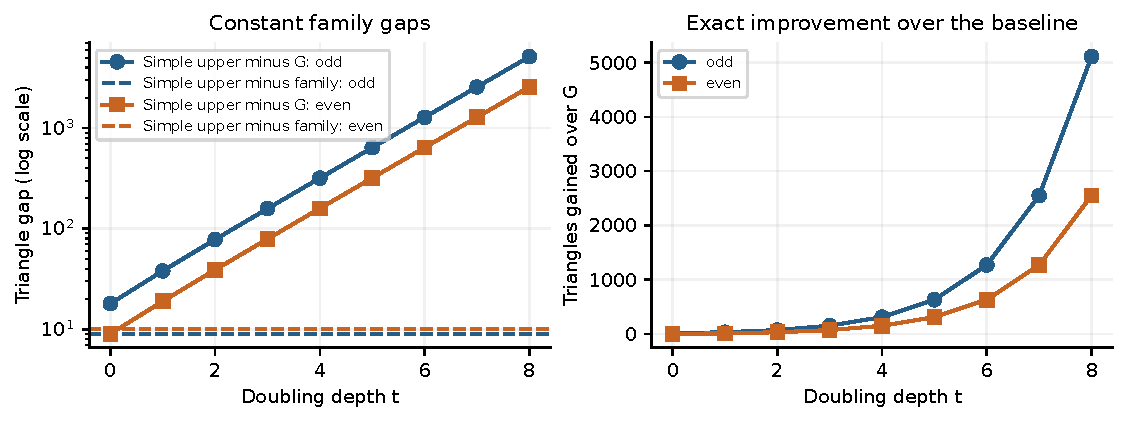
\includegraphics[width=0.95\linewidth]{new-family61-gaps.pdf}
\caption{Exact gaps of the 60-dyadic constructions to the classical simple
upper floors. The odd and strongest even gaps are constantly nine and
ten. The corresponding baseline gaps grow with the grid order. At depth
zero the baseline is stronger in the even case. These are formula
evaluations, with no fitted counts or unrestricted upper-bound claim.}
\label{fig:61-gaps}
\end{figure}

\subsection{The completed portfolio for every natural order}
\label{fam:portfolio-section}

\begin{table}[tb]
\centering\small
\begin{tabularx}{\linewidth}{@{}P{0.13\linewidth}P{0.25\linewidth}P{0.27\linewidth}X@{}}
\toprule
$q$ & Count at $q+1$ & Count at $q+2$ & Attribution and simple gaps\\
\midrule
$10\,2^t$ & $(100\,4^t-4)/3$ & Odd count $+5\,2^t$ & Eleven-derived; gaps $1,1$\\
$32\,2^t$ & $(1024\,4^t-1)/3$ & Odd count $+16\,2^t$ & Forge--Ram\'irez Alfons\'in; gaps $0,0$\\
$36\,2^t$ & $432\,4^t-1$ & Odd count $+18\,2^t$ & Parpalak--Utkin/Blanc tail; gaps $0,0$\\
$48\,2^t$ & $768\,4^t-1$ & Odd count $+24\,2^t$ & BBL tail; gaps $0,0$\\
$60\,2^t$ & $1200\,4^t-10$ & $1200\,4^t+30\,2^t-11$ & Compatible Poola refit; gaps $9,10$\\
\bottomrule
\end{tabularx}
\caption{Actual completed simple families for $t\ge0$. Gaps compare with
simple-model upper floors, not with the unrestricted maximum. The
numerical formulas of the middle three rows are inherited.}
\label{fam:orbit-table}
\end{table}

Let $F_a(n,t)$ equal the appropriate odd or even count in the row based
on $a\in\{32,36,48,60\}$, and zero away from those two orders. Define
\begin{equation}
 J(n)=\max\left\{H(n),\max_{0\le t\le n}
      \max_{a\in\{32,36,48,60\}}F_a(n,t)\right\}.
 \label{fam:portfolio-formula}
\end{equation}
\begin{theorem}[All-natural-order construction portfolio]\label{fam:portfolio}
For every $n\in\N$, there is an actual real-line arrangement with at
least $J(n)$ triangles. In particular $\K(n)\ge J(n)\ge H(n)$ and
$n^2\le3(J(n)+n)$.
\end{theorem}
\begin{proof}
Every nonzero candidate has an actual simple witness from the preceding
theorems. A zero candidate has the trivial lower witness. A finite maximum
selects one valid witness, and $t\le n$ includes every matching family
order. The prior envelope supplies an unrestricted witness if it is
stronger; no simplicity is then asserted for that chosen maximum.
This is \proofref{Kobon/OpenMathConstructionEnvelope.lean}{97}{\lean{all_n}},
with pointwise retention in
\proofref{Kobon/OpenMathConstructionEnvelope.lean}{100}{\lean{previous_le}}.
The quality inequality follows from the inherited all-order construction
and is proved at
\proofref{Kobon/OpenMathConstructionEnvelope.lean}{161}{\lean{quadratic_lower}}.
It does not improve the leading asymptotic coefficient.
\end{proof}

\begin{figure}[tb]
\centering
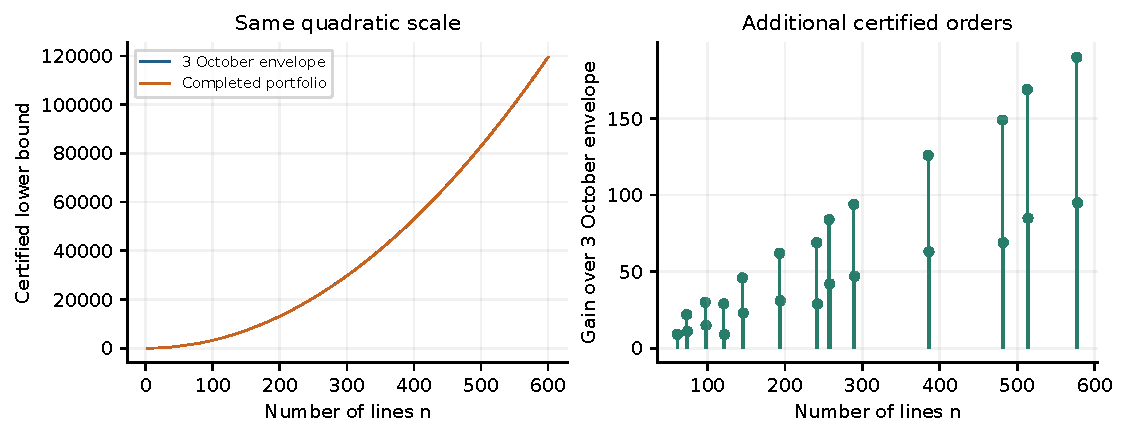
\includegraphics[width=0.95\linewidth]{new-family-orbits.pdf}
\caption{The completed family portfolio compared through exact formula
values. Uniform certification adds coverage of known optimal orbits;
the 60-dyadic orbit has the separate constant gaps in
Figure~\ref{fig:61-gaps}. Taking a maximum retains stronger finite
nonsimple witnesses. The figure makes no worldwide record comparison.}
\label{fig:family-orbits}
\end{figure}

\section{Multiplicity-sensitive upper-bound arguments}
\label{upper:scope}

This section develops upper estimates by separating ordinary crossings from finite multiple points. Actual elementary segments, incidence, clean-line charging and classical simple bounds were completed in the preceding release. The 5--6 October development additionally extracts cyclic fans, side matching, shared-core components and geometric escape from the real arrangement. The final structural theorems therefore have no supplied fan or aggregate budget premise. Their class restrictions and residual corrections remain explicit; they are not improved unrestricted numerical bounds for $\K$ depending only on the line count.

The distinction is necessary because the even-order estimates of Bartholdi--Blanc--Loisel and Blanc require simplicity~\citep{bbl2008,blanc2011}. The classical Cl\'ement--Bader envelope is treated as a reported external theorem~\citep{clementbader2007}; the local example in Section~\ref{upper:shared-fan} explains why we do not silently replace its proof by a bound on all shared edges incident to a multiple point.

\subsection{An exact elementary-segment identity}

\begin{definition}
For an arrangement of $n$ distinct affine lines, let $t_r$ be the number of finite intersection points incident to exactly $r$ lines, and let $P$ be the number of unordered parallel pairs. A bounded \emph{elementary segment} is the portion of an arrangement line between two consecutive finite intersection points. Let $E$ count these segments, $U$ count those incident to no triangular cell, and $D$ count those incident to two triangular cells. Let $a$ be the number of lines containing at least one finite intersection point, and put
\[
 S=\sum_{r\ge3}r(r-2)t_r,\qquad
 \delta=n(n-2)-3T,
\]
where $T$ is the number of bounded triangular cells.
\end{definition}

\begin{proposition}[Segment and defect identities]
\label{upper:identity}
For every such arrangement,
\begin{align}
 E&=n(n-1)-2P-S-a,\\
 3T&=E-U+D,\\
 \delta&=2P+S+a-n+U-D.
 \label{upper:defect-general}
\end{align}
If every line meets another line, then $a=n$ and $\delta=2P+S+U-D$.
\end{proposition}

\begin{proof}
Each nonparallel unordered pair contributes to exactly one finite point, so
\[
 n(n-1)-2P=\sum_{r\ge2}r(r-1)t_r.
\]
If a line has $s>0$ distinct finite intersection points, it contributes $s-1$ bounded elementary segments; an isolated line contributes none. Summing point-line incidences gives
\[
 E=\sum_{r\ge2}r t_r-a.
\]
Subtracting these expressions yields the first identity. Each triangular cell uses three elementary segments. A segment is incident to zero, one, or two such cells, so the total number of triangle-side incidences is $E-U+D$. Substitution into the definition of $\delta$ gives the last identity.
\end{proof}

The term $D$ cannot be dropped in a nonsimple arrangement. Multiple points reduce the available segment count by $S$, but sharing can compensate for some of that loss. This is precisely the interaction that a classical upper proof must control.

\begin{lemma}[A shared side has a multiple endpoint]
\label{upper:shared-endpoint}
An elementary segment incident to two bounded triangular cells cannot have both endpoints ordinary, where an ordinary point is incident to exactly two arrangement lines.
\end{lemma}

\begin{proof}
At each ordinary endpoint there is a unique supporting line other than the line containing the segment. Both adjacent triangles would therefore have the same three supporting lines. Three distinct lines have at most one bounded triangular region, whereas the two incident cells lie on opposite sides of the shared segment. This is impossible.
\end{proof}

The parity estimates below assume even $n\ge4$ and pairwise nonparallel lines. The later component statements hold for either parity at $n\ge2$. Let the \emph{core} consist of the finite points of multiplicity at least three. Write
\[
 q=\sum_{r\ge3}t_r,\qquad I=\sum_{r\ge3}r t_r,
\]
and let $h$ count the lines meeting the core. Let $D_1$ count shared elementary segments with exactly one core endpoint and $D_2$ those with two core endpoints. By Lemma~\ref{upper:shared-endpoint}, $D=D_1+D_2$, and hence
\begin{equation}
 \delta=S+U-D_1-D_2.
 \label{upper:core-identity}
\end{equation}

\subsection{Parity on a line outside the core}

A line is \emph{clean} if it contains no core point. The following argument adapts the local parity method in Blanc's Section~2~\citep{blanc2011}. Its proof is included because the transverse lines may have multiple intersections away from the clean line.

\begin{lemma}[Clean-line charging]
\label{upper:clean-charge}
For even $n\ge4$ and pairwise nonparallel lines,
\begin{equation}
 n-h\le2U+D_1.
 \label{upper:charging}
\end{equation}
\end{lemma}

\begin{proof}
First fix a clean line $L$, place it horizontally, and number its $n-1$ crossings from left to right. Let $R_i$ be the transverse line at crossing $i$. Denote the bounded segment of $L$ between crossings $i$ and $i+1$ by $\ell_i$, and its two exterior rays by $\ell_0$ and $\ell_{n-1}$. Write $p_i^+$ and $p_i^-$ for the faces above and below $\ell_i$, and $r_i^+,r_i^-$ for the elementary transverse pieces of $R_i$ immediately above and below $L$. A transverse piece may be a bounded segment or an unbounded ray.

We show that some bounded $r_i^{\pm}$ is unused or shared. Suppose otherwise: every bounded transverse piece is incident to exactly one triangle. Each bounded $\ell_i$ is unshared by Lemma~\ref{upper:shared-endpoint}.

If both $p_1^+$ and $p_1^-$ are nontriangular, then $r_1^+$ and $r_1^-$ are unused: their other adjacent faces meet the exterior ray $\ell_0$. At least one of these transverse pieces is bounded, because $R_1$ meets another transverse line. This contradicts the supposition. Reflecting across $L$ if necessary, assume $p_1^+$ is triangular; $p_1^-$ is then not.

For $1\le i\le n-2$, prove the following assertions together:
\begin{enumerate}[label=(\roman*)]
\item if $i$ is even, $p_i^+$ is nontriangular; if $i$ is odd, $p_i^-$ is nontriangular;
\item if both faces at $\ell_{i-1}$ are nontriangular, then $p_i^-$ is triangular for even $i$, and $p_i^+$ is triangular for odd $i$.
\end{enumerate}
The base case follows from the choice of $p_1^+$ and the unbounded faces at $\ell_0$. Consider an even step; the odd step exchanges signs. If $p_{i-1}^+$ is triangular, then $p_i^+$ cannot be triangular, since otherwise the two triangles share the bounded piece $r_i^+$, contrary to the supposition. Assertion (ii) has a false antecedent in this case.

Otherwise both $p_{i-1}^+$ and $p_{i-1}^-$ are nontriangular by the preceding odd step. This cannot happen for $i=2$, so $i\ge4$. The earlier even step makes $p_{i-2}^+$ nontriangular. Hence $r_{i-1}^+$ is unused, and must be unbounded. The intersection of $R_{i-1}$ and $R_i$ must consequently lie below $L$. It follows that $r_i^-$ is bounded. Its left adjacent face is nontriangular, so its right adjacent face $p_i^-$ must be triangular. Since $\ell_i$ is unshared, $p_i^+$ is nontriangular. This proves both assertions.

Now $n-2$ is even, so $p_{n-2}^+$ is nontriangular. If $p_{n-2}^-$ is also nontriangular, both pieces at the last crossing are unused and at least one is bounded, again a contradiction. Otherwise $p_1^+$ and $p_{n-2}^-$ are triangular, while $r_1^-$ and $r_{n-1}^+$ are unused. The lines $R_1$ and $R_{n-1}$ intersect. If their intersection is below $L$, then $r_1^-$ is bounded; if above, then $r_{n-1}^+$ is bounded. This is the final contradiction.

Charge each clean line to one bounded unused or shared transverse segment supplied by this argument. An unused segment can receive at most two charges, one at each ordinary endpoint. A shared segment must have a multiple endpoint, so it can receive at most one charge if counted by $D_1$, and none if counted by $D_2$. There are $n-h$ clean lines, giving~\eqref{upper:charging}.
\end{proof}

\begin{remark}[Why parallel pairs have been excluded]
Three parallel vertical lines and one horizontal line give a clean horizontal line whose transverse pieces are all unbounded. Thus simply removing parallel-participating lines from the set to be charged does not prove the lemma. The identities of Proposition~\ref{upper:identity} allow parallels, but the charging argument above does not. Every subsequent upper estimate in this section retains the pairwise nonparallel hypothesis.
\end{remark}

Combining~\eqref{upper:core-identity} and~\eqref{upper:charging} gives the basic budget
\begin{equation}
 2\delta\ge n+2S-h-3D_1-2D_2.
 \label{upper:basic-budget}
\end{equation}
The remaining problem is to bound the shared-side contribution at the core.

\subsection{The geometric obstruction in a cyclic fan}

At an $r$-fold point $v$, the incident lines determine $2r$ rays in cyclic order, with opposite rays separated by $r$ positions. Let $d_1(v)$ count shared elementary segments starting at $v$ and ending at an ordinary point, and let $d_2(v)$ count those ending at another core point. A ray supports at most one such incident elementary segment.

\begin{lemma}[No long run of ordinary-ended shared rays]
\label{upper:no-long-run}
For $r\ge3$, no $r-1$ consecutive rays at an $r$-fold point can all support segments counted by $d_1(v)$.
\end{lemma}

\begin{proof}
Such a run would border $r$ consecutive triangular sectors. At the ordinary endpoint of each selected shared segment, the opposite supporting lines of the two neighboring triangles must coincide: besides the radial line through $v$, only one arrangement line passes through that endpoint. Propagating this equality makes the opposite sides of all $r$ triangles lie on one line $M$.

The line $M$ would meet $r+1$ consecutive rays from $v$, which include an opposite pair. A line meeting both open opposite rays must contain their connecting segment and hence $v$. But the opposite side of a nondegenerate triangle with vertex $v$ cannot lie on a line through $v$. This contradiction proves the lemma.
\end{proof}

This is an actual geometric statement, not an assumed combinatorial prohibition. The Lean module \texttt{FanGeometry} proves uniqueness and propagation of opposite supports for real lines and points. The module \texttt{CyclicFan} supplies the cyclic-to-geometric bridge from triangular sectors, antipodal rays and ordinary selected endpoints.

\begin{proposition}[Local fan budget]
\label{upper:fan-budget}
At every finite point of multiplicity $r\ge3$,
\begin{equation}
 d_1(v)\le2r-3,\qquad 3d_1(v)+d_2(v)\le6r-6.
 \label{upper:local-fan-budget}
\end{equation}
\end{proposition}

\begin{proof}
Count selected rays in all $2r$ cyclic windows of length $r-1$. Each window contains at most $r-2$ selected rays by Lemma~\ref{upper:no-long-run}, and each selected ray belongs to exactly $r-1$ windows. Therefore
\[
 (r-1)d_1(v)\le2r(r-2).
\]
If $d_1(v)\ge2r-2$, the left side is at least $2(r-1)^2=2r(r-2)+2$, a contradiction. Finally $d_1(v)+d_2(v)\le2r$, so
\[
 3d_1(v)+d_2(v)=2d_1(v)+(d_1(v)+d_2(v))\le6r-6.
\]
\end{proof}

The cyclic double count is proved in \texttt{FanCount}. The theorem \lean{CyclicFan.selected_card_le} combines it with the real geometric obstruction, without assuming the no-long-run conclusion as an unexplained premise.

\subsection{A weighted bound for an arbitrary finite core}

\begin{proposition}[Multiplicity-weighted defect estimate]
\label{upper:weighted}
Let $n\ge4$ be even and let the arrangement be pairwise nonparallel. Then
\begin{equation}
 2\delta\ge n+\sum_{r\ge3}(2r^2-11r+6)t_r.
 \label{upper:weighted-defect}
\end{equation}
\end{proposition}

\begin{proof}
Each $D_1$ segment has exactly one core endpoint and each $D_2$ segment has two. Summing~\eqref{upper:local-fan-budget} gives
\[
 3D_1+2D_2\le6I-6q.
\]
Also $h\le I$, since every core line contributes at least one point-line incidence. Inserting both inequalities into~\eqref{upper:basic-budget} yields
\[
 2\delta\ge n+2S-7I+6q,
\]
which is~\eqref{upper:weighted-defect} after expanding $S,I,q$.
\end{proof}

The local weights are $-9,-6,1,12,27$ at multiplicities $3,4,5,6,7$, respectively. Consequently the obstruction to recovering a simple-style parity defect is concentrated at triple and quadruple points; higher multiplicity has a positive weight in this accounting.

\begin{corollary}[Nonnegative core weight]
\label{upper:high-multiplicity}
Under the hypotheses of Proposition~\ref{upper:weighted}, if
\[
 \sum_{r\ge3}(2r^2-11r+6)t_r\ge0,
\]
then
\[
 T\le\left\lfloor\frac{n(n-5/2)}3\right\rfloor.
\]
In particular, this holds if every finite multiple point has multiplicity at least five.
\end{corollary}

\begin{proof}
The weighted estimate implies $\delta\ge n/2$, giving the displayed upper bound by the definition of $\delta$. For $r\ge5$, the exact factorization
\[
 2r^2-11r+6=1+(r-5)(2r-1)\ge1
\]
proves the stated sufficient condition.
\end{proof}

This extends the same polynomial to a restricted nonsimple class. It says nothing comparable for a general core consisting of many triple points. Numerical first priority for this restricted consequence has not been established.

\subsection{A sharper estimate with at most two core points}

\begin{lemma}[A fan with at most one core-to-core ray]
\label{upper:one-core-ray}
If $d_2(v)\le1$ at a point of multiplicity $r\ge3$, then $d_1(v)\le2r-4$.
\end{lemma}

\begin{proof}
Mark which of the $2r$ sectors at $v$ are triangular. A ray supports a shared elementary segment exactly when both neighboring sectors are triangular. If every sector is triangular, every ray is shared; deleting at most one $d_2$ ray leaves a run of at least $2r-1$ selected rays, contradicting Lemma~\ref{upper:no-long-run}. Hence a nontriangular sector exists.

Suppose $d_1(v)\ge2r-3$. Two separated nontriangular sectors exclude at least four shared rays, as do three consecutive nontriangular sectors. Both situations are impossible. If exactly one sector is nontriangular, the shared rays form a path of length $2r-2$. Deleting at most one $d_2$ ray leaves at most two selected runs. Their total capacity is $2(r-2)$, less than the required $2r-3$. If exactly two adjacent sectors are nontriangular, at most $2r-3$ shared rays remain. All would have to be selected, forming a run of length $2r-3>r-2$. These cases exhaust the possibilities and prove the lemma.
\end{proof}

\begin{theorem}[At most two finite multiple points]
\label{upper:two-core}
An arrangement of an even number $n\ge4$ of pairwise nonparallel affine lines with at most two finite multiple points satisfies
\begin{equation}
 T\le\left\lfloor\frac{n(n-5/2)}3\right\rfloor+1.
 \label{upper:two-core-upper}
\end{equation}
More precisely, the defect bounds are $\delta\ge n/2$ if $q=0$, $\delta\ge n/2-1$ if $q=1$, and $\delta\ge n/2-3$ if $q\le2$.
\end{theorem}

\begin{proof}
With at most two core points, at most one ray at a core point can terminate at another core point. Lemma~\ref{upper:one-core-ray} gives $D_1\le2I-4q$. There is at most one core-to-core shared segment, so $D_2\le q(q-1)/2\le1$. Moreover,
\[
 h\le I-D_2,
\]
because any such segment lies on a line counted twice in the core-incidence total and once among the core lines. Substitution in~\eqref{upper:basic-budget} yields
\[
 2\delta\ge n+\sum_{r\ge3}(2r^2-11r+12)t_r-D_2.
\]
For $r\ge3$,
\[
 2r^2-11r+12=-3+(r-3)(2r-5)\ge-3.
\]
Thus $2\delta\ge n-3q-D_2\ge n-7$. Since $n$ and $2\delta$ are even, $2\delta\ge n-6$. Rearranging gives~\eqref{upper:two-core-upper}. If $q=1$, then $D_2=0$ and the inequality $2\delta\ge n-3$ rounds to $2\delta\ge n-2$; if $q=0$, it gives $2\delta\ge n$ directly.
\end{proof}

The hypotheses are attained by externally attributed exact constructions. Table~\ref{upper:restricted-attainment} records examples whose pairwise nonparallel status, triangle count, and two triple points were checked exactly. Their equality with~\eqref{upper:two-core-upper} proves sharpness within this restricted class, not optimality over all classical arrangements.

\begin{table}[htbp]
\centering\small
\begin{tabular}{@{}rrrl@{}}
\toprule
$n$ & $T$ & Restricted upper & Coordinate provenance\\
\midrule
8 & 15 & 15 & Earlier construction, retained in the current gallery\\
14 & 54 & 54 & Maiorana, two-triple-point witnesses\\
26 & 204 & 204 & Parpalak--Utkin gallery\\
50 & 792 & 792 & Parpalak--Utkin gallery\\
\bottomrule
\end{tabular}
\caption{Attainment in the class covered by Theorem~\ref{upper:two-core}. Sources: \citet{maiorana2026,parpalakutkinGallery2026}. These are not new numerical records claimed by this paper.}
\label{upper:restricted-attainment}
\end{table}

ProofAtlas reports a stronger restriction-specific result at $n=14$, covering up to four finite multiple points~\citep{proofatlas2026}. Its proof was not independently reproduced here. Our two-point estimate covers all even orders and arbitrary core multiplicities, but neither that fact nor the table establishes priority for the restricted theorem.

\subsection{A checked shared-fan example and the limits of smoothing}
\label{upper:shared-fan}

Consider the six lines
\begin{equation}
 x=0,\quad y=0,\quad x+y=3,\quad x-y=0,\quad
 2x+y=3,\quad x+2y=3.
 \label{upper:median-lines}
\end{equation}
They are the three sides of a triangle and its three medians. There are six bounded triangular cells and four triple points. At $v=(1,1)$, six distinct nonzero elementary radial segments are shared sides, each belonging to two of those cells. Three have ordinary other endpoints and three have multiple other endpoints, giving $d_1(v)=d_2(v)=3$; globally $D_1=D_2=3$.

\begin{figure}[htbp]
\centering
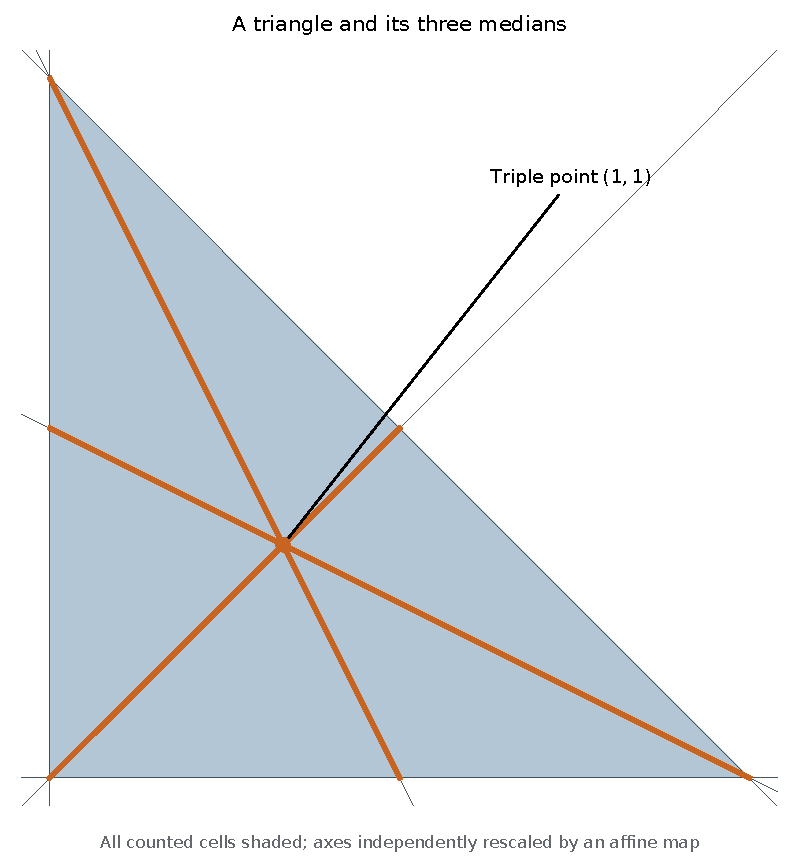
\includegraphics[width=0.75\textwidth]{figures/shared-fan.pdf}
\caption{The exact arrangement~\eqref{upper:median-lines}. Six triangular cells meet around the central triple point, and all six radial sides are shared. This refutes only a literal local incidence reading of the shared-pair statement in Cl\'ement--Bader's Lemma~1; it does not refute their final upper theorem. The figure is newly generated from the integer equations.}
\label{fig:shared-fan}
\end{figure}

The \texttt{SharedFan} module proves the real geometric facts: each designated triangle has nonempty uncut interior, the six interiors are pairwise disjoint, the radial segments are distinct and elementary, and each is a side of two distinct triangles. The proof uses ordinary kernel checking.

This matters when interpreting the Cl\'ement--Bader proof. Its local shared-pair sentence cannot literally bound all shared segments incident to a multiple point by two. An intended assignment of each shared side to one endpoint would be a different assertion requiring global justification. The example has only six triangles, below the reported seven-triangle upper bound at order six; it is therefore not a counterexample to that upper theorem. The present paper leaves that distinction explicit and uses the separate $D_1,D_2$ accounting instead.

Nor can one justify a simple upper bound merely by perturbing every multiple point. For a retained two-triple-point Maiorana $14{:}54$ witness, the four local generic resolution types have triangle counts $52,52,53,52$. These counts were checked with exact arithmetic; they are finite experimental evidence, not a new Lean theorem classifying all perturbations. They demonstrate why a universally nondecreasing smoothing argument needs more than the existence of a small generic perturbation. Our global upper argument never assumes such monotonicity.

\subsection{Actual arrangement extraction and simple upper theorems}
\label{upper:simple-actual}

The formal inventory is now built from an actual finite injective family
of certified triangles in $n\ge2$ pairwise nonparallel lines. It may
be a proper subset of all triangular cells. The quantities $U,D_1,D_2$
are defined relative to this selected family. The cell theorem proves
interior disjointness, and the side-emptiness theorem proves that each
side has consecutive endpoints on its supporting line.

An unordered endpoint pair represents one geometric side. At most two
pairwise interior-disjoint nondegenerate triangles can share that side:
three would put two on the same side of its support, forcing their
interiors to overlap near an interior base point. Counting triangle-side
incidences therefore gives $3T=E-U+D_1+D_2$. Pair counting proves
$\sum r(r-1)t_r=n(n-1)$ and the actual consecutive-edge inventory gives
$E=n(n-2)-S$. Thus
\begin{equation}
 \delta=S+U-D_1-D_2
 \label{upper:actual-identity}
\end{equation}
is proved from geometry by
\sourcefile{Kobon/UpperEdgeInventory.lean}{\lean{certificate_defect_identity}};
capacity, incidence and edge cardinality are conclusions of the proof,
not assumed numerical identities.

\begin{theorem}[Actual clean-line charging and simple bounds]
\label{upper:actual-simple}
Let $n\ge4$ be even. For any pairwise nonparallel real arrangement and
finite injective certified triangle family,
\begin{equation}
 n-h\le2U+D_1.
 \label{upper:actual-charging}
\end{equation}
For every simple arrangement with $T$ certified triangular cells,
\begin{equation}
 3T\le n(n-2)\quad(n\ge2),\qquad
 6T\le n(2n-5)\quad(n\ge4\text{ even}).
 \label{upper:actual-simple-bounds}
\end{equation}
\end{theorem}

\begin{proof}
The parity proof of Lemma~\ref{upper:clean-charge} can also be organized
as an odd-cardinality matching contradiction, which is the formal route.
A clean line has exactly $n-1$ distinct crossings. One common open
half-plane contains a further crossing on every transverse support.
Choose in that half-plane the consecutive bounded segment incident to
each clean-line crossing. Existence is obtained from the nearest actual
intersection, with the bounded-side and uniqueness lemmas handling
both signs.

If every chosen edge had degree one in the certified triangle family,
its unique triangle would have its base on the clean line: at an ordinary
crossing a triangle must use one of the two incident supports. Consecutive
edge uniqueness and interior disjointness then make these bases a
disjoint two-element cover of the clean-line crossings. Such a cover
has even cardinality, contradicting $n-1$ odd. Hence some incident
bounded edge has degree zero or two. A degree-two edge has a multiple
other endpoint by the shared-side lemma, so it is counted by $D_1$.

Choose one resulting charge for each clean line. A fixed ordinary
endpoint of an edge determines at most one clean transverse line.
An unused edge has at most two such endpoints and receives at most two
charges; a $D_1$ edge has exactly one ordinary endpoint and receives
at most one. This proves \eqref{upper:actual-charging}. The extraction,
choice and fiber bounds are all in
\proofref{Kobon/UpperCleanCharging.lean}{100}{\lean{certificate_clean_line_budget}},
using \lean{UpperCleanHalfplane}, \lean{UpperCleanEdges},
\lean{UpperCleanPairing} and \lean{UpperCleanCover}. No charge-existence
or pairing premise remains.

For a simple arrangement the core is empty, so $S=D_1=D_2=h=0$.
Equation~\eqref{upper:actual-identity} gives $3T=n(n-2)-U$, proving the
first bound. In the even case $n\le2U$, so
$6T=2n(n-2)-2U\le n(2n-5)$.
The \lean{SimpleLowerBound} versions extract the injective finite family
from its duplicate-free triangle list. These are
\sourcefile{Kobon/UpperSimpleOptimality.lean}{\lean{simple_lower_bound_upper}}
and
\sourcefile{Kobon/UpperEvenSimpleOptimality.lean}{\lean{simple_lower_bound_even_upper}}.
\end{proof}

The integer floor forms follow immediately. These classical inequalities
retain their earlier attribution, including Blanc's even parity bound.
Their contribution here is a complete real-geometric formalization with
standard logical axioms only. In particular, the retained simple
$44:608$ certificate attains $\lfloor44(88-5)/6\rfloor=608$; this
proves simple optimality at that order, not unrestricted optimality.
Theorem~\ref{upper:actual-simple} does not justify applying the even
polynomial to nonsimple witnesses such as $14:54$.

\subsection{Extremal fans and strengthened local restrictions}
\label{upper:extremal-fans}

\begin{theorem}[Equality structure of a supplied cyclic fan]
\label{upper:extremal-structure}
Consider actual local sector data at an $r$-fold point, $r\ge3$, satisfying
the cyclic order, antipodality, triangle and ordinary-endpoint conditions
of \lean{UpperFan.Sectors}. If $d_1=2r-3$, every sector is triangular
and $d_2=3$. Consequently,
\begin{equation}
 d_2\le2\Longrightarrow d_1\le2r-4,
 \qquad 3d_1+d_2\le6r-8+2e,
 \label{upper:extremal-weight}
\end{equation}
where $e=1$ when $d_1=2r-3$ and $e=0$ otherwise.
\end{theorem}

\begin{proof}
The no-long-run property from Lemma~\ref{upper:no-long-run} holds for
the selected ordinary-ended shared rays. If a sector were missing,
both bounding rays would be absent from that selected set. The cyclic
window count with these adjacent omissions strengthens its cardinality
bound to $2r-4$. Thus the extremal case has every sector present; all
$2r$ rays are then shared. Subtracting $d_1=2r-3$ gives $d_2=3$.
If $d_2\le2$, equality in the old bound is therefore impossible.
In the nonextremal case,
$3d_1+d_2=2d_1+(d_1+d_2)\le2(2r-4)+2r$; in the extremal case its
value is $6r-6$. These give \eqref{upper:extremal-weight}.
The exact proofs are
\proofref{Kobon/UpperFan.lean}{171}{\lean{all_sectors_of_extremal}},
\proofref{Kobon/UpperFan.lean}{187}{\lean{core_shared_card_eq_three_of_extremal}}
and \proofref{Kobon/UpperFan.lean}{227}{\lean{weighted_local_bound}}.
\end{proof}

This strengthens the previous manuscript's local hypothesis $d_2\le1$
to $d_2\le2$. The formerly supplied local interface is now extracted
from every actual core, as described below. A supported extreme core
cannot carry the full extremal fan
when its core-ended rays are identified with points in the supporting
closed half-plane (\lean{UpperFanSupport} and
\lean{UpperCoreBoundary}). Also, two full extremal triple fans cannot
be adjacent across the same matched elementary side with its two
neighboring certified triangles (\lean{UpperTripleFan}). The latter
uses the actual coincident endpoints and opposing adjacent sectors;
an arbitrary pair of abstract fan records need not supply that matching.
The completed arrangement wrapper derives it from the original selected
triangle occurrences, rather than assuming compatible abstract records.

\subsection{Actual fan extraction, matching and global assembly}
\label{upper:actual-global}

At each core the development orders the actual supporting directions by
an admissible affine chart, appends their opposite representatives, and
obtains a cyclic list of $2r$ nonzero rays. Consecutive selected triangle
sectors determine actual side endpoints. Simplicity of the elementary
segment inventory identifies a shared ray with its unique ordinary or
core endpoint, and injectivity of the selected triangle labels identifies
its two neighboring cell occurrences. Thus the local ordinary and core
ray counts equal $d_1(v)$ and $d_2(v)$, rather than supplied numerical
surrogates. The actual local bound is
\proofref{Kobon/UpperOpenMathActualFans.lean}{197}{\lean{certificate_local_fan_bound}};
matching along a shared elementary edge is
\proofref{Kobon/UpperOpenMathActualMatching.lean}{22}{\lean{certificate_neighbor_matching}}.
The geometric no-long-run and extremal conclusions above now apply to
these extracted records at every core.

Double counting their actual side incidences gives
$\sum_vd_1(v)=D_1$ and $\sum_vd_2(v)=2D_2$. In particular, the
weighted sum and exceptional-fan corrections no longer require a global
fan premise. The result is assembled in
\proofref{Kobon/UpperOpenMathGlobalFans.lean}{78}{\lean{certificate_weighted_fan_sum}}
and \proofref{Kobon/UpperOpenMathGlobalFans.lean}{204}{\lean{certificate_defect_even}}.
This completes the formal geometric scope of
Proposition~\ref{upper:weighted} and its higher-multiplicity corollary.
The previously conditional refined budget is now an actual theorem:
\begin{equation}
 2\delta\ge n+2S-7I+8q-2e+D_2,
 \label{upper:refined-conditional}
\end{equation}
where $e$ counts full extremal fans with ordinary degree $2r-3$.
The stronger boundary-sensitive assembly proves the two-core theorem
and the three-core estimate with their actual geometry, in
\proofref{Kobon/UpperOpenMathBoundaryBudgets.lean}{128}{\lean{certificate_three_core_upper}}
and \proofref{Kobon/UpperOpenMathBoundaryBudgets.lean}{137}{\lean{certificate_two_core_upper}}.
The former gives, when $q\le3$ and $n=2m$,
\begin{equation}
 \delta\ge m-6,\qquad T\le\floor{m(4m-5)/3}+2,
 \label{upper:three-core-conditional}
\end{equation}
equivalently $6T\le n(2n-5)+12$. The retained labels record the historical
conditional statements; their arrangement extraction is now complete.
For $q\le1$, or $q\le2$ with at most one triple core, the sharper
rounding is $6T\le n(2n-5)+2$, proved by
\sourcefile{Kobon/UpperOpenMathSparseUpper.lean}{\lean{UpperOpenMathSparseUpper}}.
These are restricted numerical consequences at every even order.

Several independent exact resources retain geometry that earlier budgets
discarded. Let $C$ count core endpoints of bounded nonshared elementary
sides, and $R_c$ count unbounded rays at cores. Actual first/last vertex
flags give
\begin{align}
 D_1+2D_2+C+R_c&=2I,\\
 2\delta&=2\sum_{r\ge3}r(r-3)t_r+2U+C+R_c-D_1.
 \label{upper:ray-identities}
\end{align}
The source \lean{UpperOpenMathRayResources} proves both identities.
The actual shared-core graph has core vertices and $D_2$ edges, including
isolated vertices in its component partition. Its component hull points
consume at least two nonshared or ray resources each. If $b_h$ is the
sum of the numbers of supporting hull points of the individual components,
then the completed hull estimate is
\begin{equation}
 2\delta\ge2U+2\sum_{r\ge3}r(r-4)t_r+3q+3b_h.
 \label{upper:component-hull}
\end{equation}
It follows from separately bounding ordinary sharing and total sharing
at each supported core; see
\proofref{Kobon/UpperOpenMathComponentHullDeficit.lean}{86}{\lean{certificate_component_hull_deficit}}.
If all core multiplicities are at least $R\ge4$, this gives
$6T+(2R(R-4)+3)q+3b_h+2U\le2n(n-2)$.
The cases $R=4,5$ retain penalties $3q,13q$, respectively.
These are structural estimates, not a formula for the unrestricted maximum.

\subsection{Degree-free structural bounds and their local counts}
\label{upper:degree-free}

All statements in this subsection concern $n\ge2$ pairwise nonparallel
real lines and an arbitrary finite injective family of certified triangular
cells. All core, side and component counts are extracted from that family.
At a core put $a=d_1$, $d=d_2$. A \emph{marked port} is a shared core ray
whose two neighboring shared rays end at ordinary vertices. Let $m$ be
the number of such ports. In the all-triple class each marked edge reaches a poor fan,
with $a\le1$ and $a+d\le2$, and a shared edge receives at most one source
marker. Define
\begin{align*}
 \Delta&=\sum_{r\ge4}r(r-4)t_r,\\
 A_{\rm all}&=\#\{\text{triple cores with }(a,d)=(2,4)\},\\
 A_0&=\#\{\text{triple cores with }(a,d,m)=(2,4,0)\},\\
 B_{15}&=\#\{\text{triple cores with }(a,d)=(1,5)\}.
\end{align*}
Use $A_s,B_s$ for the corresponding unmarked two-cap and one-cap
counts in component $s$. The following component bound has no degree,
size or multiplicity restriction.

\begin{theorem}[Mixed and marked component defects]\label{upper:mixed-degree-free}
For arbitrary core multiplicities,
\begin{equation}
 \delta+A_{\rm all}+\sum_s\ceil{B_s/2}\ge U+c+\Delta.
 \label{upper:mixed-component}
\end{equation}
Its complementary doubled form is
$2\delta+2A_{\rm all}+B_{15}\ge2U+c+2\Delta$.
If every core is triple, the first formula strengthens to
\begin{equation}
 \delta+A_0+\sum_s\ceil{B_s/2}\ge U+c.
 \label{upper:marked-component}
\end{equation}
\end{theorem}
\begin{proof}
The actual cap budgets, and in the all-triple case the marked-edge budgets,
pay extremal and partial sources
against poor endpoint capacities. Higher multiplicity pays through its
quadratic surplus, without assuming that higher extremal fans are
independent. On each nonempty closed component the adjusted paid cost
is strictly positive. Equality in the finite budget restricts the local
fan types: balanced two-cap fans, marked full two-cap fans and full
zero-cap fans remain, with the residual full types added in the later
paid equality case. A closed balanced subset forces a three-cycle by
matching its actual triangle identities. The third normalized cap axis
would have to contain a point beyond both endpoints of one elementary
core side, which is impossible.

The remaining full-fan cluster cannot be finite. A full zero-cap center
is surrounded by cluster neighbors; a marked two-cap center has an
actual opposite continuation through a poor fan to another cluster point.
A point maximizing squared norm in this finite cluster cannot satisfy
either property. In the mixed case a finite supporting line excludes the
closed higher/extremal cluster, and the normalized remaining triple
mixture is handled by the same occurrence matching. Integer rounding
of the strictly positive paid cost gives one unit per component.
The final roots are
\proofref{Kobon/UpperOpenMathMixedCurvatureBound.lean}{41}{\lean{certificate_mixed_curvature_component_bound}}
and \proofref{Kobon/UpperOpenMathPaidCurvatureBound.lean}{116}{\lean{certificate_component_half_penalty_bound}}.
No planar graph, supplied fan, convex-hull oracle or unproved aggregate
identity is a hypothesis of these arrangement wrappers.
\end{proof}

The residual corrections cannot simply be dropped. Actual unmarked
full $(2,4)$ fans exist; full $(1,5)$ fans may be adjacent. In particular,
exact rational witnesses have an unmarked $(2,4)$ core adjacent to a
marked $(2,4)$ core at eight lines and twelve triangles, and to a full
$(1,5)$ core at nine lines and sixteen triangles. Therefore an independence
argument for all negative local types would be false.

\subsection{Recipient geometry and the final all-triple gain}
\label{upper:source-free}

Let an \emph{antipodal source} mean a core counted by $A_0$. Its two
ordinary shared rays are opposite. Actual triangle matching proves that
two such sources cannot share a side, nor can a source meet an unmarked
balanced $(2,2)$ fan. Each source has at least two nonfull neighbors;
its two cap flanks cannot both meet full triple fans. Two distinct sources
have at most two common actual core neighbors. The latter theorem allows
arbitrary multiplicities at the other cores: opposite-pair extraction
would otherwise force an intervening vertex on an elementary side or
crossing strict cevians inside such sides. This is
\proofref{Kobon/UpperOpenMathAntipodalThreeNeighbors.lean}{94}{\lean{certificate_common_neighbor_card_le_two}}.

In the all-triple class, a recipient of total shared degree at most four
has at most two source neighbors. For a one-cap $(1,3)$ recipient,
complete extraction of its five-sector chart strengthens this to at most
\emph{one}. Adjacent source tips contradict source independence; the
remaining six tip placements are excluded by support exhaustion,
ordinary-tip identification and opposite-ray continuation, with affine
area signs handling the separated positions. The actual endpoint is
\proofref{Kobon/UpperOpenMathN13ActualNoDouble.lean}{13}{\lean{certificate_n13_no_two_anti_neighbors}}.
A $(1,2)$ recipient similarly has a three-shared-ray run: two sources
would be adjacent or separated by the ordinary middle ray, whose
continuation is impossible. See
\proofref{Kobon/UpperOpenMathN12Recipient.lean}{152}{\lean{certificate_n12_anti_degree_le_one}}.
A partial $(2,1)$ recipient has no source neighbor, because its only core
edge reaches a poor fan while a source has ordinary shared degree two.
An actual $(1,3)$ recipient with a source neighbor also cannot maximize
an affine functional injective on a finite closed shared-core set containing
it. The extracted support contradiction is
\proofref{Kobon/UpperOpenMathN13ActualSupportExtreme.lean}{14}{\lean{certificate_n13_with_anti_not_max}}.
This restricts exposed equality profiles but does not by itself prove
strict positivity of every component.

Define the positive local counts
\[
 \begin{aligned}
 E_3&=\#\{a=3\},&\qquad P_{21}&=\#\{(a,d)=(2,1)\},\\
 N_{12}&=\#\{(a,d)=(1,2)\},& M_{22}&=\#\{(a,d)=(2,2),\ m\ge1\}.
 \end{aligned}
\]
These definitions in this subsection range over actual triple cores.
\begin{theorem}[Source-free triple defect with marked balanced gain]
\label{upper:final-m22}
If every actual core has multiplicity three, then
\begin{equation}
 2\delta+B_{15}\ge2U+3(E_3+P_{21})+N_{12}+M_{22}.
 \label{upper:m22-global}
\end{equation}
Equivalently,
$6T\le2n(n-2)+B_{15}-2U-3(E_3+P_{21})-N_{12}-M_{22}$.
There is no degree, component-size or source-count restriction.
\end{theorem}
\begin{proof}
The finite unit discharging rule charges antipodal-source edges against
the actual marked-port and recipient capacities. The $(1,3)$ restriction
removes its former double-recipient correction completely; the $(1,2)$
restriction leaves one positive unit, and the $(2,1)$ exclusion increases
its coefficient to three. These yield the completed N12 theorem
\proofref{Kobon/UpperOpenMathN12Curvature.lean}{99}{\lean{certificate_n12_source_free_defect_bound}}.

For the late additional term, marked outgoing edges and incoming
antipodal-source edges have disjoint opposite endpoint types. Both sets
lie in the actual incident core-edge inventory. Thus at every core
\begin{equation}
 m(v)+\deg(A_0,v)\le d(v).
 \label{upper:local-port}
\end{equation}
At a marked balanced core the local discharging weight is zero but
$m\ge1$; \eqref{upper:local-port} gives $m+x\le2$, hence $2m-x\ge1$.
This retains the extra unit counted by $M_{22}$. The local extraction is
\proofref{Kobon/UpperOpenMathLocalPortBudget.lean}{10}{\lean{certificate_marked_plus_anti_degree_le}},
and the global actual wrapper is
\proofref{Kobon/UpperOpenMathM22Curvature.lean}{117}{\lean{certificate_m22_source_free_defect_bound}}.
The finite weights, recipient geometry and actual wrappers all use only
standard logical axioms.
\end{proof}

The estimates developed on the way are retained as independently checked
intermediate resources. The half-curvature rule is
$2\delta+A_0+B_{15}\ge2U$; its first positive refinement is
$4\delta+2A_0+2B_{15}\ge4U+6E_3+5P_{21}$, improved to coefficient six
for $P_{21}$ after partial-recipient exclusion. The double-recipient rule
$2\delta+B_{15}+J_{13}\ge2U+3E_3+2P_{21}$ used the exact count of
$(1,3)$ double receivers; actual geometry now proves $J_{13}=0$.
The final global estimate dominates these global unit/half gains but
retains $B_{15}$. No unrestricted upper polynomial follows by omitting it.

\begin{figure}[tb]
\centering
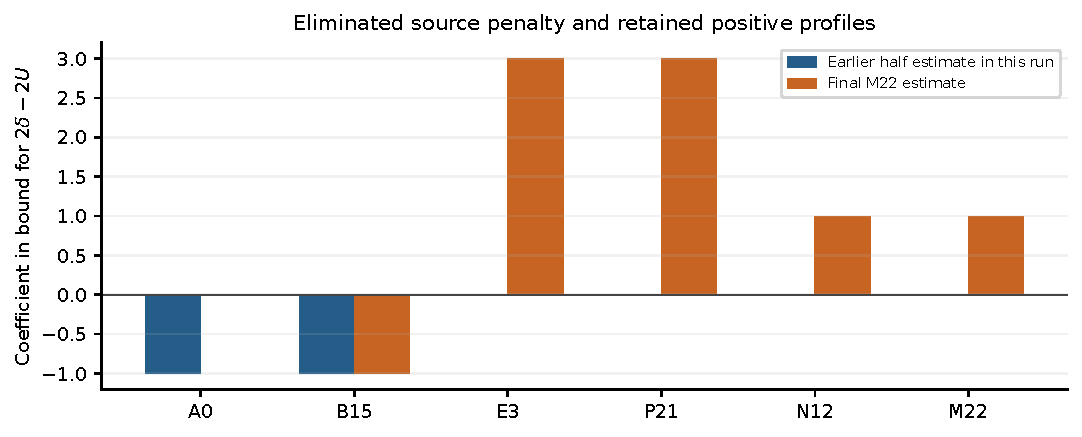
\includegraphics[width=0.95\linewidth]{new-upper-profile-coefficients.pdf}
\caption{Coefficients in the earlier half-curvature inequality and the
final all-triple global estimate developed during 5--6 October. Both
are structural bounds for actual nonparallel arrangements. The bars
compare algebraic charges of local types; they do not assert that an
arbitrary collection of those types is geometrically realizable, and
are not a comparison with an unrestricted numerical upper bound.}
\label{fig:upper-coefficients}
\end{figure}

\begin{theorem}[Componentwise N12 portfolio]\label{upper:n12-hybrid}
Under the all-triple hypothesis, let $A_s,B_s,E_s,P_s,N_s$ be the
corresponding counts in the actual component $s$. Then
\begin{equation}
 \delta\ge U+\sum_s\max\left\{
 1-A_s-\ceil{B_s/2},\;
 \ceil{\frac{3E_s+3P_s+N_s-B_s}{2}}\right\}.
 \label{upper:n12-component}
\end{equation}
This score dominates the preceding half-gain and source-free component
scores. If each component satisfies $B_s+1\le3E_s+3P_s+N_s$, then
$\delta\ge U+c$.
\end{theorem}
\begin{proof}
Localize the actual discharging and strict paid-cost arguments to each
shared-core-closed component. The component contribution $H_s$ to
$\delta-U$ is integral. The paid theorem gives
$H_s\ge1-A_s-\ceil{B_s/2}$; the source-free N12 theorem gives the other
rounded score. Take their maximum \emph{before} summing over components.
Actual component partition and side double counting prove
$\delta-U=\sum_sH_s$. The final component endpoint is
\proofref{Kobon/UpperOpenMathClosedN12Curvature.lean}{282}{\lean{certificate_n12_source_free_hybrid_component_defect}};
its dominance is proved in the same module. The sufficient positive
profile is
\proofref{Kobon/UpperOpenMathPositiveProfileComponents.lean}{43}{\lean{certificate_positive_profile_component_defect}}.
\end{proof}
The $M_{22}$ strengthening in \eqref{upper:m22-global} is currently a
\emph{global} theorem. Equation~\eqref{upper:n12-component} is the separately
completed component portfolio; no componentwise M22 extension is claimed.

\subsection{Restricted graph classes and multiplicity consequences}
\label{upper:classes}

The cap budgets themselves require no graph restriction. In the
all-triple class they give
\[
 D_1+2E_3+P_{21}\le2q,\qquad
 \delta\ge U+q-D_2+2E_3+P_{21},
\]
in \proofref{Kobon/UpperOpenMathTripleCapBudget.lean}{57}{\lean{certificate_triple_cap_budget}}.
For arbitrary multiplicities, define
$\mathcal A=\sum_{r\ge4}(r(r-4)+1)t_r$ and
$P_{\rm poor}=\sum_{v\text{ poor triple}}d(v)$, where poor means
$a\le1$ and $a+d\le2$. The mixed weighted budget is
\[
 3D_1+3q+3\mathcal A+2P_{\rm poor}\le3S,\qquad
 3\delta\ge3(U+q-D_2+\mathcal A)+2P_{\rm poor}.
\]
It is \proofref{Kobon/UpperOpenMathMixedCapBudget.lean}{53}{\lean{certificate_mixed_weighted_budget}}.
An order-four, -five or -six core contributes respectively one, six
or thirteen to $\mathcal A$. These contributions pay triple sources
without assuming that higher extremal fans are independent.

\begin{theorem}[Component and forest classes]\label{upper:class-corollaries}
For the same actual arrangement and triangle-family semantics:
\begin{enumerate}[label=(\roman*)]
\item If every core has shared-core degree at most three, then
$\delta\ge U+c+\Delta$, with arbitrary multiplicities.
\item At degree at most four, the bound is
$\delta+A_{\rm all}\ge U+c+\Delta$.
\item If each actual component has at most five vertices, then
$\delta\ge U+c+\Delta$, with arbitrary total core count and multiplicities.
\item For an actual forest, put
$\mathcal A=\sum_{r\ge4}(r(r-4)+1)t_r$ and let
$P_{\rm poor}=\sum_{v\text{ poor triple}}d(v)$. Then
$3\delta\ge3(U+c+\mathcal A)+2P_{\rm poor}$.
For an all-triple forest the separate cap budget gives
$\delta\ge U+c+2E_3+P_{21}$.
\end{enumerate}
\end{theorem}
\begin{proof}
At degree at most three, adjusted component cost is nonnegative. Its
zero case leaves a closed extremal cluster or a balanced two-cap cluster;
finite supporting geometry excludes the former and actual cycle geometry
the latter, giving strict integer cost. The degree-four version retains
full two-cap corrections. In a component of at most five vertices, a
full two-cap center and its four neighbors exhaust the component.
Opposite radial segments and ordinary cap tips block outer diagonals.
The remaining endpoint weights pay more than the center's negative
weight; mixed outer multiplicities supply their adjusted surplus.
Both antipodal and non-antipodal full two-cap shapes are handled.
These are
\proofref{Kobon/UpperOpenMathMixedDegreeThree.lean}{158}{\lean{certificate_mixed_degree_three_component_bound}},
\proofref{Kobon/UpperOpenMathMixedDegreeFour.lean}{169}{\lean{certificate_mixed_degree_four_component_bound}},
and \proofref{Kobon/UpperOpenMathMixedFiveCoreComponents.lean}{96}{\lean{certificate_mixed_five_component_bound}}.

For a forest, the actual component trees prove $D_2+c=q$.
The mixed weighted cap budget
$3\delta\ge3(U+q-D_2+\mathcal A)+2P_{\rm poor}$ gives the result.
The all-triple budget retains $D_1+2E_3+P_{21}\le2q$ before substitution
in the exact defect identity. The forest endpoints are
\proofref{Kobon/UpperOpenMathForestBudget.lean}{73}{\lean{certificate_mixed_forest_weighted_bound}}
and \proofref{Kobon/UpperOpenMathForestBudget.lean}{49}{\lean{certificate_triple_forest_bound}}.
No degree bound is required for the forest statements.
\end{proof}

A closed all-triple component of at most seven vertices contains at most
one antipodal source: two nonadjacent sources need two four-element
neighbor sets among at most five other vertices, contradicting the
at-most-two-common-neighbor theorem. The single-source charging rule gives
$\delta\ge U+\sum_s\ceil{(3E_s+2P_s-B_s)/2}$ in that class; an adaptive
maximum retains the stronger rule separately in each applicable component.
This does not remove $B_s$ or prove $\delta\ge U+c$ for all seven-core
components. The final unrestricted N12 portfolio is retained alongside
these earlier source-sensitive results.

The mixed high-multiplicity consequences also have actual formal proofs.
All multiplicities at least four imply $3T\le n(n-2)$.
At even order, multiplicities at least six give
$6T+6q\le n(2n-5)$; the sharper five-or-higher boundary theorem gives
$12T+5q+\min(q,3)\le2n(2n-5)$.
The proofs are in \lean{UpperOpenMathMultiplicity},
\lean{UpperOpenMathHighMultiplicityHull} and \lean{UpperOpenMathBoundaryBudgets}.
These restricted numerical formulas are not replacements for control of
triple and quadruple cores in the unrestricted problem.

\subsection{Parity tokens, equality attribution and remaining limits}
\label{upper:tokens}

The new parity extraction can charge every cut line in an even all-triple
arrangement, rather than only clean lines. Ordinary crossings there have
odd cardinality. The base cover either fails degree one on a transverse
segment or ends a positive triangle base at a core. Separately accounting
for these two modes gives the safe actual bound
\begin{equation}
 n\le2U+2D_1+C\qquad(n\ge4\text{ even, all cores triple}).
 \label{upper:all-line-parity}
\end{equation}
Its proof is in \lean{UpperOpenMathOrdinaryGlobalCharge}. The second $D_1$
is necessary: a four-line pencil-plus-cap witness has $U=0,D_1=1,C=2$,
so replacing $2D_1$ by $D_1$ would give the false $4\le3$.
The conjectural trade-off $n\le2U+D_1+R_c+2$, together with
$C\ge2D_1$, would yield the corrected even bound
$6T\le n(2n-5)+2$ in the all-triple class. Neither conjectural resource
rule is assumed here. Without the correction two, the known $38:450$
witness has token total 36; with correction two the rule still fails for
mixed multiplicities, where a $14:52$ witness has shortfall three.

Cl\'ement--Bader already stated that exact Tamura equality forces a
simple configuration~\cite{clementbader2007}. The quantitative penalties
and restricted equality corollaries above are independently checked
mechanisms in explicit scopes, not a claim of first discovery of that
broad conclusion. The wrong-ray/shared-apex mechanism also has prior local
arguments in Srirangam's notes~\cite{srirangam2026}; their actual fan
extraction, extended partial-fan scopes and global weighted assembly are
separate developments here. Source priority for the quantified component
penalties requires further comparison.

An exact phase-zero F\"uredi--Pal\'asti witness with eight lines has seven
triple cores, fourteen triangles and fifteen shared sides, refuting the
auxiliary general shortcut $D\le2q$. At eighteen lines its exact profile
is $q=46,D_1=15,D_2=105$. An eleven-line witness has adjacent order-five
extremal full fans, so higher extremal independence is also false.
These retained exact external counterexamples invalidate specified
charging shortcuts, not the final numerical conjectures in which those
shortcuts were used. A seven-vertex kernel-checked abstract half-charging
example is sharp for its finite relaxation but unrealizable: its two
sources would have the same four neighbors. It therefore identifies
missing geometry rather than sharpness for real Kobon arrangements.

A finite projective chart theorem now removes parallel pairs while
preserving a chosen finite set of actual bounded triangles. It requires
distinct projective lines and nonparallel supporting pairs for each
triangle; the old polynomial predicate alone is not used on a parallel
support pair. The endpoint
\proofref{Kobon/OpenMathParallelElimination.lean}{199}{\lean{arbitrary_iff_lowerBound}}
links the arbitrary and nonparallel lower-witness models. Class properties
and local profile counts must still be checked in the transformed chart;
this does not silently extend an all-triple theorem to every parallel
arrangement. The remaining general upper task is mathematical control
of residual profiles and the ordinary-end token trade-off, rather than
unfinished extraction of the fans already used above.

\section{Exact translation germs and local resolution losses}
\label{sec:surgery}

A small perturbation of a multiple point can create a tiny triangle and
destroy distant old cells simultaneously. This section gives an exact
description of that wall crossing. It does not assume that smoothing
preserves or increases the triangle count.

\subsection{Simultaneous classification by affine coefficients}

Translate one indexed line parallel to itself, writing its equation as
$a_px+b_py=c_p+\varepsilon$ and leaving the others fixed. Pairwise
nonparallelism is preserved. Every determinant nondegeneracy test and
oriented half-plane test in the triangle certificate has the form
$u+v\varepsilon$: multilinearity and the single changed constant term
exclude higher powers. For positive sufficiently small $\varepsilon$,
\[
 u+v\varepsilon\ge0\quad\Longleftrightarrow\quad
 (u>0)\ \text{or}\ (u=0\text{ and }v\ge0),
\]
with analogous rules for nonpositivity and nonzero tests. A
\emph{triangle germ} is the static conjunction of these coefficient
conditions for one ordered supporting triple.

\begin{theorem}[Exact eventual translation count]\label{surgery:germs}
For any finite pairwise nonparallel arrangement and one translated line,
there is $\eta>0$ such that, simultaneously for every supporting triple
and every $0<\varepsilon<\eta$, the moved triangle predicate is equivalent
to its germ. Let $T(0)$ be the old count, and let $\mathrm{born}$ and
$\mathrm{lost}$ count germs absent from the old triangle set and old
triangles absent from the germ set, respectively. Then throughout that
interval,
\begin{equation}
 T(\varepsilon)+\mathrm{lost}=T(0)+\mathrm{born}.
 \label{surgery:birth-loss}
\end{equation}
\end{theorem}
\begin{proof}
For each affine test with nonzero constant coefficient, choose a positive
threshold preserving its sign; zero constants are decided exactly by the
linear coefficient. There are finitely many tests, supporting triples
and transverse lines. Intersect their positive neighborhoods to obtain
one simultaneous threshold. Nondegeneracy and the common half-plane
tests then give exactly the original geometric certificate predicate.
The finite set identity follows by partitioning both the old and germ
sets into their intersection and their differences. These are
\proofref{Kobon/OpenMathTranslationGerms.lean}{205}{\lean{simultaneous_triangle_stability}}
and \proofref{Kobon/OpenMathTranslationCounting.lean}{98}{\lean{translated_birth_loss_identity}}.
The lower-bound wrappers supply actual real-line witnesses from germ
counts, rather than treating a formal count as a geometric oracle.
\end{proof}

Explicit corner-incidence conditions make every old triangle's zero
side tests stationary; their other signs persist. This proves no loss
and a one-triangle gain when a new germ is present, in
\proofref{Kobon/OpenMathTranslationRetention.lean}{98}{\lean{germ_gain_one}}.
If there is exactly one concurrent supporting triple and no other line
through its center, translating one of its supports creates exactly one
tiny-triangle germ. Other new germs would have to be old degenerate
supporting triples and are excluded by uniqueness. Consequently
\begin{equation}
 T(\varepsilon)+\mathrm{lost}=T(0)+1.
 \label{surgery:isolated}
\end{equation}
This is
\proofref{Kobon/OpenMathIsolatedTripleResolution.lean}{78}{\lean{isolated_resolution_identity}},
using the local birth theorem in \lean{OpenMathTripleBirth}.
The loss set remains the \emph{global} germ difference. These theorems
use only the standard logical axioms and permit arbitrary finite order.

\subsection{A four-line counterexample to a stated half-plane yield}
\label{surgery:four}

Liu's versioned desingularization preprint, Theorem~1.1 on printed page
2, states a formula $T(A')=T(A)+1-\tau_i$, with $\tau_i$ defined by
old triangle interiors lying in the selected open half-plane
\cite{liuDesingularization2026}. Its hypotheses include one isolated
triple point and otherwise ordinary vertices. The following example
satisfies those hypotheses:
\begin{equation}
 y=0,\qquad y=x,\qquad y=-x,\qquad 2x+y=2.
 \label{surgery:four-lines}
\end{equation}
Index these supports $0,1,2,3$. The old triangular cells have supports
$013$ and $023$, and both interiors satisfy $x-y>0$.
Move support 1 to $y=x+\varepsilon$, so its motion is into $x-y<0$.
The stated half-plane count is zero. Yet for every $0<\varepsilon<1$
the moved arrangement has exactly two triangles, with supports $012$
and $023$. One old cell is lost and one is born; the proposed yield
would instead predict three triangles.

This is an interval counterexample within the formula's stated scope,
not a criticism of unrelated results in the preprint. Completeness of
the old and moved support lists, the unique triple, the whole parameter
interval, and positivity throughout the old triangle interiors are
proved in
\proofref{Kobon/OpenMathFourLineResolution.lean}{190}{\lean{halfplane_yield_fails}}.
The exact germ identity~\eqref{surgery:birth-loss} accounts for the loss
without replacing it by the half-plane count.

\subsection{Three losses and a reversed gain of two}
\label{surgery:six}

A second arrangement is
\begin{equation}
 y=0,\quad y=x,\quad y=-x,\quad x+2y=3,\quad
 -2x+y=2,\quad x+4y=-4.
 \label{surgery:six-lines}
\end{equation}
It has one concurrent triple and six old triangles. For every
$0<\varepsilon<1/100$, replacing the first line by $y=\varepsilon$
retains all six and creates one, whereas replacing it by
$y=-\varepsilon$ destroys three old triangles and creates one. The
old affected cells occupy alternating radial sectors $0,2,4$.
\begin{table}[tb]
\centering\small
\begin{tabular}{@{}lrrrr@{}}
\toprule
Motion & Old count & Lost & Born & Moved count\\
\midrule
Four-line positive resolution & 2 & 1 & 1 & 2\\
Six-line upward resolution & 6 & 0 & 1 & 7\\
Six-line downward resolution & 6 & 3 & 1 & 4\\
\bottomrule
\end{tabular}
\caption{Complete real-parameter interval counts for the displayed
arrangements. Birth and loss refer to supporting-triple sets, and the
interval conclusions are Lean theorems.}
\label{surgery:counts}
\end{table}
The complete support classification is proved in
\proofref{Kobon/OpenMathSixLineResolution.lean}{557}{\lean{up_count}}
and \proofref{Kobon/OpenMathSixLineResolution.lean}{566}{\lean{down_count}}.
The reverse collapse from the downward arrangement to the singular
one gains two triangles, in
\proofref{Kobon/OpenMathSixLineResolution.lean}{570}{\lean{reversal_gain_two}}.
Thus neither a universal cap of two destroyed cells nor a one-unit
reverse yield is valid in this scope. The positive direction also shows
that resolution can be useful when a genuine global retention proof
accompanies its local birth certificate.

\section{Exact certificates, external reproduction, and unsuccessful searches}
\label{exp:section}

The experimental program serves two purposes: producing concrete coordinate
witnesses for lower bounds, and identifying which proposed general arguments
survive exact checks. These purposes require different standards of evidence.
A successful coordinate witness proves an existential lower bound at its
specified order. A failed search ordinarily proves neither an upper bound nor
the nonexistence of a better construction. This section records both positive
and negative outcomes without merging their logical scopes.

\subsection{From a numerical proposal to an exact geometric witness}

The stored coordinates use the convention $a_ix+b_iy=c_i$, with rational or
integer coefficients. Each line is normalized to a primitive integer triple.
Pair intersections are computed as homogeneous integer triples, normalized
with a positive final coordinate. Consequently, collinearity, concurrence,
parallelism, and comparisons along a supporting line can all be tested without
floating-point tolerances.

Two independently implemented counters are used. The first sorts the distinct
intersection vertices on each line and constructs the graph of elementary
bounded segments; a three-cycle supported by three different lines is a
triangular cell. The second enumerates support triples and tests whether every
other line has a common weak sign at their three vertices. Nonzero area and
the distinction between open interiors and boundaries are checked explicitly.
Where a complete independent verification is reported, both counters agree on
the triangle set, not merely on a rounded area or a visual estimate. The Lean
geometric soundness theorem provides a third, logically separate link from
accepted coordinate predicates to real affine triangles.

Numerical optimization is used only to propose coordinates or rank candidate
chambers. A proposal is rationalized and recounted before promotion. In the
phase/chart experiments, progressively finer integer scales were accepted only
when the entire exact triangle set and simplicity were retained. Such a finite
acceptance does not prove that an arbitrary rounding of an irrational
construction is valid. The real all-order theorem for $\G$ has its own
determinant, trigonometric, and counting proof.

The released catalog contains 138 distinct promoted coordinate identities.
Several identities can occur at the same order and triangle count, and an
identity may have several repository source paths. Thus 138 is a catalog size,
not a count of new records or independent discoveries. The complete catalog
in Table~\ref{exp:catalog} includes simple versus nonsimple status, provenance
collections, and coordinate-hash prefixes; its machine-readable companion
records full hashes, source paths, and theorem modules. The finite Lean
certificates use native evaluation where indicated. This trust boundary is
broader than that of the universal construction, whose proof uses only Lean's
standard logical axioms.

\subsection{Finite improvements relative to the retained collection}

The phase and affine-chart work raised the preceding saved values at eleven
orders:
\[
\begin{array}{c|rrrrrrrrrrr}
n&39&47&48&51&53&54&55&59&60&99&195\\\hline
\text{previous}&469&690&720&817&884&918&954&1102&1140&3169&12481\\
\text{current}&470&691&721&818&885&919&955&1103&1141&3170&12482
\end{array}
\]
Each row is an improvement over the project's preceding retained coordinate
catalog. The underlying trigonometric family is due to
F\"uredi--Pal\'asti~\cite{furedipalasti1984}; these comparisons do not establish
numerical first priority. The general formula $\G$ now explains all eleven
displayed counts. The first projective search reached $47:691$ after 11,264
proposals; the subsequent exposed-cap description replaced that search by a
direct construction and an all-order proof.

The earlier OEIS-attributed values $28:238$, $30:275$, and $34:357$ remain
independently certified~\cite{oeisA006066,zarzuelo2026}. The drawings in this
paper render the currently retained exact witnesses, obtained by exterior
extension of retained odd-order inputs. They are not asserted to be literal
reproductions of the March diagrams. Likewise, the historical inventory in
Table~\ref{exp:historical} preserves earlier outputs without upgrading every
original derivation to a completed general theorem.

The current strongest saved simple and classical coordinate counts for every
$3\leq n\leq60$ appear in Table~\ref{exp:finite-table}. An absent entry in the
explicit OEIS table is recorded as a dash. Absence from that table is not
evidence that a value is absent from the literature; conversely, a coordinate
certificate does not establish optimality without an upper theorem covering
the same arrangement class.

\subsection{Independent reproduction of external constructions}

The current Parpalak--Utkin coordinate gallery~\cite{parpalakutkin2026} supplied
exact witnesses at
\[
\begin{gathered}
8:15,\quad14:54,\quad20:117,\quad26:204,\quad32:315,\\
36:402,\quad38:450,\quad42:553,\quad46:667,\quad50:792.
\end{gathered}
\]
Both independent counters reproduced their triangle sets. These witnesses
retain their source attribution; in particular, the eight-line numerical
value has older discovery priority than the coordinate gallery. Their addition
to this repository improves its verified coverage, not the discoverer's
claim to the numbers. The inspected gallery snapshot is commit
\texttt{feae4f5571a988a3ed45bd26a36259ebb7d7d3d2}.

All fifteen of Andrea Maiorana's published $14:54$ coordinate
configurations~\cite{maiorana2026} were also independently checked. Fourteen
have exactly two triple points, and one has four; none has a parallel pair.
The source snapshot is commit
\texttt{e47c7cfd9661e54d29befb83118bf83d5f804028}. Its CC BY 4.0 licence,
original coordinate files, and source attribution are retained. Added wrappers
record counts and verification metadata. This reproduction imports no claim
that a simple-arrangement upper theorem applies to these nonsimple witnesses.

These examples also expose a concrete limitation of smoothing. In Maiorana's
first example, the triple supports are $\{0,4,10\}$ and $\{0,11,12\}$.
Independently shifting the offsets of lines 4 and 11 by $\pm1/1000$ realizes all
four local resolution choices while preserving every originally nonzero
determinant sign. The resulting triangle counts are $52,52,53,52$, all below
54. Thus the proposed nondecreasing local smoothing strategy fails even when
the local sign choices are independently realizable by straight lines. The
argument identifying these sign choices with all sufficiently small local
resolutions is an ordinary finite sign-stability argument, not a completed
Lean theorem.

For the gallery's collinear-core examples at orders
$8,14,20,26,32,38,50$, all 132 recorded local resolutions were realized by
exact private-line offsets. Their respective best simple counts were
$14,51,114,203,313,448,791$. In particular, a universal claim that resolving
such a core loses at most one triangle is also false. Figure~\ref{fig:external-comparison}
separates these finite obstructions from any general upper-bound assertion.

\begin{figure}[tbp]
  \centering
  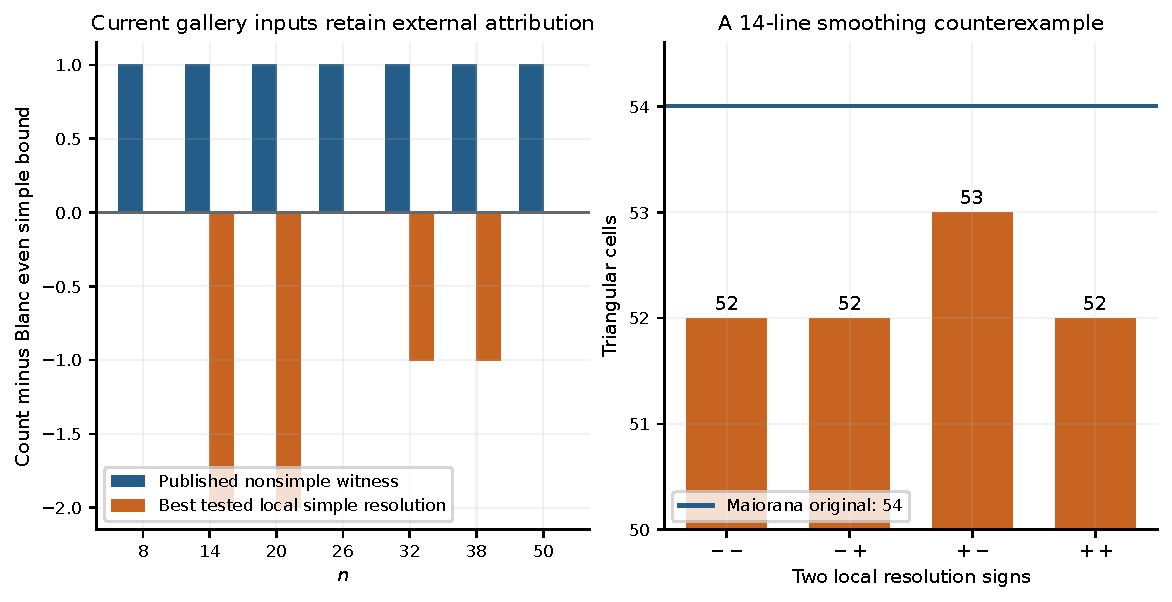
\includegraphics[width=\textwidth]{figures/external-comparison.pdf}
  \caption{Exact local-resolution tests on attributed external constructions.
  Left: Parpalak--Utkin gallery witnesses and their best tested simple local
  resolutions, measured relative to Blanc's even simple-arrangement polynomial;
  the eight-line value has older priority. Right: all four local resolutions of
  Maiorana's two-triple-point $14:54$ example. The original arrangements are
  nonsimple, so exceeding the simple polynomial is consistent. These are
  smoothing obstructions, not upper bounds for the classical problem.}
  \label{fig:external-comparison}
\end{figure}

\subsection{Projective charts, algebraic curves, and chamber searches}

Projective geometry provides a useful global neighborhood: changing the line
at infinity moves all lines together and may bound formerly unbounded
triangular faces. It can also lose bounded cells. For the exact saved
$81:2132$ and $161:8532$ hybrid arrangements, the projective triangular-face
census already equals their bounded-cell count; a chart change alone cannot
increase those particular counts.

Exact rational linear-arithmetic searches give sharper restrictions for some
fixed configurations. The nine-line half-phase rational arrangement has 21
projective triangular faces, but the recorded QF\_LRA solver result rules out a
chart retaining all 21. Similar fixed-seed tests find no gain for the tested
half-phase arrangements at $14,20,26,44$, and no chart retaining all 471
projective triangles of the saved $39:470$ witness. For a nonuniform cubic
48-line seed with 724 projective triangles, 2,903 exact linear-arithmetic checks
rule out 722 bounded triangles within the tested chart-retention formulation.
These are exact-solver results about specified rational seeds. Their UNSAT
certificates have not been independently checked in Lean, and they are not
global upper bounds at those orders.

The algebraic-curve direction tested both nodal-cubic angle perturbations and
torsion cosets on real elliptic curves. A larger projective face count did not
automatically produce a better affine construction. For the better two-real-
component elliptic examples, the projective, original affine, and best found
affine counts were respectively
\[
\begin{array}{c|rrrr}
n&42&48&54&60\\\hline
\text{projective}&550&724&922&1144\\
\text{original affine}&538&710&907&1127\\
\text{best found affine}&539&712&908&1129
\end{array}
\]
All fall below the corresponding retained affine bounds. The chart scans at
54 and 60 had 90-second limits. Numerical ranking and bounded running time
preclude a global nonexistence inference.

Oriented-matroid mutations and kinetic chamber sweeps addressed a different
limitation: moving inside a fixed projective type cannot create new
projective triangular faces. The mutation searches changed determinant signs,
using linear-programming realization where appropriate. Kinetic sweeps varied
many offsets, or both slopes and offsets, and visited concurrency events along
selected rays. Their event counts are not counts of all realizable order
types, and unsuccessful floating rays were discarded. Figure~\ref{fig:negative-searches}
records effort without treating heterogeneous search units as comparable
coverage measures.

\begin{figure}[tbp]
  \centering
  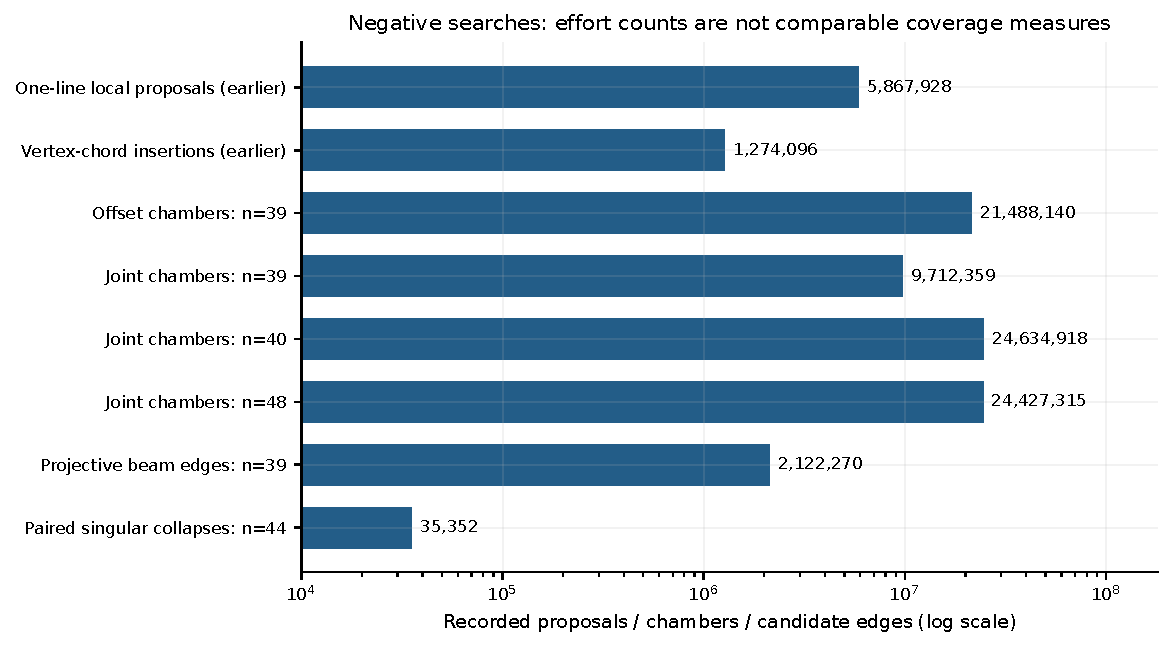
\includegraphics[width=\textwidth]{figures/negative-searches.pdf}
  \caption{Selected unsuccessful searches, with their recorded units.
  Proposal, chamber, and candidate-edge totals describe different search
  neighborhoods. They do not measure exhaustive coverage, justify an upper
  bound, or rank the mathematical promise of the methods. All proposed
  improvements would require subsequent exact geometric verification.}
  \label{fig:negative-searches}
\end{figure}

The final 39-line projective beam examined 2,122,270 candidate edges through
4,559 states without exceeding 470 affine or 471 projective triangles, even
at its combinatorial scoring stage. The 48-line LP walk accepted 471 mutations
out of 511 attempts and retained 721 affine and 724 projective triangles.
At 44 lines, singular-boundary searches included 35,352 paired collapses;
the retained beam checkpoint had 771 states and 446,422 candidate edges,
without exceeding 608. An unfinished round was discarded. These results
motivate a change of neighborhood or a structural argument rather than
repeating the same local searches.

Other bounded approaches included Fourier deformations (2,687,600 proposals
in one 39-line run), partial deletions from BBL constructions, and constrained
tangent-grid transfer by LP/MILP. The tested optimal 23-line chart transfers
did not admit a positive-margin realization on the desired grid; a constrained
near-optimal search gave 144 triangles, below a separately known compatible
145. None of these observations proves nonexistence of another compatible
seed or a different successful deletion pattern.

\subsection{A proved algebraic obstruction to tangent-grid transfer}
\label{exp:grid-obstruction}

The October search connects oriented-matroid sign constraints, linear
programming duality and exact algebraic number arithmetic. For the
reciprocal-coordinate lines $x-v_i y=a_i$, a prescribed determinant
sign becomes a strict linear inequality in the unknown reciprocal
slopes. Write
\begin{equation}
 D_{ijk}=(a_j-a_k)v_i+(a_k-a_i)v_j+(a_i-a_j)v_k.
 \label{exp:linear-determinant}
\end{equation}
Once the intercepts are fixed, feasibility is a linear sign problem,
even though the intercepts themselves are algebraic.

\begin{lemma}[Positive-dependence obstruction]\label{exp:farkas}
Let $A_i\in\R^d$ and let $\lambda_i\ge0$, with at least one
$\lambda_i>0$, satisfy $\sum_i\lambda_i A_i=0$. There is no $v\in\R^d$
with $A_i\mathbin{\cdot}v>0$ for every $i$.
\end{lemma}
\begin{proof}
Taking the scalar product with $v$ makes the left side a positive
weighted sum, but the assumed vector identity makes it zero. This
classical strict alternative is formalized by
\sourcefile{Kobon/StrictLinearCertificate.lean}{\lean{homogeneous_infeasible}}.
The formal theorem also provides an affine form for nonhomogeneous
strict systems.
\end{proof}

Set $t=\tan(\pi/20)$. Its exact algebraic specification is
\begin{equation}
 p(t)=t^4-4t^3-14t^2-4t+1=0,
 \qquad \frac3{20}<t<\frac{17}{100}.
 \label{exp:quartic}
\end{equation}
The quintuple-angle identity with $\tan(5\pi/20)=1$ gives
$(t-1)p(t)=0$; the interval excludes $t=1$. Monotonicity on the interval
identifies the intended root. \lean{BBLTangentAlgebra} proves the
quartic, root interval and uniqueness; \lean{BBLTangentValues} proves
that its explicit cubic power-basis expressions are the actual nine
values $\tan(k\pi/20)$ for $1\le k\le9$. Thus replacing trigonometric
numbers by algebraic expressions does not insert a numerical guess.

Use the actual 20-intercept grid
\[
 a_j=\begin{cases}
 -\tan((9-j)\pi/20),&0\le j<9,\\
 -\varepsilon,&j=9,\\
 \varepsilon,&j=10,\\
 \tan((j-10)\pi/20),&11\le j<20.
 \end{cases}
\]
The following ten prescribed signs are impossible.

\begin{theorem}[One exact tangent-grid obstruction]
\label{exp:actual-grid-obstruction}
For every real $\varepsilon$ and every real vector
$(v_0,\ldots,v_{19})$, at least one row of
Table~\ref{exp:ten-signs} fails the strict inequality
$s_iD_{j_i k_i\ell_i}>0$.
\end{theorem}

\begin{table}[tb]
\centering\small
\begin{tabular}{@{}cll@{}}
\toprule
Support triple & $s_i$ & Positive multiplier $\lambda_i(t)$\\
\midrule
$(0,6,15)$ & $-1$ & $-20t^3+120t^2+300t-40$\\
$(0,7,13)$ & $+1$ & $-8t^3+24t^2+96t+8$\\
$(0,8,14)$ & $-1$ & $-45t^3+205t^2+555t-35$\\
$(0,13,19)$ & $+1$ & $-16t^3-6t^2+40t+2$\\
$(3,6,8)$ & $+1$ & $20t^3-100t^2-220t+100$\\
$(3,11,15)$ & $-1$ & $20t^3-120t^2-220t+200$\\
$(3,13,17)$ & $+1$ & $20t^3-150t^2-300t+130$\\
$(7,11,13)$ & $+1$ & $-60t^3+240t^2+860t+320$\\
$(8,14,17)$ & $-1$ & $-105t^3+455t^2+1275t-45$\\
$(8,15,19)$ & $-1$ & $36t^3-188t^2-452t+124$\\
\bottomrule
\end{tabular}
\caption{An explicit positive linear-dependence certificate. Indices are
zero-based intercept indices. The rows use eleven distinct intercepts
and avoid the two exceptional central indices. Each column of the
weighted signed coefficient matrix vanishes modulo $p(t)$.}
\label{exp:ten-signs}
\end{table}

\begin{proof}
For each row define $A_i$ to be the coefficient vector of $s_iD$ in
\eqref{exp:linear-determinant}. All ten displayed multipliers are
positive throughout $3/20<t<17/100$, by rational polynomial inequalities.
Using the proved power-basis expressions for the tangents, expand
$\sum_i\lambda_i(t)A_i$ one column at a time and reduce modulo $p(t)$.
Every column is zero. The two central columns vanish because none of
the ten supports uses indices 9 or 10. Lemma~\ref{exp:farkas} gives a
contradiction. The exact source contains the polynomial multiple of
$p$ for every nontrivial column, so the computation is reproducible
without a floating-point linear solver. The declarations
\proofref{Kobon/BBLGridObstruction.lean}{240}{\lean{actual_grid_infeasible}}
and
\proofref{Kobon/BBLGridObstruction.lean}{263}{\lean{actual_grid_orientation_impossible}}
prove this for the actual tangent grid using only standard logical
axioms.
\end{proof}

This excludes one explicit orientation system with arbitrary reciprocal
slopes and every real central parameter. It does not classify all
21-line arrangements. An independent exact interval Gaussian-elimination
check also proves persistence under independent perturbations of radius
$10^{-3}$ on the eleven used intercepts. That robustness calculation is
external exact evidence, not part of the Lean theorem above.

\subsection{The full supplied affine-class obstruction census}
\label{exp:affine-census}

Parpalak--Utkin's enumeration separates projective and Euclidean
classes~\cite{parpalakutkinEnumeration2026}. This distinction changed
the scope of the search. The first checker verified 366 exact polynomial
certificates for eighteen supplied projective representatives on
$0<\varepsilon<1/25000$. A projective representative alone does not
exhaust its affine cases: a choice of infinity support matters. That
initial census was therefore insufficient for a complete affine claim.

The corrected checker expands all 236 supplied Euclidean classes and
all 21 choices of distinguished support. It validates 3,765 exact
polynomial dependencies and 15,060 reflected or reoriented variants,
covering all $236\cdot21=4,956$ class/support cases with no missing case,
for
\begin{equation}
 0<\varepsilon<1/2{,}000{,}000.
 \label{exp:census-interval}
\end{equation}
Every certificate is a positive linear contradiction of the form above,
so it excludes arbitrary, even parameter-dependent, reciprocal slopes.
The small positive interval is a uniform bound for this finite corpus;
it is not the unrestricted all-real parameter assertion proved for the
single ten-sign representative.

The logical dependencies remain separate. The completeness of the
classification is supplied by Parpalak--Utkin and its dataset. The
present independent checker validates the listed exact certificates,
the class/support coverage and the explicit symmetries. It does not
rerun their full enumeration inside Lean. The resulting exclusion of a
perfect 21-line seed on this prescribed saturated grid and interval is
therefore computer-assisted mathematics with an external classification
input. Only Theorem~\ref{exp:actual-grid-obstruction} is a complete
representative Lean obstruction. Other grids, larger seeds, nonsimple
arrangements and other construction methods remain unrestricted by this
census.

\subsection{New bounded searches and their exact outcomes}

The 2 October work also tested finite neighborhoods selected to change
features that the earlier chart-only searches preserved. None produced
a new numerical lower-bound record. The exact positive and negative
results are summarized below; completed enumeration of a listed
neighborhood does not imply enumeration of all arrangements.

\begin{table}[tb]
\centering\small
\begin{tabularx}{\linewidth}{@{}P{0.29\linewidth}XP{0.24\linewidth}@{}}
\toprule
Search & Result & Limitation\\
\midrule
Deletions from a 49-line seed & Best retained values $48:721$, $47:677$,
$46:637$, $45:598$. & The tested deletion neighborhood only.\\
57-line MILP deletions & Incumbents $56:990$, $55:939$, $54:887$,
$53:837$. & Timed runs; incumbents are not proved maxima.\\
All 9,180 tested chords of a 17-line seed & Best 18-line output has 93
triangles. & Chords of one seed.\\
407,253 vertex-pair insertions at 43 lines & Best 44-line output has
607 triangles, below retained 608. & The stated insertion neighborhood.\\
Singular 16-to-18 insertion & Best recorded count 89. & No global
exclusion.\\
39-pseudoline straightening & Exact realizations with 353 and 358
triangles. & Neither a record nor a proof of nonstretchability.\\
Perfect 21-line grid fit & Exact affine-class obstruction census. & The
prescribed grid, interval and supplied classification.\\
49-line grid fit & Uniform 767-cell certificate and full visible boundary.
& Full Lean base and odd/even instantiation now completed.\\
\bottomrule
\end{tabularx}
\caption{The added research directions and their actual conclusions.
The 49-line positive result is compared with its known BBL numerical
family in Section~\ref{fam:seed49}.}
\label{exp:october-searches}
\end{table}

The methodological connection to recent automated mathematical search
is a separation of proposal, evaluation and proof, also emphasized by
Georgiev, G\'omez-Serrano, Tao and Wagner~\cite{georgiev2025}. Here a
numerical optimizer proposes a coordinate or dual vector; exact
arithmetic certifies the finite claim; the symbolic construction or
obstruction explains which statements hold uniformly. Their paper is
methodological context, not evidence that Kobon has already been solved.
The author's other construction projects motivated preserving an
iterable invariant and exploiting symmetry orbits; none of their
unrelated theorems is imported as a Kobon lemma.

\subsection{Cap-cone searches and the promoted 61 visibility resource}
\label{exp:cap-cone}

The 5--6 October search uses a larger feasible region than the fixed
orientation cell. For ordered axis intercepts $a_i$, write each other
line as $x-u_i y=a_i$ and fix the above/below pattern of consecutive
axis caps. For each adjacent pair $(j,j+1)$ and every other support $r$,
the determinant wall is
\[
 (a_{j+1}-a_r)u_j+(a_r-a_j)u_{j+1}+(a_j-a_{j+1})u_r.
\]
The cap conditions are linear inequalities in the reciprocal slopes.
\proofref{Kobon/OpenMathAxisCapCone.lean}{218}{\lean{capRegion_iff}}
proves their equivalence to the actual empty nondegenerate caps with the
fixed strict orientation pattern, and
\proofref{Kobon/OpenMathAxisCapCone.lean}{57}{\lean{capRegion_convex}}
proves convexity. Interpolation preserves the axis caps; it need not
preserve simplicity or other triangle cells while crossing concurrence
or parallel facets.

Reduced-row LP walks use adjacent crossing-order constraints, initially
1,219 independent walls in place of 35,990 full simplicity conditions,
and recount every realized row order. Deeper and heap walks permit
temporary triangle losses. The nonlocal cap-cone ray method moves all
60 reciprocal slopes, processes concurrence and parallel events, and
independently recounts selected chambers. Its promoted outcome is the
1190-triangle, 29-visible-pair seed of Theorem~\ref{fam:61-complete}.
More than a million explored facet crossings are discovery coverage;
they are not a global 1190-triangle ceiling, and crossings may repeat.
Rejected floating discrepancies remain in the reports. Every promoted
coordinate proposal requires a whole true-tangent interval certificate
and a fresh dependent Lean replay.

\subsection{Bounded screens, transport diagnostics and a scoped dual}
\label{exp:october-five-searches}

The unsuccessful directions are retained because each excludes a
specific proposed route or suggests a different invariant. Their
scope is the supplied types, charts, parameters or finite sample.
\begin{longtable}{@{}P{0.29\linewidth}P{0.64\linewidth}@{}}
\caption{Additional bounded research of 5--6 October. Numerical failure
is not a theorem of geometric nonexistence.}\label{exp:bounded-five-table}\\
\toprule Route & Recorded outcome and boundary\\\midrule\endfirsthead
\toprule Route & Recorded outcome and boundary\\\midrule\endhead
\bottomrule\endfoot
Central-slope scaling & Eight powers at four exact epsilon samples each
were weaker than the 1182 fixed-slope small-epsilon seed. The full
reciprocal-slope refit supersedes this 32-case screen.\\
Phase-shifted affine charts & 120 sampled charts at each of 16 even
orders from 12 through 90 did not improve their existing count. This
does not exhaust all projective charts.\\
Other 61 affine types & Every normal sector of the supplied 1189 type
has at most 28 visible pairs. The 1187 type cannot improve 1218 even
with all 30 pairs. These conclusions concern those types.\\
Deletion and random thinning & Averaged one-line deletion from a dense
BBL family gives the preceding $G$ value; the multi-line average has
leading $n^3/(3N)$. Exact 61-certificate incidence transport through
depth six gives minimum incidence $q-7$, whose deletion count is four
below $G(q)$. No arbitrary deletion theorem is asserted.\\
Visibility transport & Independently recounted rational diagnostics at
61, 121 and 241 give 1190, 4790 and 19190 cells and best sector resources
28, 58 and 118 for the original seed. Those finite rational proposals
are separate from the true-tangent uniform theorem and the new 29-pair seed.\\
41/45 fixed-type and jet fits & The alternative chart runs tested
37/42 and 24/46 charts, visiting 1477 and 1059 unique sign cells.
First- and second-order parameter jets tested eight source axes per
order. No robust positive-margin fit was found.\\
Optimal31 recharting & All 29 original-infinity saturated axes of the
published 299-cell input failed the floating margin screen. New infinity
charts were recounted before fitting; no whole-interval uniform seed
was promoted. A lower finite count is relevant only if compatibility
improves the recursive successor.\\
Singular and retained-backbone probes & Raising existing cores,
pencil slides, corridor grids, even corridor lifts and larger backbone
variants did not produce a promoted improved compatible seed. Fixed-axis
nesting and insertion failures concern those supplied types.\\
Other finite neighborhoods & Dual mutations, elliptic cosets, harmonic
and offset probes, and local chamber searches retain their exact
parameters and finite outcomes. Neither LP failure nor a sampled
maximum certifies a general upper bound.\\
Phase-zero infinitesimal resolutions & The modeled old-triangle
conflict graph has a perfect matching in 56 tested orders from 8--60
and at 99, 120, 195. Even independent modeled local choices retain at
most half the old cells there. This is a finite combinatorial screen,
not an all-order Lean perturbation obstruction.\\
\end{longtable}

A stronger kind of negative evidence is available for one prescribed
41-line cell. Eleven positive rational Farkas weights were verified by
exact arithmetic on the exported axis0/original-infinity normalized
constraints. Actual tangent intervals were independently checked using
rational arctangent-quarter inequalities and the proved pi band.
They exclude the required weighted budget for every positive epsilon
up to approximately $0.01401555$, even for epsilon-dependent reciprocal
slopes. This is a metric obstruction for that cell, not an exclusion of
all 41-line types. The generic coefficient-box/small-parameter separation
theorem is
\proofref{Kobon/OpenMathParametricDual.lean}{59}{\lean{no_budget}},
with standard logical axioms. The concrete 41-line certificate remains
exact external evidence pending its own concrete Lean replay.

The complete experiment records are under
\sourcefile{research/openmath-seven-hour-2026-10-05/constructions/README.md}{construction evidence},
\sourcefile{research/openmath-seven-hour-2026-10-05/seed_search/STRUCTURAL_PROBES.md}{structural seed probes},
and the pinned \sourcefile{research/openmath-seven-hour-2026-10-05/corpus/INDEX.md}{corpus proof map}.
The OpenMath source inventory pins the contestant repositories and judging
archive~\cite{poola2026,srirangam2026,openmathJudging2026}.
Successful contestant inputs keep their attribution. The external
39-line 471-cell replay recorded there is separate from this repository's
inherited 138-certificate catalog and is not claimed as this author's result.

\subsection{Reproduction and presentation audit}

The research registers preserve source snapshots, experiment scripts, seeds,
parameters, checkpoints, and exactness limits~\cite{zarzueloRepository}. The
paper's figures are original vector renderings, not copied source figures.
The generator \texttt{paper/scripts/generate\_figures.py} reads the research
data without modifying it and exports PDF figures, PNG previews, LaTeX tables,
and machine-readable rendering data. The figure manifest records input-file
hashes and the mathematical status of each caption. Geometric views recompute
their exact triangle lists before converting coordinates to floating point
for display. Cropped detail panels and independent affine axis rescaling are
explicitly labeled; lengths and angles are not inferred from those views.

The appropriate experimental conclusion is therefore selective. Exact
coordinates have strengthened the retained lower-bound envelope and revealed
specific failed construction rules. The successful universal advance comes
from replacing a numerical chart search by a geometric exposure proof and an
all-order count. The remaining negative searches narrow useful next steps,
but they do not solve the general optimization problem.

\section{Formal verification and reproducibility}\label{sec:formalization}

\subsection{The verified snapshot}

The mathematical snapshot used by this edition is repository commit
\nolinkurl{f44f23ee062a255f5cad7d39188fd55c0feb83a8}. It pins Lean 4.31.0 and Mathlib commit
\nolinkurl{fabf563a7c95a166b8d7b6efca11c8b4dc9d911f}. The source-linked
proof map and accompanying release record identify the exact audit and
compiler logs. Verification statements concern that collection of
declarations and coordinates; they do not assert that every research
claim or external dataset has been formalized.

The 5--6 October release record covers 638 active modules: 265 compiled
during that run and 373 unchanged source/import closures reused from
the completely verified baseline \nolinkurl{112409e2c62b78ecff7adcad49f1e014ea5f0773}.
Its fresh whole-project axiom audit inspects 9,058 theorem declarations:
8,046 use only standard logical axioms and 1,012 additionally depend
on explicit finite native-evaluation roots. This incremental replay is
distinguished from a clean build by the usual CI verifier. The counts
describe the complete retained library, including auxiliary and generated
declarations, rather than 9,058 independent new discoveries. The inherited
coordinate catalog still contains 138 identities, of which 104 are simple;
the independent new uniform seed modules have their own proof provenance.

\subsection{Three proof and computation boundaries}

\paragraph{General symbolic proofs.}
The arbitrary-order construction, generic closed BBL recursion,
quantitative successor and iteration, actual structural upper bounds,
translation germ theorems, interval loss-rule counterexamples and
representative grid obstruction use the usual Lean axioms
\lean{propext}, \lean{Classical.choice}, and \lean{Quot.sound}.
No unproved geometric construction is installed as an axiom. Their
conclusions are not extrapolated from a finite range of successful
tests. Lean and Mathlib provide the real analysis, finite combinatorics
and algebra used in these proofs~\cite{lean4,mathlib}.

\paragraph{Finite certificates.}
Large coordinate checks use \lean{native_decide}, which trusts Lean's native compiler and runtime in addition to the ordinary logical kernel interface. The general certificate soundness theorem is proved symbolically; native evaluation verifies the finite integer sign conditions and list properties. The audit reports these dependencies rather than describing all certificate computation as kernel reduction. Small examples and many formula comparisons also have direct kernel-reduction proofs.

\paragraph{Computational and paper-level evidence.}
Exact rational searches, external interval calculations, manuscript
arguments and experimental large witnesses retain separate status.
They are not imported as axioms into the all-order theorem. The
incomplete 642-line direct coordinate recount still does not certify
those exact bytes; general recursion independently proves the existential
bound. The old stopped 33- and 49-line prototypes remain historical
drafts, while their independently promoted active seed modules now have
complete real-parameter proofs. The full 21-line affine obstruction
corpus retains an external classification input; the representative
ten-sign obstruction is inside Lean. The concrete 41-line parametric
dual and several exact corpus counterexamples are external evidence.
The remaining zero-component analysis and conjectural token trade-offs
are research arguments rather than final theorem roots.

\subsection{What the audit rejects}

The active-source scan strips comments and strings and rejects proof placeholders, admissions, custom axiom declarations, and unsafe definitions. The additional Lean audit recursively collects the axioms used by every theorem in the \lean{Kobon} namespace and rejects unapproved dependencies. It permits and records the standard logical axioms and the generated native-evaluation dependencies just described.

The archived March file is deliberately outside the active library. Preserving it is evidence of the development history, not a way to conceal its eight placeholders inside an otherwise successful build. Likewise, an unfinished draft is kept under the research directory with an explicit status note rather than omitted silently from an allegedly complete theorem library.

\subsection{Theorem-level correspondence}

Table~\ref{tab:proof-map} gives the principal correspondence between the paper and the Lean development. The public repository contains more detailed logs and dependency information; the table is intended to make each major mathematical claim traceable without requiring a reader to inspect thousands of auxiliary declarations.

\begin{longtable}{@{}p{0.39\linewidth}p{0.56\linewidth}@{}}
\caption{Principal mathematical claims and formal sources. Names refer to the frozen mathematical snapshot.}\label{tab:proof-map}\\
\toprule Mathematical claim & Formal source\\\midrule\endfirsthead
\toprule Mathematical claim & Formal source\\\midrule\endhead
\bottomrule\endfoot
Exact certificate soundness & \proofref{Kobon/Geometry.lean}{135}{\lean{Geometry.validate_sound}}; \proofref{Kobon/Simple.lean}{39}{\lean{Simple.validate_simple_sound}}\\
Certificates are nonoverlapping cells & \proofref{Kobon/Cells.lean}{486}{\lean{Cells.interior_eq_signCell}}; \proofref{Kobon/Cells.lean}{453}{\lean{Cells.distinct_interiors_disjoint}}\\
Classical affine construction & \proofref{Kobon/FurediPalasti.lean}{301}{\lean{FurediPalasti.lower_bound}}; \proofref{Kobon/FurediPalastiCount.lean}{186}{\lean{FurediPalastiCount.ordered_bound}}\\
Shifted repeated-index gain & \proofref{Kobon/ShiftedCount.lean}{59}{\lean{ShiftedCount.ordered_bound_plus}}; \proofref{Kobon/ShiftedFurediPalasti.lean}{274}{\lean{ShiftedFurediPalasti.simple_lower_bound}}\\
Actual projective transformation & \proofref{Kobon/Projective.lean}{25}{\lean{Projective.oriented_transform}}; \proofref{Kobon/Projective.lean}{111}{\lean{Projective.triangle_preserved}}\\
One exposed cap & \proofref{Kobon/FurediPalastiWrap.lean}{191}{\lean{FurediPalastiWrap.one_cap_simple_lower_bound}}\\
Two exposed caps & \proofref{Kobon/FurediPalastiTwoCaps.lean}{282}{\lean{FurediPalastiTwoCaps.two_cap_simple_lower_bound}}\\
Universal $\G$ and exact gain & \proofref{Kobon/Universal.lean}{26}{\lean{Universal.baseline_sound}}; \proofref{Kobon/Universal.lean}{72}{\lean{Universal.baseline_improvement}}\\
Finite-enhanced all-order bound & \proofref{Kobon/Universal.lean}{117}{\lean{Universal.all_n}}; \proofref{Kobon/AllN.lean}{255}{\lean{AllN.dominates_every_saved_certificate}}\\
Unconditional 49-seed target & \proofref{Kobon/AllN.lean}{504}{\lean{AllN.from_49_unconditional}}; \proofref{Kobon/Universal.lean}{125}{\lean{Universal.dominates_49_target}}\\
Exterior addition from visible pairs & \proofref{Kobon/Exterior.lean}{164}{\lean{Exterior.extension}}\\
Real compatible seed family & \sourcefile{Kobon/SeedFamily.lean}{\lean{SeedFamily}}; \sourcefile{Kobon/Parametric.lean}{\lean{Parametric}}; \sourcefile{Kobon/TangentBounds.lean}{\lean{TangentBounds}}\\
Geometric one-step BBL doubling & \proofref{Kobon/BBLDoubling.lean}{15}{\lean{BBLDoubling.doubling}}\\
Closed seed and uniform recursion & \proofref{Kobon/BBLRecursiveSeed.lean}{61}{\lean{BBLRecursiveSeed.seed_step}}; \proofref{Kobon/BBLInfinite.lean}{32}{\lean{BBLInfinite.uniform_iterate}}\\
Visible-boundary recursion & \proofref{Kobon/BBLEvenStep.lean}{34}{\lean{BBLEvenStep.canonical_visible_step}}; \proofref{Kobon/BBLEvenInfinite.lean}{43}{\lean{BBLEvenInfinite.infinite_even_family}}\\
Concrete odd and even families & \proofref{Kobon/BBLVerifiedFamilies.lean}{24}{\lean{BBLVerifiedFamilies.eleven_odd_family}}; \proofref{Kobon/BBLVerifiedFamilies.lean}{51}{\lean{BBLVerifiedFamilies.eleven_even_family}}\\
Current all-order envelope $H$ & \proofref{Kobon/RecursiveEnvelope.lean}{51}{\lean{RecursiveEnvelope.all_n}}; \proofref{Kobon/RecursiveEnvelope.lean}{73}{\lean{RecursiveEnvelope.strict_previous_tail}}\\
Actual simple optimality windows & \proofref{Kobon/BBLFamilyOptimality.lean}{29}{\lean{BBLFamilyOptimality.odd_window}}; \proofref{Kobon/BBLFamilyOptimality.lean}{35}{\lean{BBLFamilyOptimality.even_window}}\\
Next-grid saturation component & \proofref{Kobon/BBLNextSaturation.lean}{41}{\lean{BBLNextSaturation.next_saturated}}\\
Actual segment and defect inventory & \proofref{Kobon/UpperEdgeInventory.lean}{345}{\lean{UpperEdgeInventory.certificate_defect_identity}}\\
Actual clean-line charging & \proofref{Kobon/UpperCleanCharging.lean}{100}{\lean{UpperCleanCharging.certificate_clean_line_budget}}\\
Actual simple upper inequalities & \proofref{Kobon/UpperSimpleOptimality.lean}{58}{\lean{UpperSimpleOptimality.simple_lower_bound_upper}}; \proofref{Kobon/UpperEvenSimpleOptimality.lean}{56}{\lean{UpperEvenSimpleOptimality.simple_lower_bound_even_upper}}\\
Extremal fan and matched triple obstruction & \proofref{Kobon/UpperFan.lean}{227}{\lean{UpperFan.Sectors.weighted_local_bound}}; \proofref{Kobon/UpperTripleFan.lean}{156}{\lean{UpperTripleFan.extremal_triple_fans_not_adjacent}}\\
Actual core incidence & \proofref{Kobon/UpperCoreLineIncidence.lean}{139}{\lean{UpperCoreLineIncidence.core_line_budget}}; \proofref{Kobon/UpperCoreCombinatorics.lean}{56}{\lean{UpperCoreCombinatorics.core_surplus}}\\
Actual three-core bound & \proofref{Kobon/UpperOpenMathBoundaryBudgets.lean}{128}{\lean{certificate_three_core_upper}}\\
Tangent algebra and actual obstruction & \proofref{Kobon/BBLTangentAlgebra.lean}{20}{\lean{BBLTangentAlgebra.tan_quartic}}; \proofref{Kobon/BBLTangentValues.lean}{62}{\lean{BBLTangentValues.value_eq_tan}}; \proofref{Kobon/BBLGridObstruction.lean}{263}{\lean{BBLGridObstruction.actual_grid_orientation_impossible}}\\
49-grid and actual orbit & \sourcefile{Kobon/BBLTangent48Bounds.lean}{\lean{BBLTangent48Bounds}}; \proofref{Kobon/BBL49VerifiedFamilies.lean}{36}{\lean{odd_family}}; \proofref{Kobon/BBL49VerifiedFamilies.lean}{48}{\lean{even_family}}\\
Completed Forge tail & \proofref{Kobon/OpenMathConstructionForgeFamily.lean}{25}{\lean{odd_family}}; \proofref{Kobon/OpenMathConstructionForgeFamily.lean}{28}{\lean{even_family}}\\
Completed 37-line orbit & \proofref{Kobon/OpenMathConstructionFamily37.lean}{54}{\lean{odd_family}}; \proofref{Kobon/OpenMathConstructionFamily37.lean}{58}{\lean{even_family}}\\
Strongest 61-line orbit & \proofref{Kobon/OpenMathConstructionParetoFamily61.lean}{48}{\lean{odd_family}}; \proofref{Kobon/OpenMathConstructionParetoFamily61.lean}{51}{\lean{even_family}}\\
Portfolio $J$ & \proofref{Kobon/OpenMathConstructionEnvelope.lean}{97}{\lean{all_n}}; \proofref{Kobon/OpenMathConstructionEnvelope.lean}{100}{\lean{previous_le}}\\
Quantitative actual successor & \proofref{Kobon/OpenMathEveryOrderExtension.lean}{45}{\lean{successor}}; \proofref{Kobon/OpenMathExtensionFormula.lean}{56}{\lean{closed_form_successor}}\\
Indefinite quantitative iteration & \proofref{Kobon/OpenMathEveryOrderExtension.lean}{82}{\lean{infinite_quantitative_extension}}\\
Actual fans and matching & \proofref{Kobon/UpperOpenMathActualFans.lean}{197}{\lean{certificate_local_fan_bound}}; \proofref{Kobon/UpperOpenMathActualMatching.lean}{22}{\lean{certificate_neighbor_matching}}\\
Mixed degree-free components & \proofref{Kobon/UpperOpenMathMixedCurvatureBound.lean}{41}{\lean{certificate_mixed_curvature_component_bound}}\\
All-triple N12 components & \proofref{Kobon/UpperOpenMathClosedN12Curvature.lean}{282}{\lean{certificate_n12_source_free_hybrid_component_defect}}\\
Late global marked balanced gain & \proofref{Kobon/UpperOpenMathM22Curvature.lean}{117}{\lean{certificate_m22_source_free_defect_bound}}\\
Exact translation and birth/loss & \proofref{Kobon/OpenMathTranslationGerms.lean}{205}{\lean{simultaneous_triangle_stability}}; \proofref{Kobon/OpenMathTranslationCounting.lean}{98}{\lean{translated_birth_loss_identity}}\\
Loss-rule interval counterexamples & \proofref{Kobon/OpenMathFourLineResolution.lean}{190}{\lean{halfplane_yield_fails}}; \proofref{Kobon/OpenMathSixLineResolution.lean}{566}{\lean{down_count}}\\
Local fan geometry and budgets & \sourcefile{Kobon/SharedFan.lean}{\lean{SharedFan}}; \sourcefile{Kobon/FanGeometry.lean}{\lean{FanGeometry}}; \sourcefile{Kobon/FanCount.lean}{\lean{FanCount}}; \sourcefile{Kobon/CyclicFan.lean}{\lean{CyclicFan}}; \sourcefile{Kobon/CleanLineBudget.lean}{\lean{CleanLineBudget}}\\
Preserved historical finite bounds & \sourcefile{Kobon/Results.lean}{\lean{Results.earlier_NNN}}; \sourcefile{Kobon/Results.lean}{\lean{Results.best_classical_NNN}}; \sourcefile{Kobon/Results.lean}{\lean{Results.best_simple_NNN}}\\
\end{longtable}

The generic exterior theorem assumes a valid visible-pair list; the new
quantitative successor constructs one from actual terminal resources.
The BBL theorem retains tangent-grid and saturation premises, which the
concrete uniform seeds discharge. The older conditional upper arithmetic
remains valid as an implication; the actual arrangement wrappers now
derive its fan, matching and incidence inputs internally. They retain
real restrictions such as all-triple cores or a graph class. Inspecting
those hypotheses is as important as checking the absence of placeholders.

The optimized finite engine submits only closed Boolean equalities to
native evaluation. Kernel soundness translates them into the original
direction, simplicity, triangle, admissibility and visibility predicates.
Memoization materializes coefficient and parameter arrays once per check;
its proved extensional equalities preserve the mathematics. The 33-line
full simplicity decision then completes in seconds rather than an
interrupted long computation. This is a reproducibility improvement,
not permission to weaken a predicate or reuse a modified seed's old
native root. Construction proof-provenance files record the seven
finite roots of the strongest 61-line even family separately from its
standard-axiom analytic and recursive bridges.

\subsection{Reproducing proofs, coordinates, and figures}

After cloning the repository and installing the pinned Lean toolchain, the principal checks are:
\begin{lstlisting}
lake exe cache get
python scripts/verify_lean.py --jobs 2
python scripts/verify_coordinates.py
python scripts/verify_seed_interval.py
python scripts/evidence_manifest.py --check
python manuscripts/2026-10-07/build.py --edition long
\end{lstlisting}
The finite envelope can be regenerated from the certificate index using \lean{scripts/generate_all_n.py}. This generator emits theorem references; Lean checks the resulting proposition independently of the script's intentions. The generated source is not a trusted oracle for geometry.

All sixteen scientific figures retained from the initial manuscript are generated by \lean{paper/scripts/generate_figures.py}. The script reads the saved formulas, coordinates, and experiment records. For geometric renderings it fixes the triangle combinatorics using exact rational arithmetic before converting coordinates to floating point for plotting. Vector PDF is the publication format; PNG images are previews. Rational proxies of the trigonometric examples are explicitly identified as finite illustrations, not substituted for the symbolic theorem.

The files \lean{paper/figure_audit.md} and
\lean{paper/generated/figure-manifest.json} record the older figures'
data sources, hashes and claim status. The finite tables come from the
coordinate index used by verification. The 3 October figures illustrate
the recursive envelope and uniform 49-line seed; this edition adds
exact 61-gap, retained-portfolio and local-coefficient figures with
\lean{October-figure-manifest.json}. The upper coefficient plot illustrates
algebraic weights rather than realizability of arbitrary local profiles.
The shared proof map marks symbolic theorems, manuscript arguments,
exact external evidence and excluded prototypes. The earlier editions
and their frozen verification manifests remain preserved.

\paragraph{Computer and AI assistance.}
The development and preparation of this manuscript used computer algebra, exact arithmetic, automated search, Lean, and AI assistance for research, code, and drafting. AI-generated assertions are not treated as mathematical evidence. The reported conclusions are tied to explicit proofs, exact witnesses, or separately scoped computational records. Alejandro Zarzuelo Urdiales is the sole named author of this manuscript; cited construction authors retain their mathematical attribution.

\section{Contributions, limitations and remaining proof gaps}
\label{sec:discussion}

\subsection{What changes in the completed development}

The total lower-bound function is now $J$ of
Theorem~\ref{fam:portfolio}. It retains the all-order construction $G$,
the inherited 138-certificate catalog and the eleven-derived recursive
envelope, and adds actual compatible 33-, 37-, 49- and 61-line orbits.
The all-order affine formula changes a constant term of the quoted
baseline; the sparse optimal or near-optimal orbits improve particular
orders without changing its leading coefficient. The 33-, 37- and
49-based numerical families are inherited. The 61-based orbit is a
candidate distinct compatible family: Poola supplied its finite point
count, while the uniform refit and 29-pair visibility resource support
its verified iteration. The bounded source review does not establish
worldwide numerical priority or a new individual optimum.

The advance over the preceding edition is also a proof-status change.
The 3 October manuscript already stated the quantitative successor and
its geometric argument. Its terminal charging, actual normal choices,
visibility and indefinite both-parity iteration are now complete in
Lean. The stopped uniform 33- and 49-line computations are replaced by
successful independent active seed proofs. Actual cyclic fans, shared
side matching and component assembly are also complete. The upper
frontier is now the mathematical control of residual profiles and
ordinary-end resources, rather than an unproved extraction interface.

The March values at 28, 30 and 34 remain supported by their later exact
certificates independently of the original file's placeholders. The
actual exterior construction explains successful individual steps;
its consumed-wedge budget explains why one cannot simply repeat full
gains. The unconditional 49-seed numerical target remains valid by a
separate all-order argument. None of these conclusions proves the
original unrestricted full half-order recurrence for maxima.

\subsection{From the earlier graph plan to actual restrictions}
\label{sec:graph-plan}

The previous edition's proposed ray/edge correspondence and triangle
matching are now the actual theorems of
Section~\ref{upper:actual-global}. In particular, cap-heavy triple
sources cannot share a core edge, and their incident edges are counted
injectively by
\proofref{Kobon/UpperOpenMathCapHeavyTriples.lean}{100}{\lean{certificate_cap_heavy_degree_sum}}.
The older exceptional-triple graph deduction is thus no longer blocked
by those interfaces. If all exceptional fans are triple and $e$ is their
number, then
\begin{equation}
 3e\le D_2,\qquad D_2-2e\ge e,\qquad D_2-2e\ge D_2/3.
 \label{discussion:conditional-graph}
\end{equation}
The consequences of \eqref{upper:refined-conditional} are
\begin{align}
 2\delta&\ge n+2S-7I+8q+e,\\
 6\delta&\ge3n+6S-21I+24q+D_2.
 \label{discussion:conditional-defect}
\end{align}
These retained intermediate deductions explain the historical next step;
they do not remove the low-multiplicity correction or provide a new
unrestricted numerical upper polynomial. The later marked-port,
antipodal-recipient and component results retain finer resources.
Higher-order extremal fans are not independent, as the exact corpus
counterexample shows, so the triple independence statement is not
broadened without its hypothesis.

The final global all-triple rule eliminates antipodal-source and
$(1,3)$ double-recipient penalties and retains positive $E_3,P_{21},N_{12}$
and marked balanced $M_{22}$ terms. The separately completed N12
component portfolio chooses its strongest rounded cost inside each
component. The $B_{15}$ correction remains. Mixed multiplicities have
a degree-free component bound with explicit full-triple corrections;
forests, degree at most three, and components of order at most five
supply useful correction-free subclasses. These statements can apply
to arrangements of arbitrarily large total order without being
unrestricted numerical formulas for $K(n)$.

\subsection{The role of exact negative evidence}

The eight-line shared-side witness, adjacent higher extremal fans,
allowed antipodal-to-marked and antipodal-to-one-cap adjacencies,
and parity-token counterexamples rule out specified shortcuts. Their
role is to identify geometric obligations that an abstract discharging
or matching proof cannot omit. A finite charging relaxation can have
an equality graph that actual elementary-side geometry forbids; such
a graph proves sharpness of that relaxation, not of real arrangements.

The translation-germ classifier supplies a different kind of progress:
it explains all births and losses with one simultaneous real parameter
threshold. The four-line interval example refutes the stated half-plane
loss rule, and the six-line example exhibits three losses and a reverse
gain of two. A useful surgery theorem must therefore certify the global
loss set or its absence. Bounded chamber, chart, corridor, harmonic,
elliptic and resolution screens narrow experimental routes but do not
establish general infeasibility. The exact 41-line dual is stronger
within its one prescribed cell; its concrete Lean replay remains separate
from the generic proved separation theorem.

\paragraph{Data and code availability.}
The complete source, bibliography, vector figures, figure-generation
scripts, proof-to-claim map, exact finite catalog, negative experiments
and verification records accompany the repository~\cite{zarzueloRepository}.
This edition and its journal companion use the same immutable mathematical
source revision. The preserved March, September and 3 October artifacts
remain historical snapshots; their old proof-status statements are not
silently rewritten. Preparation of these editions does not assert
external peer review.

\subsection{Contribution comparison}

\begin{longtable}{@{}P{0.25\linewidth}P{0.34\linewidth}P{0.34\linewidth}@{}}
\caption{Mathematical and verification contributions, with numerical
attribution separated from proof completion.}\label{discussion:contributions}\\
\toprule Component & Mathematical content & Scope of this contribution\\\midrule\endfirsthead
\toprule Component & Mathematical content & Scope of this contribution\\\midrule\endhead
\bottomrule\endfoot
March finite inequalities & 28:238, 30:275, 34:357 retained by exact
certificates. & Original universal proof remains incomplete; related
published constructions keep their priority.\\
Universal affine $G$ & Actual simple construction at every order;
bounded improvement over the quoted affine formula. & Geometric phase,
chart and formal proof; no new leading asymptotic constant or absolute
numerical-priority claim.\\
Eleven-derived recursion & Closed real grid, cap, orientation and
visible-boundary invariant; one-triangle simple windows. & Completed in
the earlier October release and retained; BBL operation is inherited.\\
33/37/49 orbits & Uniform true-tangent compatible seeds, actual infinite
witnesses and simple optimality. & Formal completion and portfolio
coverage of known numerical families.\\
61 orbit & Uniform 1190-cell seed; 29 visible pairs; constant odd/even
simple gaps 9/10. & Poola's finite count, compatible refit and stronger
visibility here; candidate distinct infinite orbit with bounded priority
review.\\
All-order portfolio & Maximum of the previous envelope and four
additional actual branches. & Pointwise retention and formal gains;
not a claim to the best bound in all literature at every order.\\
Quantitative successor & Deficit-dependent real exterior rule and
indefinite both-parity iteration. & Formula and manuscript argument
already in the preceding edition; actual extraction and end-to-end Lean
proof completed now.\\
Structural upper bounds & Mixed degree-free components, all-triple
recipient charges, N12 component maxima and global M22 gain. & Actual
fan/matching/graph assembly with quantified penalties; residual corrections
remain and priority requires comparison.\\
Surgery and counterexamples & Exact simultaneous translation germs,
isolated birth/loss and whole-interval loss-rule failures. & General
reusable tool and targeted counterexamples; no general monotone smoothing
or Kobon optimum claim.\\
Search and verification tools & Cap-cone convexity, parametric separation,
true tangent bounds, Boolean soundness and memoized exact decisions. &
Supporting reproducible infrastructure; finite search failure retains
its bounded scope.\\
\end{longtable}

\subsection{Remaining proof gaps}
\label{discussion:remaining-gaps}

The unresolved tasks are concrete:
\begin{enumerate}
\item Prove or refute the original full half-order recurrence for the
unrestricted maxima. The completed quantitative simple successor and
finite exterior examples do not imply it; reconstruction may be needed.
\item Control the remaining full $(1,5)$ profiles and strict component
costs not paid by the N12 maximum. The actual $(1,3)$ exposed-recipient
restriction and late local port competition are available, but no
universal strictly positive component theorem is asserted. The final
zero-component analysis of matched boundary contacts remains research
analysis rather than a separate Lean theorem.
\item Establish a correct global ordinary-end token trade-off. The
all-triple candidates $C\ge2D_1$ and
$n\le2U+D_1+R_c+2$ remain unproved; mixed multiplicities need additional
corrections. A proposed even upper formula must retain the hypotheses
of every resource used.
\item Improve the compatible 61 triangle count above 1190, increase its
visible resource above 29, or find other compatible primitive orders.
The present observed maxima are not proved ceilings. Partial doubling,
interpolation and an actual recursive even corridor family are separate
construction questions.
\item Promote the concrete 41-line dual certificate and other external
corpus counterexamples only after their own exact formal extraction.
The external 21-line classification completeness remains an attributed
input rather than a full Lean enumeration theorem.
\item Use the exact germ tool to prove global retention or controlled
loss for successful surgery, and compare quantified structural statements
against primary prior literature before making priority claims.
\end{enumerate}

\bibliographystyle{plainnat}
\bibliography{references}
\clearpage
\appendix
\section{Complete saved finite table, orders 3--60}\label{app:finite-table}

The entries below reproduce the strongest saved coordinate lower bounds
in the inherited finite catalog. The additional uniform seed families
are tabulated separately in Table~\ref{fam:orbit-table}; this appendix is
not an exhaustive current literature table. The classical column may use
multiple intersections; the simple column may not. The OEIS column is a
dated explicit-table comparison, not an exhaustive priority audit. Upper
columns reproduce attributed September benchmarks; simple polynomial
bounds also have actual geometric Lean proofs, while the reported
Cl\'ement--Bader values retain their external-source status. A remaining
gap is not a proof that intermediate values are unattainable.


\begingroup
\small
\setlength{\tabcolsep}{6pt}
\begin{longtable}{rrrrrrr}
\caption{Saved finite lower bounds, separated by arrangement class, and attributed comparison upper values. OEIS is the explicit table snapshot of 20 September 2026; a dash means omitted. Upper values retain their external attribution; the simple polynomial bounds are also formalized in this release.}\label{exp:finite-table}\\
\toprule
$n$ & $G(n)$ & Saved simple & Saved classical & OEIS lower & Blanc simple & $U_T$\\
\midrule
\endfirsthead
\multicolumn{7}{l}{\small\itshape Continued from previous page}\\
\toprule
$n$ & $G(n)$ & Saved simple & Saved classical & OEIS lower & Blanc simple & $U_T$\\
\midrule
\endhead
\midrule
\endfoot
\bottomrule
\endlastfoot
3 & 1 & 1 & 1 & 1 & 1 & 1 \\
4 & 2 & 2 & 2 & 2 & 2 & 2 \\
5 & 5 & 5 & 5 & 5 & 5 & 5 \\
6 & 7 & 7 & 7 & 7 & 7 & 8 \\
7 & 11 & 11 & 11 & 11 & 11 & 11 \\
8 & 14 & 14 & 15 & 15 & 14 & 16 \\
9 & 20 & 21 & 21 & 21 & 21 & 21 \\
10 & 24 & 25 & 25 & 25 & 25 & 26 \\
11 & 31 & 32 & 32 & 32 & 33 & 33 \\
12 & 37 & 37 & 38 & 38 & 38 & 40 \\
13 & 45 & 47 & 47 & 47 & 47 & 47 \\
14 & 52 & 53 & 54 & 54 & 53 & 56 \\
15 & 62 & 65 & 65 & 65 & 65 & 65 \\
16 & 70 & 72 & 72 & 72 & 72 & 74 \\
17 & 81 & 85 & 85 & 85 & 85 & 85 \\
18 & 91 & 93 & 93 & 93 & 93 & 96 \\
19 & 103 & 107 & 107 & 107 & 107 & 107 \\
20 & 114 & 116 & 117 & 117 & 116 & 120 \\
21 & 128 & 133 & 133 & 133 & 133 & 133 \\
22 & 140 & 143 & 143 & 143 & 143 & 146 \\
23 & 155 & 161 & 161 & 161 & 161 & 161 \\
24 & 169 & 172 & 172 & 172 & 172 & 176 \\
25 & 185 & 191 & 191 & 191 & 191 & 191 \\
26 & 200 & 203 & 204 & 204 & 203 & 208 \\
27 & 218 & 225 & 225 & 225 & 225 & 225 \\
28 & 234 & 238 & 238 & 238 & 238 & 242 \\
29 & 253 & 261 & 261 & 261 & 261 & 261 \\
30 & 271 & 275 & 275 & 275 & 275 & 280 \\
31 & 291 & 299 & 299 & 299 & 299 & 299 \\
32 & 310 & 314 & 315 & 315 & 314 & 320 \\
33 & 332 & 341 & 341 & 341 & 341 & 341 \\
34 & 352 & 357 & 357 & 357 & 357 & 362 \\
35 & 375 & 385 & 385 & 385 & 385 & 385 \\
36 & 397 & 402 & 402 & 402 & 402 & 408 \\
37 & 421 & 431 & 431 & 431 & 431 & 431 \\
38 & 444 & 449 & 450 & 450 & 449 & 456 \\
39 & 470 & 470 & 470 & -- & 481 & 481 \\
40 & 494 & 494 & 494 & -- & 500 & 506 \\
41 & 521 & 533 & 533 & 533 & 533 & 533 \\
42 & 547 & 553 & 553 & 553 & 553 & 560 \\
43 & 575 & 587 & 587 & 587 & 587 & 587 \\
44 & 602 & 608 & 608 & -- & 608 & 616 \\
45 & 632 & 645 & 645 & 645 & 645 & 645 \\
46 & 660 & 667 & 667 & 667 & 667 & 674 \\
47 & 691 & 691 & 691 & -- & 705 & 705 \\
48 & 721 & 721 & 721 & -- & 728 & 736 \\
49 & 753 & 767 & 767 & 767 & 767 & 767 \\
50 & 784 & 791 & 792 & 792 & 791 & 800 \\
51 & 818 & 818 & 818 & -- & 833 & 833 \\
52 & 850 & 850 & 850 & -- & 858 & 866 \\
53 & 885 & 885 & 885 & -- & 901 & 901 \\
54 & 919 & 919 & 919 & -- & 927 & 936 \\
55 & 955 & 955 & 955 & -- & 971 & 971 \\
56 & 990 & 990 & 990 & -- & 998 & 1008 \\
57 & 1028 & 1045 & 1045 & -- & 1045 & 1045 \\
58 & 1064 & 1073 & 1073 & -- & 1073 & 1082 \\
59 & 1103 & 1103 & 1103 & -- & 1121 & 1121 \\
60 & 1141 & 1141 & 1141 & -- & 1150 & 1160 \\
\end{longtable}
\endgroup


\section{The complete 138-certificate catalog}\label{app:catalog}

Each row identifies a finite arrangement and its certified triangle count. A hash distinguishes coordinate identities even when $n$ and $T$ coincide. The complete coordinates, support triples, source paths, original metadata, and Lean theorem names are machine-readable in the accompanying catalog. Printing hundreds of large rational coefficients would obscure rather than improve the mathematical presentation; the hash-indexed files provide their exact reproducible specification.

\noindent The catalog contains 138 distinct promoted coordinate identities, not 138 new numerical records. S denotes a simple arrangement; M denotes a verified arrangement with multiple intersections. Every row has a classical lower-bound theorem; S rows also have simplicity certificates. The hash is a prefix of the canonical coordinate SHA-256 identity, not of the source file. Full source paths, source-file hashes, theorem modules, and complete identities are supplied in \texttt{paper/generated/certificate-catalog.json}.

\noindent Source codes identify repository collections, not discovery authors: FT, retained finite table (mixed published and derived sources); EX, exact extension; HI, historical work inventory; HY, compatible-seed/hybrid work; SC, current session (phase/chart or classical dyadic construction, distinguished in the JSON metadata); MA, Andrea Maiorana's external certificates; PU, Parpalak--Utkin gallery inputs; KR, earlier research collection; OT, other documented source. Published constructions retain their original attribution. Native-evaluation trust boundaries are discussed in the text.

\begingroup
\small
\setlength{\tabcolsep}{4pt}
\begin{longtable}{rrrrll}
\caption{Complete promoted coordinate catalog. Repeated orders and counts can have distinct coordinate witnesses; no numerical priority follows from inclusion.}\label{exp:catalog}\\
\toprule
ID & $n$ & $T$ & Class & Collections & Coordinate identity\\
\midrule
\endfirsthead
\multicolumn{6}{l}{\small\itshape Continued from previous page}\\
\toprule
ID & $n$ & $T$ & Class & Collections & Coordinate identity\\
\midrule
\endhead
\midrule
\endfoot
\bottomrule
\endlastfoot
1 & 3 & 1 & S & FT & \texttt{05c82de62571} \\
2 & 4 & 2 & S & FT & \texttt{0e541bd5bbe7} \\
3 & 5 & 5 & S & FT & \texttt{948a0bdf2dd3} \\
4 & 6 & 7 & S & FT,EX,HI & \texttt{6ea9ebaa7bf2} \\
5 & 7 & 11 & S & FT & \texttt{e6b9a626a163} \\
6 & 8 & 14 & S & FT & \texttt{2a63f4d9308d} \\
7 & 9 & 21 & S & FT & \texttt{6ebbed82d063} \\
8 & 10 & 25 & S & FT & \texttt{b767c427fa30} \\
9 & 11 & 32 & S & FT,HY & \texttt{b955e7c9923a} \\
10 & 12 & 38 & M & FT & \texttt{38f69f380097} \\
11 & 13 & 47 & S & FT & \texttt{ddec1f788550} \\
12 & 14 & 53 & S & FT & \texttt{45157b2f20fe} \\
13 & 15 & 65 & S & FT & \texttt{4d3bf3b46db5} \\
14 & 16 & 72 & S & FT & \texttt{391cf79afe24} \\
15 & 17 & 85 & S & FT & \texttt{7cf3c061a447} \\
16 & 18 & 93 & S & FT & \texttt{edb6246a6de7} \\
17 & 19 & 107 & S & FT & \texttt{a2f32bdbcd1e} \\
18 & 20 & 116 & S & FT,EX,HI & \texttt{adc03eed024d} \\
19 & 21 & 133 & S & FT & \texttt{36bae754f198} \\
20 & 22 & 143 & S & FT & \texttt{54396c646a7b} \\
21 & 23 & 161 & S & FT & \texttt{969ad7d3adaf} \\
22 & 24 & 172 & S & FT & \texttt{e63e906b9903} \\
23 & 25 & 191 & S & FT & \texttt{b568bffb5a19} \\
24 & 26 & 203 & S & FT & \texttt{e61b423c7c3d} \\
25 & 27 & 225 & S & FT & \texttt{7d6ae9a04c46} \\
26 & 28 & 238 & S & FT & \texttt{56ef2acb9edd} \\
27 & 29 & 261 & S & FT & \texttt{d4805c25a121} \\
28 & 30 & 275 & S & FT & \texttt{dcfe649a79cf} \\
29 & 31 & 299 & S & FT & \texttt{70f23b9463cb} \\
30 & 32 & 314 & S & FT & \texttt{9ab78b00c233} \\
31 & 33 & 341 & S & FT & \texttt{95f3b770119e} \\
32 & 34 & 357 & S & FT & \texttt{fbde0a760c6e} \\
33 & 35 & 385 & S & FT & \texttt{9ee99af6b980} \\
34 & 36 & 402 & S & FT & \texttt{3fc01b7d2a1c} \\
35 & 37 & 431 & S & FT & \texttt{11f0bde7bac3} \\
36 & 38 & 449 & S & FT & \texttt{46ad5a32af83} \\
37 & 39 & 469 & M & FT,HI & \texttt{cf24d7d33c00} \\
38 & 40 & 494 & S & FT & \texttt{785374ca691b} \\
39 & 41 & 533 & S & FT & \texttt{01e2ef66f8fd} \\
40 & 42 & 553 & S & FT & \texttt{2bdc9d67365a} \\
41 & 43 & 587 & S & FT & \texttt{861d8be27dee} \\
42 & 44 & 608 & S & FT,HI & \texttt{b5277675e356} \\
43 & 45 & 645 & S & FT & \texttt{3dc6e882e9b8} \\
44 & 46 & 667 & S & FT,PU & \texttt{32b8ca2f231d} \\
45 & 47 & 690 & S & FT & \texttt{d8af27fc13d1} \\
46 & 48 & 720 & S & FT & \texttt{5e9767e73b31} \\
47 & 49 & 767 & S & FT & \texttt{957e6f151a57} \\
48 & 50 & 791 & S & FT & \texttt{2ea22b558bf8} \\
49 & 51 & 817 & M & FT,HI,KR & \texttt{bd215f67ab10} \\
50 & 52 & 850 & S & FT & \texttt{4b0d823a1fa8} \\
51 & 53 & 884 & S & FT & \texttt{723d7eff8d45} \\
52 & 54 & 918 & S & FT & \texttt{915abb8ed17c} \\
53 & 55 & 954 & S & FT & \texttt{ea7675d9b8a3} \\
54 & 56 & 990 & S & FT & \texttt{de8a415c9b29} \\
55 & 57 & 1045 & S & FT & \texttt{9a1d337c75ba} \\
56 & 58 & 1073 & S & FT & \texttt{d988db552530} \\
57 & 59 & 1102 & S & FT & \texttt{fd3b4280376e} \\
58 & 60 & 1140 & S & FT & \texttt{16af6d0b260e} \\
59 & 12 & 37 & S & FT,HY & \texttt{8c718a334b7b} \\
60 & 39 & 468 & S & FT & \texttt{5c5b0b26ee22} \\
61 & 51 & 816 & S & FT & \texttt{6fa6b7d91d28} \\
62 & 5 & 3 & S & EX & \texttt{6265d6a7c557} \\
63 & 6 & 4 & S & EX & \texttt{7e060e9a0ac1} \\
64 & 19 & 107 & S & EX & \texttt{5d2a7588c1e2} \\
65 & 21 & 126 & S & EX & \texttt{f18756b72791} \\
66 & 5 & 5 & S & EX,HI & \texttt{dd0748b7cdfb} \\
67 & 7 & 10 & S & EX,HI & \texttt{4b5bb6e99d62} \\
68 & 21 & 132 & S & HY & \texttt{3d8bae2fa729} \\
69 & 22 & 142 & S & HY & \texttt{e683945e66cd} \\
70 & 41 & 532 & S & HY & \texttt{6d48a3411f41} \\
71 & 42 & 552 & S & HY & \texttt{7b29a6bd1191} \\
72 & 81 & 2132 & S & HY & \texttt{7bc6b303744f} \\
73 & 82 & 2172 & S & HY & \texttt{d75c9101c8a5} \\
74 & 161 & 8532 & S & HY & \texttt{230691d59eee} \\
75 & 162 & 8612 & S & HY & \texttt{1512e6966074} \\
76 & 9 & 19 & M & HI & \texttt{e16410b887ee} \\
77 & 15 & 61 & M & HI & \texttt{7c38d54f9e52} \\
78 & 21 & 127 & M & HI & \texttt{b8dcff224cdb} \\
79 & 27 & 217 & M & HI & \texttt{6670a2b14284} \\
80 & 33 & 331 & M & HI & \texttt{25fd8f0c3311} \\
81 & 48 & 715 & M & HI & \texttt{ba6f5baae76d} \\
82 & 99 & 3169 & M & HI,KR & \texttt{4fef38d87d0c} \\
83 & 195 & 12481 & M & HI,KR & \texttt{cd3497dbf846} \\
84 & 195 & 12480 & S & HI & \texttt{1b9230fb738a} \\
85 & 44 & 602 & S & HI & \texttt{0b0250bf6213} \\
86 & 99 & 3168 & S & HI & \texttt{a0ea30825a73} \\
87 & 39 & 470 & S & SC & \texttt{30caa6f7f894} \\
88 & 47 & 691 & S & SC & \texttt{fac44af18c55} \\
89 & 48 & 721 & S & SC & \texttt{2fb5ef0df4cf} \\
90 & 51 & 818 & S & SC & \texttt{c18e1baf25f5} \\
91 & 53 & 885 & S & SC & \texttt{6bc5b14d0b68} \\
92 & 54 & 919 & S & SC & \texttt{a254c1b4f05b} \\
93 & 55 & 955 & S & SC & \texttt{202625a39085} \\
94 & 59 & 1103 & S & SC & \texttt{ba482375103b} \\
95 & 60 & 1141 & S & SC & \texttt{9bc5096cc3fd} \\
96 & 65 & 1365 & S & SC & \texttt{b1dcbeb4ff39} \\
97 & 66 & 1397 & S & SC & \texttt{327ecbb9b7ba} \\
98 & 99 & 3170 & S & SC & \texttt{ea507e2de137} \\
99 & 129 & 5461 & S & SC & \texttt{6dae0012aa49} \\
100 & 130 & 5525 & S & SC & \texttt{e0559b54aee5} \\
101 & 195 & 12482 & S & SC & \texttt{5413dd7b60ee} \\
102 & 14 & 54 & M & MA & \texttt{d47aea63afc1} \\
103 & 14 & 54 & M & MA & \texttt{18bbcff4f433} \\
104 & 14 & 54 & M & MA & \texttt{78f750c071a5} \\
105 & 14 & 54 & M & MA & \texttt{912da8ec9bc7} \\
106 & 14 & 54 & M & MA & \texttt{9134999072a9} \\
107 & 14 & 54 & M & MA & \texttt{9c871e103a46} \\
108 & 14 & 54 & M & MA & \texttt{b3dcae0bc1d8} \\
109 & 14 & 54 & M & MA & \texttt{9219cdaa6f90} \\
110 & 14 & 54 & M & MA & \texttt{d2babc1b9431} \\
111 & 14 & 54 & M & MA & \texttt{2b34ca22dc89} \\
112 & 14 & 54 & M & MA & \texttt{fa427b3d27ef} \\
113 & 14 & 54 & M & MA & \texttt{1ec1fd5cb2ee} \\
114 & 14 & 54 & M & MA & \texttt{3e5d182f8408} \\
115 & 14 & 54 & M & MA & \texttt{17f8c0524eb1} \\
116 & 14 & 54 & M & MA & \texttt{c472f97237f1} \\
117 & 14 & 52 & S & MA & \texttt{2eb83dc242a1} \\
118 & 14 & 53 & S & MA & \texttt{5e6068f5003e} \\
119 & 14 & 52 & S & MA & \texttt{b3f4749f6dee} \\
120 & 14 & 52 & S & MA & \texttt{c6615430ae3d} \\
121 & 8 & 14 & S & PU & \texttt{ebff58687458} \\
122 & 14 & 51 & S & PU & \texttt{d67e7a6b3b08} \\
123 & 20 & 114 & S & PU & \texttt{bc312fc85ea5} \\
124 & 26 & 203 & S & PU & \texttt{5452b4ffa1a9} \\
125 & 32 & 313 & S & PU & \texttt{018f9fc6b73f} \\
126 & 38 & 448 & S & PU & \texttt{7d59f504aba8} \\
127 & 50 & 791 & S & PU & \texttt{6bde86a3dcbd} \\
128 & 8 & 15 & M & PU & \texttt{a138081033c3} \\
129 & 14 & 54 & M & PU & \texttt{105765145381} \\
130 & 20 & 117 & M & PU & \texttt{382171ac62cc} \\
131 & 26 & 204 & M & PU & \texttt{f71379c4db03} \\
132 & 32 & 315 & M & PU & \texttt{5914f2bb88d1} \\
133 & 36 & 402 & S & PU & \texttt{ce43a1077597} \\
134 & 38 & 450 & M & PU & \texttt{8ba2bdb14e85} \\
135 & 42 & 553 & S & PU & \texttt{9849e255d5da} \\
136 & 50 & 792 & M & PU & \texttt{3d40cb582616} \\
137 & 19 & 107 & S & OT & \texttt{6e8ca6f56a85} \\
138 & 6 & 6 & M & OT & \texttt{af8f599eb8a1} \\
\end{longtable}
\endgroup


\section{Historical inventory of the author's outputs}\label{app:historical}

This table preserves the earlier research inventory, including bounds later superseded by $\G$, by a stronger retained certificate, or by known literature constructions. Its original labels describe how a number entered that inventory. They do not retroactively establish a missing general geometric argument. The active result aliases independently verify the retained numerical inequalities. Published inputs and older matching results keep their original attribution.

\noindent This is a historical numerical inventory, not a list of original discoveries. B means an elementary base case; C means an explicit coordinate construction in that inventory; E means the then-evaluated defect-extension consequence (called G in the historical file, renamed here to avoid confusion with the present function $G$). The numerical inequalities are now retained independently by the compiled \texttt{Results.earlier\_NNN} aliases. This does not formalize all premises of the former general defect argument or establish priority. The right columns display current, separately proved bounds.

\begingroup
\small
\setlength{\tabcolsep}{4pt}
\begin{longtable}{rrcrr}
\caption{Earlier work inventory compared with the present unconditional formula and saved certificate envelope.}\label{exp:historical}\\
\toprule
$n$ & Earlier output & Historical basis & Current $G(n)$ & Best saved classical\\
\midrule
\endfirsthead
\multicolumn{5}{l}{\small\itshape Continued from previous page}\\
\toprule
$n$ & Earlier output & Historical basis & Current $G(n)$ & Best saved classical\\
\midrule
\endhead
\midrule
\endfoot
\bottomrule
\endlastfoot
3 & 1 & B & 1 & 1 \\
4 & 2 & E & 2 & 2 \\
5 & 5 & B/C & 5 & 5 \\
6 & 7 & C & 7 & 7 \\
7 & 10 & C & 11 & 11 \\
8 & 14 & E & 14 & 15 \\
9 & 19 & C & 20 & 21 \\
10 & 25 & E & 24 & 25 \\
11 & 28 & E & 31 & 32 \\
12 & 36 & E & 37 & 38 \\
13 & 39 & E & 45 & 47 \\
14 & 53 & E & 52 & 54 \\
15 & 61 & C & 62 & 65 \\
16 & 72 & E & 70 & 72 \\
17 & 76 & E & 81 & 85 \\
18 & 93 & E & 91 & 93 \\
19 & 98 & E & 103 & 107 \\
20 & 116 & C & 114 & 117 \\
21 & 127 & C & 128 & 133 \\
22 & 143 & E & 140 & 143 \\
23 & 149 & E & 155 & 161 \\
24 & 172 & E & 169 & 172 \\
25 & 178 & E & 185 & 191 \\
26 & 203 & E & 200 & 204 \\
27 & 217 & C & 218 & 225 \\
28 & 238 & E & 234 & 238 \\
29 & 245 & E & 253 & 261 \\
30 & 275 & E & 271 & 275 \\
31 & 283 & E & 291 & 299 \\
32 & 314 & E & 310 & 315 \\
33 & 331 & C & 332 & 341 \\
34 & 357 & E & 352 & 357 \\
35 & 366 & E & 375 & 385 \\
36 & 402 & E & 397 & 402 \\
37 & 411 & E & 421 & 431 \\
38 & 449 & E & 444 & 450 \\
39 & 469 & C & 470 & 470 \\
40 & 470 & E & 494 & 494 \\
41 & 496 & E & 521 & 533 \\
42 & 553 & E & 547 & 553 \\
43 & 564 & E & 575 & 587 \\
44 & 608 & C & 602 & 608 \\
45 & 618 & E & 632 & 645 \\
46 & 667 & E & 660 & 667 \\
47 & 679 & E & 691 & 691 \\
48 & 715 & C & 721 & 721 \\
49 & 722 & E & 753 & 767 \\
50 & 791 & E & 784 & 792 \\
51 & 817 & C & 818 & 818 \\
52 & 818 & E & 850 & 850 \\
53 & 852 & E & 885 & 885 \\
54 & 886 & E & 919 & 919 \\
55 & 920 & E & 955 & 955 \\
56 & 956 & E & 990 & 990 \\
57 & 992 & E & 1028 & 1045 \\
58 & 1073 & E & 1064 & 1073 \\
59 & 1088 & E & 1103 & 1103 \\
60 & 1104 & E & 1141 & 1141 \\
99 & 3169 & C & 3170 & 3170 \\
195 & 12481 & C & 12482 & 12482 \\
\end{longtable}
\endgroup


\section{Evidence navigation and excluded drafts}\label{app:evidence}

The following stable repository paths locate the complete evidence. This appendix is a navigation aid, not an additional source of axioms.
\begin{longtable}{@{}P{0.42\linewidth}P{0.53\linewidth}@{}}
\toprule Path or collection & Contents and role\\\midrule\endfirsthead
\toprule Path or collection & Contents and role\\\midrule\endhead
\bottomrule\endfoot
\path{archive/2026-03-original/} & Original March sources, preserved as historical evidence; incomplete and excluded from the active build.\\
\path{Kobon/} & Active Lean geometry, counts, transformations, certificates and formal proof audit.\\
\path{research/kobon-extension/} & Both-parity extension manuscript, boundary-defect analysis and examples.\\
\path{research/successor-formalization/} & Recurrence status, 49-seed numerical target, and exterior-resource obstruction.\\
\path{research/kobon-hybrid/} & Compatible eleven-line seed, interval argument and sparse family manuscript.\\
\path{research/kobon-research/} & Additional-line family draft and finite witnesses.\\
\path{research/kobon-own-results/} & Historical inventory, candidate comparisons and priority audit.\\
\path{research/all-n-formalization/} & Earlier and current all-order formulas, finite enhancement table and interpretation.\\
\path{research/six-hour-2026-09-21/} & Three-hour research release, source audits, local upper arguments, family components and cumulative review. The directory keeps its original allocation name.\\
\path{experiments/2026-09-20/} and \path{experiments/2026-09-21/} & Frozen search scripts, parameters, exact outputs, failed approaches and interrupted-run status.\\
\path{verification/} & Build logs, theorem audit, coordinate recounts, source hashes and the interval summary.\\
\path{evidence/sources.json} & Bibliographic roles, versions, immutable commits and provenance.\\
\path{paper/} & Preserved September comprehensive and journal manuscripts, with their corrected rendering and frozen proof manifests.\\
\path{research/three-hour-2026-10-02/} & Closed odd/even recursion, exact obstruction corpus, actual upper extraction, new searches, seed drafts and continuation plan.\\
\path{manuscripts/2026-10-03/} & Preserved 3 October comprehensive and journal editions with their frozen proof and figure manifests.\\
\path{research/openmath-seven-hour-2026-10-05/} & Compatible 33/37/49/61 proofs, quantitative successor, structural upper bounds, surgery, corpus provenance and bounded search evidence.\\
\path{experiments/2026-10-05/} & Reproducible cap-cone, chart, corridor, germ and geometric profile discovery scripts.\\
\path{manuscripts/2026-10-07/} & This comprehensive edition, journal companion, updated scientific figures, shared proof map and reproducible build instructions.\\
\end{longtable}

The old stopped real-parameter 33- and 49-line prototypes remain
historical excluded drafts. Independent active sources now complete
both seed interfaces and infinite instantiations. Other abandoned dense
61-line and sparse prototypes retain their unpromoted labels; they are
not theorem roots. The large 321-, 322-, and 641-line coordinate files
remain outside the inherited 138 finite identities, and the interrupted
direct recount at 642 is still incomplete. Existence at these four
orders follows independently from the verified family. No unfinished
coordinate artifact is an assumption of the all-order portfolio.


\section{Release deltas and reproducible research boundaries}\label{app:release-delta}

\begin{longtable}{@{}P{0.29\linewidth}P{0.29\linewidth}P{0.35\linewidth}@{}}
\caption{Cumulative changes from the preserved September release through
the research of 5--6 October.}
\label{app:release-table}\\
\toprule Topic & Previous status & Current status\\\midrule\endfirsthead
\toprule Topic & Previous status & Current status\\\midrule\endhead
\bottomrule\endfoot
All-order affine $G$ & Complete Lean proof. & Unchanged and retained.\\
Finite coordinates & 138 identities, 104 simple. & Same catalog and
attributions; no new numerical record added.\\
BBL output invariant & One-step geometry; recursive integration open. &
Closed grid, seed and visible-boundary records; all finite depths proved.\\
Eleven-derived families & Finite checkpoints and published-theorem
consequences. & Unconditional actual odd/even Lean existence.\\
All-order envelope & $\Lbound=\max(G,C)$. & The first recursive $H$
and current portfolio $J$ retain old bounds pointwise and add verified
33/37/49/61 branches.\\
Simple upper comparisons & Polynomial benchmarks. & Actual general
simple upper proofs and one-triangle family windows.\\
Global upper extraction & Local fans and conditional arithmetic. &
Actual rays, triangle occurrences, fan counts, matching and component
assembly complete; structural corrections remain explicit.\\
Perfect 21-grid transfer & Bounded failed searches. & One explicit
Lean obstruction; complete exact corpus for supplied affine classes,
with external classification input.\\
33/49 compatible seeds & Uniform checks uncompleted in the earlier
October release. & Both active real-parameter bases and odd/even family
instantiations complete; their numerical orbits are inherited.\\
37/61 compatible seeds & Not in the preceding formal portfolio. & Known
37 numerical orbit formally integrated; compatible 61:1190/29 gives
constant simple gaps 9/10.\\
Quantitative successor & Deficit formula and manuscript proof;
universal ray extraction not yet linked. & Actual both-parity successor
and indefinite iteration complete, distinct from full-gain recurrence.\\
Upper components & Proposed extraction and finite budget interfaces. &
Mixed degree-free, restricted graph classes, all-triple N12 component
maxima and late global M22 gain proved.\\
Translation surgery & Finite perturbation diagnostics. & General
simultaneous germs, exact births/losses, and four-/six-line interval
counterexamples proved.\\
Active Lean audit & 220 targets, 325 sources, 4,227 theorems in the
September record. & October research record covers 638 active modules
and 9,058 declarations; native trust is separately reported.\\
March universal extension & Incomplete archived argument. & Still
unproved; finite numerical consequences independently supported.\\
\end{longtable}

The preserved \sourcefile{research/three-hour-2026-10-02/PROOF_INDEX.md}{2 October proof index}
records its earlier uncompleted branches. The current
\sourcefile{research/openmath-seven-hour-2026-10-05/RELEASE_VERIFICATION.json}{research release record},
construction provenance and corpus proof map identify promoted active
proofs, independent external checks and excluded historical prototypes.
They retain the distinction between complete symbolic geometry,
finite native decisions, attributed classifications and bounded search.

\end{document}
